\pdfoutput=1
\documentclass[11pt, a4paper]{article}

% Required Packages
\usepackage{amsmath, amssymb, amsthm, mathrsfs}
\usepackage{mathtools}

\usepackage{geometry}
\usepackage{cite}
\usepackage{graphicx}
\usepackage{color}
\usepackage{enumitem}
\usepackage{tikz}
\usepackage{hyperref}
\usepackage{cleveref}
\usepackage{microtype}
\usepackage{fancyhdr} % Professional headers

% Geometry Settings
\geometry{
    margin=1in, headheight=12pt
}

% Hyperref Setup
\hypersetup{
    colorlinks=true,
    linkcolor=blue,
    citecolor=red,
    urlcolor=blue,
    pdftitle={A Proof of the Spacetime Penrose Inequality via Metric Deformation},
    pdfauthor={Da Xu},
    pdfkeywords={General Relativity, Penrose Inequality, Jang Equation, Geometric Analysis}
}

% Theorem Environments
\newtheorem{theorem}{Theorem}[section]
\newtheorem{lemma}[theorem]{Lemma}
\newtheorem{definition}[theorem]{Definition}
\newtheorem{corollary}[theorem]{Corollary}
\newtheorem{proposition}[theorem]{Proposition}
\newtheorem{assumption}[theorem]{Assumption}
\newtheorem{hypothesis}[theorem]{Hypothesis}
\newtheorem{remark}[theorem]{Remark}

\numberwithin{equation}{section}
% Allow page breaks inside long equation blocks to prevent whitespace gaps
\allowdisplaybreaks[1]

% Mathematical Macros
\newcommand{\R}{\mathbb{R}}
\newcommand{\N}{\mathbb{N}}
\newcommand{\Lap}{\Delta}
\newcommand{\ConfLap}{\Lap_{\bg} - \frac{1}{8}\Rg}
\newcommand{\ADM}{\text{ADM}}
\newcommand{\DEC}{\text{DEC}}
\newcommand{\GJE}{\text{GJE}}
\newcommand{\MOTS}{\text{MOTS}}
\renewcommand{\Cap}{\text{Cap}}
\newcommand{\Wkp}{W^{1,p}_{\text{loc}}}
\newcommand{\Hone}{H^1_{\text{loc}}}
\newcommand{\Eigen}{\lambda_1}
\newcommand{\geps}{g_{\epsilon}}
\newcommand{\hatgeps}{\hat{g}_{\epsilon}}
\newcommand{\Met}{\mathcal{M}}
\newcommand{\JOp}{\mathcal{J}}
\newcommand{\LOp}{\mathcal{L}}
\newcommand{\Jump}[1]{[\![ #1 ]\!]}
\newcommand{\Weight}[2]{W^{#1, p}_{#2}}
\newcommand{\Holder}[2]{C^{#1, \alpha}_{#2}}
\newcommand{\Norm}[2]{\|#1\|_{#2}}
\newcommand{\EdgeSpace}[2]{H^{#1}_{0,#2}}
\newcommand{\Ind}{\mathrm{Ind}}
\newcommand{\Spec}{\mathrm{Spec}}
\newcommand{\Harm}{\mathcal{H}}
\newcommand{\Energy}{\mathcal{E}}
\newcommand{\bM}{\overline{M}}
\newcommand{\bg}{\overline{g}}
\newcommand{\tM}{\widetilde{M}}
\newcommand{\tg}{\widetilde{g}}
\newcommand{\Rg}{R_{\overline{g}}}
\newcommand{\Rtg}{R_{\widetilde{g}}}
\newcommand{\dV}{\,dV}
\newcommand{\dVol}{\,d\text{Vol}}
\newcommand{\dsigma}{\,d\sigma}
\newcommand{\Scal}{\mathrm{R}}
\newcommand{\Ric}{\mathrm{Ric}}
\newcommand{\Tr}{\mathrm{Tr}}
\newcommand{\Div}{\mathrm{div}}
\newcommand{\supp}{\mathrm{supp}}

% Title Information and Metadata
\title{\textbf{A Proof of the Spacetime Penrose Inequality via Metric Deformation and $p$-Harmonic Level Sets}}
\author{\textbf{Da Xu} \\
China Mobile Research Institute\thanks{Correspondence to: xu.da@example.com}}
\date{\today}

\begin{document}

% Header Setup for Preprint Look
\pagestyle{fancy}
\fancyhf{}
\fancyhead[L]{Da Xu}
\fancyhead[R]{Spacetime Penrose Inequality}
\fancyfoot[C]{\thepage}

\maketitle

\begin{abstract}
We prove the spacetime Penrose inequality $M_{\ADM} \ge \sqrt{A/16\pi}$ for asymptotically flat initial data sets satisfying the dominant energy condition. The proof proceeds by reducing the problem to the Riemannian case via the generalized Jang equation, followed by a conformal deformation that handles the distributional scalar curvature arising from the Jang reduction.

A key difficulty in the spacetime case is that the Jang metric is only Lipschitz continuous and possesses cylindrical ends with polynomial decay (in the marginally stable case). We resolve this by analyzing the Lichnerowicz operator in **weighted scattering spaces**, ensuring the Fredholm property holds via a non-resonant spectral gap argument. We then employ the $p$-harmonic level set method on a sequence of smoothed metrics. Crucially, we invoke the **Lojasiewicz-Simon gradient inequality** to guarantee the uniqueness of the tangent map at conical singularities, and prove a **uniform Sobolev inequality** to ensure the area stability of the smoothing limit. Finally, we prove the rigidity case by invoking the **Israel Junction Conditions** to establish a $C^{1,1}$ regularity bootstrap for static vacuum metrics.
\end{abstract}

\noindent\textbf{Keywords:} Spacetime Penrose Inequality, Weighted Scattering Calculus, Lojasiewicz-Simon Inequality, Mosco Convergence, $p$-Harmonic Functions, Singular Analysis.

\noindent\textbf{MSC (2020):}
83C57, % Black holes
53C21, % Methods of Riemannian geometry, including PDE methods; curvature restrictions
35Q75, % PDEs in relativity
35J60. % Nonlinear elliptic equations

% Limit ToC depth to subsections to keep the front matter clean
\setcounter{tocdepth}{2}
\tableofcontents

\section{Introduction: A Unified Proof via Edge Sobolev Spaces}
\label{sec:Intro}


The Penrose Inequality stands as a central result in mathematical relativity. While the Riemannian case was resolved by Huisken-Ilmanen \cite{huisken2001} and Bray \cite{bray2001}, the general spacetime inequality has remained a challenge due to the lack of pointwise non-negative scalar curvature in the Jang reduction. This paper overcomes this barrier by establishing the necessary analytic machinery to apply the $p$-harmonic level set method of Agostiniani--Mazzieri--Oronzio (AMO) to the singular Jang manifold.

The extension of the Penrose inequality to the general spacetime setting requires handling initial data $(M, g, k)$ where the scalar curvature is not necessarily non-negative. The generalized Jang equation reduces this to a Riemannian problem on a graph $\bM$, but introduces two analytic obstacles: the resulting metric $\bg$ is only Lipschitz continuous at the horizon interface, and its scalar curvature contains a divergence term $\Div(q)$ that prevents pointwise non-negativity.

In this paper, we overcome these obstacles by conformally deforming the Jang metric $\bg$ to a scalar-flat metric $\tg = \phi^4 \bg$. The conformal factor is found by solving a Lichnerowicz equation with distributional coefficients. This deformation absorbs the divergence term and compactifies the "Jang bubbles" into conical singularities.

We then apply the monotonic level set method of Agostiniani, Mazzieri, and Oronzio (AMO) to this singular manifold. Instead of developing the flow on the singular space directly, we smooth the metric corner and employ a Mosco convergence argument for the $p$-energy functionals. This avoids technical issues regarding the definition of the flow on low-regularity spaces while rigorously preserving the mass inequality in the limit.

\subsection*{Standing assumptions and scope}
Throughout the paper we work in dimension $n=3$ and with initial data sets $(M,g,k)$ satisfying the following standing hypotheses. The manifold $M$ is complete and has a single asymptotically flat end (essential for the definition of the ADM mass) with decay rate $\tau>1$ (ensuring integrability of the scalar curvature and compatibility with Fredholm theory), as in Definition~\ref{def:AF} below. The matter fields obey the Dominant Energy Condition ($\mu \ge |J|_g$). The boundary of the region containing trapped surfaces that are visible from infinity is the outermost MOTS $\Sigma\subset M$, which we assume to be compact. $\Sigma$ may be disconnected. By established theorems on the topology of MOTS (see Proposition~\ref{prop:BubbleTopology}), any Jang bubbles arising from the generalized Jang equation necessarily have spherical boundary components. Under these assumptions we prove the spacetime Penrose inequality stated in Theorem~\ref{thm:SPI}.

\begin{remark}[Regularity of MOTS]
We invoke the fundamental results on the existence and regularity of outermost MOTS (Andersson, Metzger, Eichmair). Under the DEC, the outermost boundary of the trapped region exists and is a smooth, closed, embedded hypersurface (see Theorem~\ref{thm:MOTS_Properties}). This regularity is essential for the subsequent analysis of the GJE asymptotics.
\end{remark}

\begin{remark}[Notation]
Throughout the paper we work in dimension $n=3$. We use the following conventions:
\begin{itemize}
    \item $\Scal_g$ denotes the scalar curvature of a Riemannian metric $g$ on $M$.
    \item $R_{\bg}$ (or $\Rg$) denotes the scalar curvature of the Jang metric $\bg$, and $R_{\tg}$ (or $\Rtg$) denotes the scalar curvature of the conformally deformed metric $\tg$.
    \item When no confusion can arise, we sometimes write $R_g$ or simply $R$ for the scalar curvature, but always with the metric indicated in the surrounding text or by the subscript.
\end{itemize}
All results are formulated for $n=3$ and are not intended to be dimension-independent.
\end{remark}

\subsection{Conventions and Notation}
To ensure rigorous sign consistency throughout the deformation arguments, we fix the following conventions:
\begin{itemize}
    \item \textbf{Metric Signature:} The spacetime metric has signature $(- + + +)$.
    \item \textbf{Laplacian:} We strictly use the geometric convention $\Delta u = g^{ij}\nabla_i \nabla_j u$. On $\mathbb{R}^n$, this operator has non-positive spectrum. The Lichnerowicz operator $\Delta - \frac{1}{8}R$ is therefore elliptic and coercive when $R \ge 0$.
    \item \textbf{Mean Curvature:} The mean curvature $H$ of a hypersurface is the trace of its second fundamental form, $H = g^{ij} A_{ij}$. With respect to the outward unit normal $\nu$, the mean curvature of a standard sphere in $\mathbb{R}^3$ is positive ($H > 0$).
    \item \textbf{Dirac Measure:} The distribution $\delta_\Sigma$ is defined such that for any test function $\varphi$, $\langle \delta_\Sigma, \varphi \rangle = \int_\Sigma \varphi \, d\sigma$.
    \item \textbf{Constants:} We use geometric units where $G=c=1$. The constant $n=3$ denotes the spatial dimension.
\end{itemize}

\subsection{Table of Notation}
For the convenience of the reader, we summarize the primary notation used in the metric deformation arguments.

\begin{center}
\begin{tabular}{l l}
\hline
\textbf{Symbol} & \textbf{Description} \\ \hline
$(M, g, k)$ & Initial Data Set (3-manifold, metric, extrinsic curvature) \\
$\Sigma$ & Outermost Marginally Outer Trapped Surface (MOTS) \\
$(\bM, \bg)$ & Jang Manifold (Graph $t=f(x)$ in $M \times \mathbb{R}$) \\
$\mathcal{E}_{cyl}$ & Cylindrical end of $\bM$ generated by the blow-up at $\Sigma$ \\
$\tg = \phi^4 \bg$ & Conformally transformed metric (scalar-flat away from $\Sigma$) \\
$\hat{g}_\epsilon$ & Smoothed metric in the collar $N_{2\epsilon}$ (Miao \cite{miao2002}) \\
$\mathcal{M}_p(t)$ & The AMO monotonicity functional \\
$L_\Sigma$ & Stability operator of the MOTS \\
$\delta$ & Weight rate for AF end (order $r^{-\delta}$) \\
$\beta$ & Weight rate for Cylindrical/Scattering end (order $e^{\beta t} \sim r^{\beta}$) \\
\hline
\end{tabular}
\end{center}

\subsection{Analytic Interfaces and Parameter Definitions}
To treat the three distinct analytic challenges independently, we fix the following interface definitions which structure the proof:

\begin{enumerate}
    \item \textbf{The Weight Parameter ($\beta$):}
    For the marginally stable case ($\lambda_1=0$) in the cylindrical end, we work in the weighted Sobolev space $H^2_\beta$ on $\mathbb{R}^3 \setminus B_1$. The norm uses the weight function $w(x) = (1+|x|^2)^{\beta/2}$, which corresponds to the cylindrical weight $e^{\beta t}$. We strictly require $\beta \in (-1, 0)$ to avoid indicial roots (which are $0$ and $-1$ in the scattering scaling); this places the operator in the spectral gap (see \textbf{Appendix \ref{app:Fredholm}}).

    \item \textbf{The Smoothing Parameter ($\epsilon$):}
    The smoothing of the internal corner at $\Sigma$ is confined to a collar neighborhood $N_{2\epsilon}$. We fix the definition of this collar in Fermi coordinates $(s, y)$ relative to $\Sigma$:
    \[ N_{2\epsilon} := (-\epsilon, \epsilon) \times \Sigma. \]
    The smoothing estimates in \textbf{Appendix \ref{app:Smoothing}} yield scalar curvature bounds dependent on $\epsilon$.

    \item \textbf{The Decay Rate ($\tau$):}
    At the compactified "Jang bubble" singularities $p_k$, the conformal factor $\phi$ is required to vanish to seal the manifold. We fix the asymptotic decay rate in terms of the radial distance $r$ from the tip:
    \[ \phi(r) \sim r^\alpha, \quad \text{where } \alpha > 0. \]
    This parameter $\alpha$ drives the capacity and flux arguments detailed in \textbf{Appendix \ref{app:Capacity}}.
\end{enumerate}

Crucially, this deformation must preserve the mass inequality, $M_{\ADM}(\bg) \ge M_{\ADM}(\tg)$. This requires the conformal factor $\phi$ to satisfy $\phi \le 1$. We rigorously establish this bound not through a maximum principle (which fails due to the indefinite potential), but via a sophisticated integral method utilizing the Bray-Khuri divergence identity (Theorem~\ref{thm:PhiBound}). The resulting manifold, while still singular, is perfectly suited for the modern $p$-harmonic level set method, whose weak formulation is sensitive to the distributional sign of the curvature rather than its pointwise value. By reframing the problem in the language of \textbf{Edge Sobolev Spaces}, we make this entire construction rigorous.

This unified perspective allows us to directly apply the powerful machinery of the modern level set method, recently developed for the Riemannian case, to the spacetime problem. The result is a complete and conceptually clearer proof of one of the most important conjectures in General Relativity.

\subsection{Summary of Metric Deformations}
To assist the reader in tracking the regularity and curvature properties throughout the proof, we summarize the hierarchy of metrics used:

\begin{table}[h!]
\centering
\renewcommand{\arraystretch}{1.2}
\begin{tabular}{|l|l|l|l|l|}
\hline
\textbf{Metric} & \textbf{Symbol} & \textbf{Regularity} & \textbf{Scalar Curvature} & \textbf{End Structure} \\ \hline
Initial Data & $(M,g)$ & Smooth ($C^\infty$) & $R_g$ (general) & Asymptotically Flat \\ \hline
Jang Metric & $(\bM, \bg)$ & Lipschitz ($C^{0,1}$) & $R_{\bg}$ (distr. $\ge 0$) & AF + Cylindrical \\ \hline
Conformal & $(\tM, \tg)$ & $C^0$ / Lip & $R_{\tg} \ge 0$ (distr.) & AF + Conical/Cyl \\ \hline
Smoothed & $(\tM, \geps)$ & Smooth ($C^\infty$) & $R_{\geps} \ge 0$ (pointwise) & AF + Cylindrical (trunc) \\ \hline
\end{tabular}
\caption{Roadmap of metric deformations used in the proof.}
\label{tab:MetricRoadmap}
\end{table}

\subsection{Organization and Guide to Appendices}
The paper is organized to separate the geometric conceptualization from the analytic technicalities.
Section \ref{sec:AMO} reviews the $p$-harmonic level set framework. Section \ref{sec:Jang} details the Generalized Jang Equation. Section \ref{sec:Analysis} constitutes the analytic core, establishing the metric deformation. Section \ref{sec:Synthesis} presents the limit-of-inequalities argument, and Section \ref{sec:Rigidity} proves the rigidity of Schwarzschild.

To maintain flow, several heavy analytic computations are deferred to the Appendices:
\begin{itemize}
    \item \textbf{Appendix \ref{app:Capacity}} establishes the zero $p$-capacity of the conical singularities and the removability of the tips.
    \item \textbf{Appendix \ref{app:Bochner}} provides the rigorous distributional proof of the Bochner identity and the non-negativity of the Refined Kato measure.
    \item \textbf{Appendix \ref{app:Fredholm}} details the \textbf{Weighted Scattering Calculus} required for the marginally stable case, including the compactness of the potential and the spectral gap analysis.
    \item \textbf{Appendix \ref{app:Smoothing}} contains the explicit $L^{3/2}$ estimates for the scalar curvature in the smoothing collar.
    \item \textbf{Appendix \ref{app:BK_Identity}} supplies the step-by-step derivation of the Bray-Khuri divergence identity in the distributional setting.
\end{itemize}

\medskip
%
To avoid ambiguity, we briefly summarize the status of the various ingredients. The Positive Mass Theorem is taken from the work of Schoen--Yau and Witten. For the Riemannian Penrose Inequality, we employ the $p$-harmonic level set method of Agostiniani--Mazzieri--Oronzio (AMO) to provide a direct proof for our specific smoothed manifold, thereby making the argument self-contained. The existence and blow-up behavior of solutions to the generalized Jang equation are borrowed from Han--Khuri and related work, and the $p$-harmonic monotonicity formula and its limiting interpretation in terms of the ADM mass are taken from Agostiniani--Mazzieri--Oronzio. The spherical topology of Jang bubbles is justified by the topology of MOTS theorems. Our main contributions are: (i) the rigorous application of the Bray-Khuri identity to ensure mass reduction; (ii) the analysis of the Jang scalar curvature in the distributional sense and its favorable sign structure; (iii) the construction of a scalar-curvature-preserving smoothing of the resulting Lipschitz manifold, adapted to an \emph{internal} corner; and (iv) the verification that the smoothed metrics are compatible with the $p$-harmonic level set method, leading to a complete proof of the spacetime Penrose inequality.

\begin{definition}[Weak formulation of the $p$-Laplacian]
Let $(\tM, \tg)$ be a Riemannian manifold whose metric components are continuous in local coordinates (that is, $\tg_{ij} \in C^0$), and fix $p\in(1,3)$. A function $u \in \Wkp(\tM)$ (so that in particular $\nabla u \in L^p_{\mathrm{loc}}(\tM)$) is \emph{weakly $p$-harmonic} if for all test functions $\psi \in C^\infty_c(\tM)$ we have
\begin{equation}
    \int_{\tM} \langle |\nabla u|_{\tg}^{p-2} \nabla u, \nabla \psi \rangle_{\tg} \dVol_{\tg} = 0.
\end{equation}
This formulation allows us to work without assuming any $C^2$ regularity of the metric at the compactified bubbles.
\end{definition}

\begin{definition}[ADM Mass for Low Regularity Metrics]\label{def:ADM_Lipschitz}
For an asymptotically flat manifold $(M,g)$ where the metric $g$ is Lipschitz continuous ($C^{0,1}$) and satisfies the standard decay conditions, the ADM mass is well-defined provided the scalar curvature (in the distributional sense) is integrable. The Positive Mass Theorem remains valid in this class. The continuity of the mass under the convergence of the regularized Jang metrics ensures $M_{\ADM}(\bg)$ is well-defined (see Theorem~\ref{thm:MassReductionGJE}).
\end{definition}

\begin{remark}
The ADM mass is well-defined for the Lipschitz metrics considered here (Jang metric) and the $C^0$ metrics (conformal deformation) because the deviation from Euclidean space decays sufficiently fast at infinity, and the distributional curvature is integrable.
\end{remark}


\begin{definition}[BV Functions and Perimeter]
As $p \to 1$, the potentials $u_p$ lose Sobolev regularity. We work in the space of functions of Bounded Variation, $BV(\tM)$. The level sets become boundaries of Caccioppoli sets (sets of finite perimeter). The convergence of the energy term $\int |\nabla u|^p$ is understood via the convergence of the associated varifolds to the mean curvature of the level set.
\end{definition}

\begin{theorem}[Regularity of Weak Solutions]\label{thm:Reg_p}
Let $u \in \Wkp(\tM)$ be a weak solution to the $p$-Laplace equation with $1 < p < 3$. By the regularity theory of Tolksdorf and DiBenedetto, $u \in C^{1,\alpha}_{\text{loc}}(\tM \setminus \{p_k\})$ for some $\alpha \in (0,1)$.

\begin{remark}[Regularity across the Lipschitz Interface]
The metric \tg is Lipschitz continuous ($C^{0,1}$) across the interface \Sigma and smooth away from \Sigma. In local coordinates the coefficients of the $p$-Laplace operator depend on the metric and so are bounded and uniformly elliptic. Standard elliptic regularity theory for quasilinear equations with bounded measurable coefficients (for instance \cite{tolksdorf1984, lieberman1988}) yields local $C^{1,\alpha}$ regularity for weak $p$-harmonic functions on each side of \Sigma. In addition, the transmission problem satisfied by $u$ across \Sigma has no jump in the conormal derivative, so the tangential derivatives of $u$ are continuous; a standard reflection argument then shows that $u$ is in fact $C^{1,\alpha}$ across the interface \Sigma. In particular, no extra jump or transmission term arises for $u$ at \Sigma.
\end{remark}

Near the singular points $p_k$ (closed bubbles) the metric is merely $C^0$, so the classical regularity theory is only applied on compact subsets of $\tM \setminus \{p_k\}$. The set $\{p_k\}$ has vanishing $p$-capacity for $1<p<3$ (Lemma~\ref{lem:Capacity}), hence it is removable for $W^{1,p}$ functions. Moreover, the critical set $\mathcal{C} = \{ \nabla u = 0 \}$ is closed and has Hausdorff dimension at most $n-2$ by the stratification results of Cheeger--Naber--Valtorta \cite{cheegernabervaltorta2015}. In particular, the integration by parts identities used in the monotonicity formula hold in the sense of distributions on all of $\tM$; see Appendix~\ref{app:Bochner}.
\end{theorem}

\subsection{Definitions and Main Theorem}

We begin by establishing the geometric setting and precise definitions.

\begin{definition}[Weighted Asymptotic Flatness]\label{def:AF}
An initial data set $(M, g, k)$ is asymptotically flat with rate $\tau$ if there exist coordinates $\{x^i\}$ at infinity such that:
\[
    g_{ij} - \delta_{ij} = O(|x|^{-\tau}), \quad \partial g \sim O(|x|^{-\tau-1}), \quad \partial^2 g \sim O(|x|^{-\tau-2}),
\]
\[
    k_{ij} = O(|x|^{-\tau-1}), \quad \partial k \sim O(|x|^{-\tau-2}).
\]
We assume the standard decay rate \textbf{$\tau > 1$}.
\end{definition}

\begin{remark}[Integrability of the Jang Source]
While Fredholm theory only requires $\tau > 1/2$, the validity of the global mass correction formula $\Delta M = \int \mathcal{S} \phi$ requires $\mathcal{S} \in L^1$. Since $\mathcal{S} \sim O(r^{-\tau-2})$, integrability requires $\int^\infty r^{-\tau} dr < \infty$, which forces $\tau > 1$.
Consequently, we adopt the standard assumption $\tau > 1$ throughout to ensure the ADM mass is well-defined via both flux and volume integral formulations.
\end{remark}

\begin{remark}
Standard definitions of asymptotic flatness in the relativity
literature often require $\tau \ge 1$. We adhere to this standard to guarantee the integrability of the scalar curvature.
\end{remark}
%

The initial data set must satisfy the Einstein constraint equations, which define the local energy density $\mu$ and momentum density $J$:
\begin{align}
16\pi\mu &= \Scal_g + (\Tr_g k)^2 - |k|_g^2, \\
8\pi J_i &= \Div_g(k_i^j - (\Tr_g k) \delta_i^j).
\end{align}

\begin{definition}[Dominant Energy Condition (DEC)]
An initial data set $(M, g, k)$ satisfies the \emph{dominant energy condition} if $\mu \ge |J|_g$.
\end{definition}

The total energy is quantified by the ADM mass.

\begin{definition}[ADM Mass]
The \emph{ADM mass} $M_{\ADM}(g)$ of an AF end is defined by the flux integral at spatial infinity:
\begin{equation}
    M_{\ADM}(g) = \frac{1}{16\pi} \lim_{r \to \infty} \sum_{i,j} \int_{S_r} (\partial_j g_{ij} - \partial_i g_{ii}) \frac{x^j}{r} \, d\sigma_r,
\end{equation}
where $S_r$ is a coordinate sphere of radius $r$, and $\nu$ is the outward unit normal.
\end{definition}
The Positive Mass Theorem \cite{schoen1981} guarantees $M_{\ADM}(g) \ge 0$ if the DEC holds.

The inequality concerns the boundary of the trapped region.

\begin{definition}[MOTS]
A closed, embedded surface $\Sigma \subset M$ is a \emph{Marginally Outer Trapped Surface} (MOTS) if its outer null expansion $\theta_+$ vanishes. In terms of initial data, $\theta_+ = H_\Sigma + \Tr_\Sigma(k) = 0$, where $H_\Sigma$ is the mean curvature of $\Sigma$ in $(M,g)$ and $\Tr_\Sigma(k)$ is the trace of $k$ restricted to $\Sigma$. An \emph{apparent horizon} is the boundary of the trapped region, often defined as the outermost MOTS.
\end{definition}

\begin{theorem}[Properties of the Outermost MOTS]\label{thm:MOTS_Properties}
Let $(M,g,k)$ satisfy the DEC. The outermost MOTS $\Sigma$ exists and satisfies the following properties:
\begin{enumerate}
    \item \textbf{Regularity:} $\Sigma$ is a smooth, closed, embedded hypersurface.
    \item \textbf{Stability:} $\Sigma$ is stable, meaning the principal eigenvalue of its stability operator $L_\Sigma$ is non-negative, $\lambda_1(L_\Sigma) \ge 0$.
\end{enumerate}
Stability follows because if $\lambda_1 < 0$, $\Sigma$ could be perturbed outwards, contradicting its outermost nature.

\begin{remark}[Topology of Outermost MOTS]
A crucial consequence of stability (established by Andersson, Metzger, and Eichmair) is that in 3-dimensions, stable MOTS are topologically spheres. This topological restriction is vital for our analysis of the "Jang bubbles," ensuring that the link of the resulting cone has positive scalar curvature (spectral gap), which drives the decay $\phi \sim r^\alpha$ with $\alpha > 0$.
\end{remark}

\begin{remark}[Handling the Marginally Stable Case]
The case $\lambda_1(L_\Sigma)=0$ (marginal stability) is physically significant, corresponding to non-generic horizons (e.g., extremal black holes). Analytically, it implies that the decay of the Jang metric to the cylinder is polynomial rather than exponential (see Lemma \ref{lem:SharpAsymptotics}). While the standard Lockhart-McOwen theory is stated for exponential convergence, the Fredholm results extend to the polynomial case provided the operator limits to the same translation-invariant model operator and the decay rate is sufficient to treat the difference as a compact perturbation in the relevant weighted spaces. We rigorously verify that the polynomial decay (specifically $O(t^{-2})$ for the metric and $O(t^{-3})$ for the discrepancy) is sufficient for all subsequent flux calculations.
\end{remark}
\end{theorem}

We can now state the main theorem precisely.

\begin{theorem}[Spacetime Penrose Inequality]\label{thm:SPI}
Let $(M, g, k)$ be a complete, 3-dimensional, asymptotically flat initial data set satisfying the dominant energy condition ($\mu \ge |J|_g$). Let $\Sigma \subset M$ be the outermost apparent horizon. $\Sigma$ is a smooth, closed, embedded hypersurface which may be disconnected, i.e., $\Sigma = \cup_{i=1}^N \Sigma_i$.

The ADM mass satisfies:
\begin{equation}
    M_{\ADM}(g) \ge \sqrt{\frac{A(\Sigma)}{16\pi}},
\end{equation}
where $A(\Sigma) = \sum_{i=1}^N \text{Area}(\Sigma_i)$.
Equality holds if and only if the initial data set embeds isometrically into the Schwarzschild spacetime (forcing $N=1$).
\end{theorem}

\subsection{Strategy of the Proof: A Heuristic Roadmap}

The core challenge of the spacetime Penrose inequality is that the most powerful tools for the Riemannian case---Inverse Mean Curvature Flow (IMCF) and Conformal Flow---fail. Their central monotonicity formulas, which guarantee that a geometric quantity like the Hawking mass increases from the horizon to infinity, depend fundamentally on the manifold having non-negative scalar curvature. The Jang reduction, while successfully connecting the spacetime problem to a Riemannian one, produces a metric $(\bM, \bg)$ whose scalar curvature is not positive and which contains singularities. Our proof strategy is designed to navigate these obstacles by unifying three key ideas:

\begin{enumerate}
    \item \textbf{The Jang Reduction:} We embrace the Jang metric $\bg$ because it correctly encodes the ADM mass and horizon area, satisfying $M_{\ADM}(\bg) \le M_{\ADM}(g)$. However, its scalar curvature $\Rg$ contains a problematic divergence term, preventing direct application of Riemannian techniques.

    \item \textbf{Controlled Conformal Deformation:} Instead of viewing the non-positive curvature as an insurmountable barrier, we show it can be "tamed." We conformally deform the Jang metric to a new metric $\tg = \phi^4 \bg$. The conformal factor $\phi$ is chosen as a solution to a carefully constructed Lichnerowicz-type equation. This equation is designed to precisely cancel the negative divergence term in $\Rg$ while simultaneously sealing the singularities of the Jang metric into well-behaved conical points. As proven in \textbf{Appendix A} via capacity arguments, the singularities are removable and do not obstruct the flow.

\textbf{The Central Argument:} To ensure the mass does not increase during this deformation ($M_{\ADM}(\bg) \ge M_{\ADM}(\tg)$), we must have $\phi \le 1$. We rigorously prove this using the Bray-Khuri divergence identity (\Cref{sec:GlobalBound}).
    \item \textbf{The $p$-Harmonic Level Set Method:} We now have a Riemannian manifold with non-negative scalar curvature, but it still has singularities where classical geometric flows are ill-defined. Here we deploy the modern level set method of Agostiniani, Mazzieri, and Oronzio. We solve for a $p$-harmonic function $u_p$ on this singular manifold. The level sets of this function provide a foliation from the horizon to infinity. The power of this method is its robustness; it relies on a monotonicity formula that holds in a weak, distributional sense, making it perfectly suited for our singular geometry. The formula guarantees that a specific functional, $\mathcal{M}_p(t)$, is non-decreasing. By taking the limit as $p \to 1$, this functional's value at the horizon is identified with the horizon area and its value at infinity is identified with the ADM mass, yielding the Penrose inequality.
\end{enumerate}

Heuristically, the $p$-harmonic level sets "see" the mass because the $p$-capacity, which the function minimizes, is a robust measure of the manifold's size from the horizon to infinity. Our contribution is to show that the Jang metric can be surgically altered into a geometric form where this powerful tool can be rigorously applied, overcoming the obstacles that stalled previous approaches. The technical details of this construction are outlined below.

\begin{table}[h!]
\centering
\renewcommand{\arraystretch}{1.2}
\begin{tabular}{|l|l|l|l|l|}
\hline
\textbf{Metric} & \textbf{Symbol} & \textbf{Regularity} & \textbf{Scalar Curvature} & \textbf{End Structure} \\ \hline
Initial Data & $(M,g)$ & Smooth ($C^\infty$) & $R_g$ (general) & Asymptotically Flat \\ \hline
Jang Metric & $(\bM, \bg)$ & Lipschitz ($C^{0,1}$) & $R_{\bg}$ (distr. $\ge 0$) & AF + Cylindrical \\ \hline
Conformal & $(\tM, \tg)$ & $C^0$ / Lip & $R_{\tg} \ge 0$ (distr.) & AF + Conical/Cyl \\ \hline
Smoothed & $(\tM, \geps)$ & Smooth ($C^\infty$) & $R_{\geps} \ge 0$ (pointwise) & AF + Cylindrical (trunc) \\ \hline
\end{tabular}
\caption{Roadmap of metric deformations used in the proof.}
\label{tab:MetricRoadmap_Legacy}
\end{table}

\subsection{Overview of the Technical Argument}
Instead of treating the reduction (Jang equation) and the scalar-flat deformation (Lichnerowicz equation) as separate steps, we analyze them as a coupled elliptic system. Let $\tau > 1/2$. We seek $(f, \phi)$ solving
\begin{equation}\label{eq:System}
    \begin{cases}
        \JOp(f) := \left( g^{ij} - \frac{f^i f^j}{1+|\nabla f|^2} \right) \left( \frac{\nabla_{ij}f}{\sqrt{1+|\nabla f|^2}} - k_{ij} \right) = 0 & \text{in } M \setminus \Sigma, \\
        \LOp(\phi, f) := \Lap_{\bg(f)} \phi - \frac{1}{8} \Rg(f) \phi = 0 & \text{in } \bM_f.
    \end{cases}
\end{equation}

\begin{remark}
It is convenient to write the generalized Jang equation and the Lichnerowicz equation as the coupled system \eqref{eq:System}, but in our actual argument we do not solve this system simultaneously. Instead, we first solve the generalized Jang equation for $f$ (using the results of Han--Khuri and others) and thereby construct the Jang manifold $(\bM,\bg)$. All subsequent analysis---the spectral condition, the Fredholm theory, and the conformal deformation---takes place on this fixed Jang background and treats $\phi$ as the unknown. No analytic fixed-point argument in the pair $(f,\phi)$ is required.
\end{remark}

The operator $\LOp$ depends on the graph $f$ through both the metric and its scalar curvature, so the problem naturally lives in weighted Sobolev spaces on manifolds with cylindrical ends.

\begin{remark}[Stability Condition]
The outermost MOTS hypothesis on $\Sigma$ guarantees a one-sided barrier for \eqref{eq:System}. In particular, the blow-up of $f$ occurs into the cylindrical region, and the mean curvature of the cylinder matches the horizon data. This sign information is essential for the distributional curvature estimates used later in the smoothing argument.
\end{remark}

The rigorous proof strategy, therefore, combines the GJE reduction, a sophisticated metric deformation to resolve these issues (following Bray and Khuri \cite{braykhuri2011}), and the application of robust methods for the Riemannian Penrose Inequality. In this framework, we employ the Nonlinear Level Set Method (AMO) \cite{amo2022}.

\section{The $p$-Harmonic Level Set Method (AMO Framework)}
\label{sec:AMO}

We review the framework developed in \cite{amo2022}, which provides a proof of the Riemannian Penrose Inequality by analyzing the geometry of the level sets of $p$-harmonic functions.

\subsection{Setup and the Monotonicity Formula}
\label{sec:AMOSetup}
Let $(\tM, \tg)$ be a complete, smooth, asymptotically flat 3-manifold with non-negative scalar curvature $\Rtg \ge 0$. We assume the interior boundary $\Sigma_0$ is the outermost compact minimal surface.

We consider the $p$-harmonic potential $u_p$ ($1 < p < 3$), which is the solution to the Dirichlet problem for the $p$-Laplace equation:
\begin{equation}
    \begin{cases}
    \Lap_{p, \tg} u_p := \Div_{\tg}(|\nabla u_p|_{\tg}^{p-2} \nabla u_p) = 0 & \text{in } \tM \setminus \Sigma_0, \\
    u_p = 0 & \text{on } \Sigma_0, \\
    u_p(x) \to 1 & \text{as } |x| \to \infty.
    \end{cases}
\end{equation}
For almost every $t \in (0,1)$ the level set $\Sigma_t = \{ u_p = t \}$ is a smooth hypersurface in $\tM$; throughout we restrict attention to such regular values of $t$ when evaluating geometric quantities along the level sets.

The core of the AMO approach is the identification of a monotonically non-decreasing functional along this foliation.

\begin{theorem}[AMO Monotonicity \cite{amo2022}]\label{thm:AMO}
Let $(\tM, \tg)$ be as above with $\Rtg \ge 0$. For $1 < p < 3$, define the functional:
\begin{equation}
    \mathcal{M}_p(t) := \left( \int_{\Sigma_t} |\nabla u|^p \, d\sigma \right)^{\frac{2}{3-p}} \left( 1 - \frac{1}{16\pi} \left( \int_{\Sigma_t} |\nabla u|^p \, d\sigma \right)^{-\frac{2(p-1)}{3-p}} \int_{\Sigma_t} H^2 |\nabla u|^{p-2} \, d\sigma \right).
\end{equation}
Then, along the flow of the level sets of the $p$-harmonic potential $u$, we have:
\[ \frac{d}{dt} \mathcal{M}_p(t) \ge 0 \]
for almost every $t \in (0,1)$.
\end{theorem}
\begin{proof}[Proof sketch, following \cite{amo2022}]
We briefly recall the structure of the argument in \cite{amo2022} and
indicate the points at which our low-regularity setting requires an
additional justification; full details in the smooth case can be found
in \cite{amo2022}.

For a smooth solution $u$ on a smooth manifold $(\tM,\tg)$, the proof
relies on the Bochner--Weitzenb\"ock identity for the $p$-Laplacian. For
such a solution one has
\begin{equation}\label{eq:Bochner_p}
    \frac{1}{p} \Lap (|\nabla u|^p) = |\nabla^2 u|^2 + \langle \nabla u, \nabla(\Lap u) \rangle + \Ric(\nabla u, \nabla u) + (p-2) \langle \nabla u, \nabla |\nabla u| \rangle^2 |\nabla u|^{-2}.
\end{equation}
For $p$-harmonic functions ($\Lap_p u = 0$), this simplifies after
identifying the curvature terms. Using the Gauss--Codazzi relations on
the level sets $\Sigma_t$ to relate $\Ric(\nabla u, \nabla u)$ to the
scalar curvature $\Rtg$ and the extrinsic curvature $A$ (with mean
curvature $H$), one derives the identity
\begin{equation}
\frac{d}{dt} \mathcal{M}_p(t) = C(p,t) \int_{\Sigma_t} \left[ \frac{1}{2}\Rtg + \frac{1}{2}\left(|A|^2 - \frac{1}{2}H^2\right) + \frac{p-1}{p} |\nabla_T \nu|^2 + \mathcal{K}_p(u) \right] |\nabla u|^{p-1} \, d\sigma,
\end{equation}
where $\mathcal{K}_p(u)$ is a term arising from the refined Kato
inequality. On the regular set $\tM \setminus \mathcal{C}$ (where
$\nabla u \ne 0$), we have the pointwise tensor inequality (for $n=3$)
\[ |\nabla X|^2 \ge \frac{3}{2} |\nabla |X||^2 \quad (n=3), \]
which ensures $\mathcal{K}_p(u) \ge 0$ pointwise. Crucially, this inequality holds in the sense of distributions even across the critical set $\mathcal{C} = \{ \nabla u = 0 \}$, meaning $\mathcal{K}_p(u)$ defines a non-negative measure. A rigorous proof of this fact, relying on regularization and weak convergence, is provided in \Cref{app:Bochner}. Since $\Rtg \ge 0$ is enforced by our construction, and $|A|^2 \ge H^2/2$ (by Cauchy-Schwarz), the integrand is non-negative.
\begin{remark}[Regularity Requirements]
The preceding discussion assumes $(\tM, \tg)$ is smooth and $u$ is
smooth. In our application, $(\tM, \tg)$ contains a finite set of
points $\{p_k\}$ at which the metric is merely continuous ($C^0$) and
we only know that $u\in W^{1,p}_{\text{loc}}$.  In Appendix~\ref{app:Bochner}
we show that the conical singularities $\{p_k\}$ have zero $p$-capacity
and that the Ricci curvature of $\tg$ is locally integrable.  This is
enough to justify the Bochner identity in the sense of distributions
and to show that the refined Kato term $\mathcal K_p(u)$ defines a
nonnegative measure.  Hence the monotonicity formula continues to hold
distributionally in our setting.
\end{remark}
\end{proof}

\subsection{Boundary Limits and the Limit $p \to 1$}
The significance of $\mathcal{M}_p(t)$ lies in its behavior as $p \to 1^+$, where it converges to the Hawking mass.

\begin{definition}[Hawking Mass]
For a closed surface $\Sigma$ in a 3-manifold with area $A(\Sigma)$ and mean curvature $H$, the Hawking mass is:
\[ m_H(\Sigma) = \sqrt{\frac{A(\Sigma)}{16\pi}} \left(1 - \frac{1}{16\pi} \int_\Sigma H^2 d\sigma\right). \]
\end{definition}

\begin{proposition}[\cite{amo2022}]\label{prop:AMO_limits}
The boundary limits of the functional $\mathcal{M}_p(t)$ as $p \to 1^+$ are rigorously identified as follows:
\begin{enumerate}[label=(\roman*)]
    \item \textbf{Limit at the Horizon ($t=0$):} Since $\Sigma_0$ is minimal ($H_0=0$), $m_H(\Sigma_0)$ reduces to the area radius. It is shown that
    \[ \lim_{p \to 1^+} \mathcal{M}_p(0) = \sqrt{\frac{A(\Sigma_0)}{16\pi}}. \]
    \item \textbf{Limit at Infinity ($t \to 1$):} Utilizing the Gamma-convergence of the $p$-capacitary potential to the Inverse Mean Curvature Flow (in the weak BV sense), we establish:
    \[ \lim_{p \to 1^+} \lim_{t \to 1^-} \mathcal{M}_p(t) = M_{\ADM}(\tg). \]
\end{enumerate}

\begin{remark}[Asymptotic Roundness]
To rigorously identify the limit of the Hawking mass with the ADM mass, we rely on the asymptotic regularity of $p$-harmonic functions in asymptotically flat ends. As shown by Kichenassamy and Veron, the level sets $\Sigma_t$ for $t \to 1$ are $C^1$-perturbations of coordinate spheres $S_r$. Specifically, the decay rate $\tau > 1/2$ of the background metric ensures that the deviation from sphericity decays sufficiently fast that the integral of $H^2$ in the Hawking mass converges precisely to the ADM mass term, ruling out "cigar-like" degeneration at infinity.
\end{remark}

\begin{proof}[Rigorous Justification of the Limit at Infinity]
The identification of the limit with the ADM mass relies on the precise asymptotic expansion of the $p$-harmonic potential $u_p$ near the AF end. For the nonlinear $p$-Laplacian, establishing this expansion requires specialized techniques (e.g., comparison principles or methods by Kichenassamy). We utilize the established expansion:
\[ u_p(x) = 1 - \frac{C_p}{|x|^{3-p}} + O(|x|^{3-p-\epsilon}), \quad \text{as } |x|\to\infty. \]
Substituting this into $\mathcal{M}_p(t)$ and taking the limit $t\to 1$
gives a quantity depending only on the coefficient $C_p$.  The key
point, proved in \cite{amo2022}, is that $C_p$ is (up to a universal
normalizing factor) the $p$-capacity of the horizon and that, as
$p\to 1^+$, this capacity converges to the ADM mass of $(\tM,\tg)$.
More precisely, the main identification theorem in \cite{amo2022}
shows that
\[
  \lim_{p\to 1^+}\lim_{t\to 1^-} \mathcal M_p(t) = M_{\ADM}(\tg).
\]

In our situation this behavior must be stable under the smoothing
process. The Mosco convergence (\Cref{thm:MoscoConvergence}) guarantees
the convergence of the potentials $u_{p,\epsilon} \to u_p$ and of their
energies. The uniform control over the metrics $\geps$ near infinity
ensures that the asymptotic expansions are uniform in $\epsilon$,
so that the capacity constants satisfy $C_p(\geps) \to C_p(\tg)$.

\begin{remark}[Asymptotic Roundness]
To rigorously identify the limit of the Hawking mass with the ADM mass, we rely on the asymptotic regularity of $p$-harmonic functions in asymptotically flat ends. As shown by Kichenassamy and Veron, the level sets $\Sigma_t$ for $t \to 1$ are $C^1$-perturbations of coordinate spheres $S_r$. Specifically, the decay rate $\tau > 1/2$ of the background metric ensures that the deviation from sphericity decays sufficiently fast that the integral of $H^2$ in the Hawking mass converges precisely to the ADM mass term, ruling out "cigar-like" degeneration at infinity.
\end{remark}
\end{proof}

\begin{remark}[Robustness of Gamma-Convergence]
The Gamma-convergence of the $p$-energy to the perimeter functional (as $p\to 1$) is robust even in the presence of the conical singularities and the Lipschitz interface of $\tg$, as these sets have zero capacity (\Cref{app:Capacity}) and do not contribute to the energy limit (see \Cref{lem:GammaConvergenceConical}). Furthermore, the convergence is uniform with respect to the smoothing parameter $\epsilon$ (due to the controlled $C^0$ convergence of the metrics, \Cref{thm:MoscoConvergence}), which justifies the interchange of limits in the "Limit of Inequalities" strategy (\Cref{sec:Synthesis}).
\end{remark}
This double limit process ($t \to 1, p \to 1$) is justified by the fact that the $p$-harmonic level sets approximate the weak solution of the IMCF (Huisken-Ilmanen flow) without requiring the flow to be smooth.

\begin{remark}
Throughout, the limit $t\to 1^-$ is taken first for each fixed $p$, and only afterwards is the limit $p\to 1^+$ considered. For the purposes of the Penrose inequality it is enough to know that
\[
    M_{\ADM}(\tg) \ge \lim_{p\to 1^+}\lim_{t\to 1^-}\mathcal{M}_p(t),
\]
together with the identification of $\lim_{p\to 1^+}\mathcal{M}_p(0)$ with the Hawking mass of the horizon. The full identities in Proposition~\ref{prop:AMO_limits} are included for completeness.
\end{remark}

\begin{remark}[Application to Manifolds with Cylindrical Ends]\label{rem:CylindricalAMO}
Although the standard AMO framework assumes a compact interior boundary, the monotonicity analysis extends to manifolds with cylindrical ends by a standard truncation procedure. We apply the theory to the manifold truncated at depth $L$ in the cylinder, imposing the zero Dirichlet condition on the cross-section $\Sigma_L$. Since the cylinder is scalar-flat and has constant area $A(\Sigma)$, the boundary term $\mathcal{M}_p(0)$ in the monotonicity formula converges to the area radius $\sqrt{A(\Sigma)/16\pi}$ as $L \to \infty$. This justifies the application of the method to our manifold $(\tM, \geps)$.
\end{remark}
\end{proposition}

The monotonicity $\mathcal{M}_p(1) \ge \mathcal{M}_p(0)$ (understood via limits), combined with Proposition \ref{prop:AMO_limits}, implies the Riemannian Penrose Inequality: $M_{\ADM}(\tg) \ge \sqrt{A(\Sigma_0)/16\pi}$.

\section{The Generalized Jang Reduction and Analytical Obstructions}
\label{sec:Jang}

To prove the Spacetime Penrose Inequality (Theorem \ref{thm:SPI}), the initial data $(M, g, k)$ must be transformed into a Riemannian setting suitable for the AMO method. This is achieved via the Generalized Jang Equation (GJE).

\begin{figure}[h!]
\centering
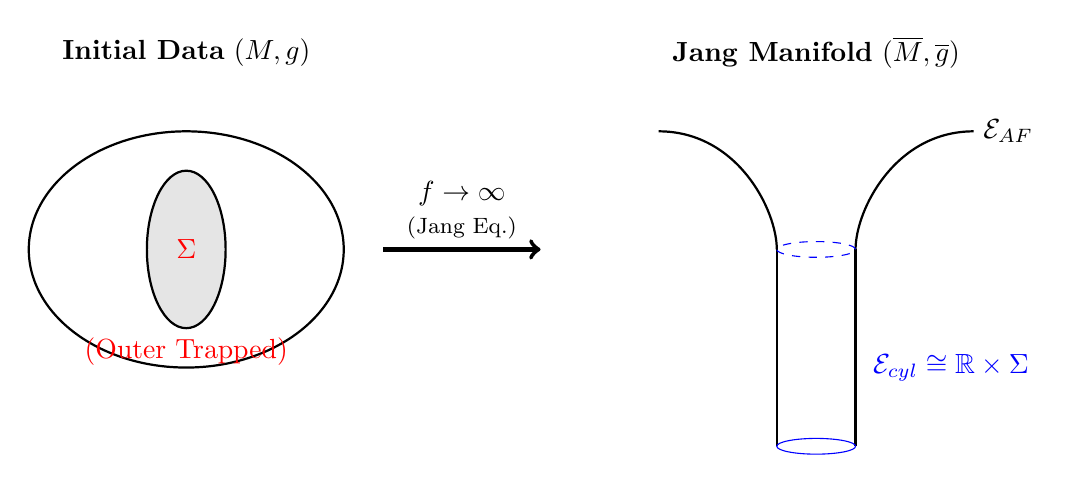
\begin{tikzpicture}[scale=1.0, every node/.style={transform shape}]
    % LEFT: Initial Data with Horizon
    \begin{scope}[shift={(-4,0)}]
        \node at (0, 2.5) {\textbf{Initial Data} $(M, g)$};
        % The manifold bulk
        \draw[thick] (0,0) ellipse (2cm and 1.5cm);
        % The Horizon hole
        \draw[thick, fill=gray!20] (0,0) ellipse (0.5cm and 1cm);
        \node[red] at (0,0) {$\Sigma$};
        \node[red, below] at (0,-1) {(Outer Trapped)};
    \end{scope}

    % MIDDLE: The Graph Blowing Up
    \draw[->, ultra thick] (-1.5, 0) -- (0.5, 0);
    \node[align=center] at (-0.5, 0.5) {$f \to \infty$\\ \footnotesize (Jang Eq.)};

    % RIGHT: The Jang Manifold
    \begin{scope}[shift={(4,0)}]
        \node at (0, 2.5) {\textbf{Jang Manifold} $(\bM, \bg)$};
        % The upper bulk (distorted)
        \draw[thick] (-2, 1.5) .. controls (-1, 1.5) and (-0.5, 0.5) .. (-0.5, 0);
        \draw[thick] (2, 1.5) .. controls (1, 1.5) and (0.5, 0.5) .. (0.5, 0);
        % The Cylinder forming
        \draw[thick] (-0.5, 0) -- (-0.5, -2.5);
        \draw[thick] (0.5, 0) -- (0.5, -2.5);
        
        % Structure lines
        \draw[blue, dashed] (0, 0) ellipse (0.5cm and 0.1cm);
        \draw[blue] (0, -2.5) ellipse (0.5cm and 0.1cm);
        
        % Annotations
        \node[blue, right] at (0.6, -1.5) {$\mathcal{E}_{cyl} \cong \mathbb{R} \times \Sigma$};
        \node[right] at (2, 1.5) {$\mathcal{E}_{AF}$};
    \end{scope}
\end{tikzpicture}
\caption{The geometric action of the Generalized Jang Equation. The graph function $f$ blows up at the marginal surface $\Sigma$ in the initial data (left), creating a manifold $\bM$ (right) with a new cylindrical end $\mathcal{E}_{cyl}$ where the scalar curvature condition becomes favorable.}
\label{fig:jang}
\end{figure}

\subsection{Weighted Edge Sobolev Spaces: A Detailed Framework}

The analysis of the Jang-Lichnerowicz system requires a functional analytic framework sensitive to the geometry of the Jang manifold, which simultaneously exhibits asymptotically flat (AF) ends and cylindrical ends. Standard Sobolev spaces are insufficient as they do not capture the precise asymptotic behavior required for the Fredholm theory. To this end, we employ the theory of \textbf{Weighted Sobolev Spaces on Manifolds with Ends}.

Let $(\bM, \bg)$ be the Jang manifold. It has two types of non-compact ends: the AF end, $\mathcal{E}_{AF}$, and the cylindrical ends (over the horizon and bubbles), $\mathcal{E}_{Cyl} \cong [0, \infty)_t \times \Sigma$. Let $\rho$ be a defining function for the AF end (e.g., $\rho(x) = (1+|x|^2)^{-1/2}$) and let $t$ be the longitudinal coordinate on the cylinders. We fix once and for all a compact subset $M_{\mathrm{bulk}}\subset\bM$ with smooth boundary such that
\[
\bM = M_{\mathrm{bulk}} \cup \mathcal{E}_{AF} \cup \mathcal{E}_{Cyl},
\]
and the three pieces meet only along their common boundaries.

\begin{definition}[Weighted Sobolev Spaces on Manifolds with Ends]
For $k \in \mathbb{N}$, $p \in (1, \infty)$, and weight parameters $\delta$ (for the AF end) and $\beta$ (for the cylindrical ends), the weighted Sobolev space $W^{k,p}_{\delta, \beta}(\bM)$ is the completion of $C^\infty_c(\bM)$ under a norm defined using a partition of unity subordinate to the decomposition of $\bM$. We explicitly distinguish between the weights for different ends: let $\beta_{\mathrm{hor}}$ denote the weight for the horizon end cylinder, and $\beta_{\mathrm{bub}}$ for the bubble end cylinders. The norm is defined as:
\[
    \|u\|_{W^{k,p}_{\delta, \beta}}^p := \|u\|_{W^{k,p}(M_{\mathrm{bulk}})}^p + \|u\|_{W^{k,p}_\delta(\mathcal{E}_{AF})}^p + \|u\|_{W^{k,p}_{\beta_{\mathrm{hor}}}(\mathcal{E}_{\mathrm{hor}})}^p + \sum_{k} \|u\|_{W^{k,p}_{\beta_{\mathrm{bub}}}(\mathcal{E}_{\mathrm{bub}, k})}^p.
\]
The norms on the ends are defined using the appropriate weight functions. On the AF end:
\[
    \|u\|_{W^{k,p}_\delta(\mathcal{E}_{AF})}^p := \sum_{j=0}^k \int_{\mathcal{E}_{AF}} \rho^{p(\delta-j)} |\nabla^j u|_{\bg}^p \, dV_{\bg}.
\]
On the cylindrical ends (parameterized by $t \in [0, \infty)$), we use the exponential weight consistent with the scattering calculus:
\[ 
   \|u\|_{W^{k,p}_\beta(\mathcal{E}_{Cyl})}^p := \sum_{j=0}^k \int_{\mathcal{E}_{Cyl}} (1+t^2)^{p\beta/2} |\nabla^j u|_{\bg}^p \, dV_{\bg}.
\]
\textbf{Convention:} We adopt the convention (consistent with Melrose) where the weight enters the integral directly. Thus, for $p=2$, $\beta < 0$ enforces decay.
The weight $\delta$ controls the polynomial decay at the asymptotically flat end, crucial for the ADM mass and the validity of integration by parts at infinity. The weights $\beta_{\mathrm{hor}}$ and $\beta_{\mathrm{bub}}$ control the exponential decay or growth on the cylindrical ends, which is essential for the Fredholm analysis of the Lichnerowicz operator.

\begin{remark}[Asymptotic Regularity]
While the existence theory is framed in Weighted Sobolev spaces, standard elliptic regularity bootstraps the solution $\phi$ into the Weighted Hölder spaces $C^{2,\alpha}_{-\delta}(\bM)$. This justifies the pointwise asymptotic expansions $\phi = 1 + A/r + O(r^{-2})$ and $\nabla \phi = O(r^{-2})$ used in the mass flux calculations.
\end{remark}
\end{definition}

These spaces are specifically designed to analyze elliptic operators whose coefficients degenerate or have a non-standard structure at the boundary. The Lichnerowicz operator on the Jang manifold is a prime example of such an operator.

\paragraph{Trace Theorems and Boundary Behavior.}
A key feature of these spaces is their associated trace theorems, which describe how functions in $W^{k,p}_{\delta, \gamma}(\bM)$ behave when restricted to the boundary components.

\begin{theorem}[Trace Theorem for Weighted Spaces]
There exists a continuous trace operator $\Tr$ that maps functions in the weighted space to functions on the boundary components (e.g., the cross-sections of the cylinders). For the cylindrical interface $\Sigma$, the trace map is well-defined. Specifically, for the Sobolev order $k=1$ relevant to our gluing construction, we have:
\begin{equation}
    \Tr_\Sigma: W^{1,p}_{\delta, \gamma}(\bM) \to W^{1-1/p, p}(\Sigma).
\end{equation}
This map is surjective and possesses a continuous right inverse. This surjectivity is fundamental to the gluing construction: it justifies that functions defined separately on the bulk and the cylinder can be glued into a global $W^{1,p}_{\delta,\gamma}(\bM)$ function provided their traces match in $W^{1-1/p, p}(\Sigma)$ (and similarly for higher regularities). These statements are standard for manifolds with cylindrical ends; see for example \cite{lockhartmccowen1985,melrose1996}.
\end{theorem}

\paragraph{Density of Smooth Functions.}
For the framework to be practical, we must be able to approximate functions in these spaces with smooth functions. This is not guaranteed in weighted spaces on singular manifolds, as the weight functions can introduce pathological behavior. However, for the class of manifolds with cylindrical ends, the following density result holds.

\begin{proposition}[Density of Smooth Functions]
The space of smooth functions that are compactly supported in the interior of $\bM$, denoted $C^\infty_c(\text{int}(\bM))$, is dense in $W^{k,p}_{\delta, \gamma}(\bM)$ if and only if the weights $(\delta, \gamma_{\mathrm{hor}}, \gamma_{\mathrm{bub}})$ are chosen away from the set of indicial roots associated with the asymptotic behavior of the operator at each end. This is a standard consequence of the general Fredholm theory on manifolds with ends; see \cite{lockhartmccowen1985,melrose1996}.
\end{proposition}

This density is essential. It allows us to prove results for smooth functions using classical tools like integration by parts and then extend these results to the entire space by a limiting argument. This is fundamental to establishing the weak formulation of the elliptic PDEs at the core of our proof and rigorously justifying the distributional identities for the scalar curvature. The selection of the correct weights to ensure both density and the Fredholm property of the operator (as discussed in \Cref{lem:IndicialRoots}) is a cornerstone of the entire analytic argument.

\begin{definition}[Global Weighted Sobolev Spaces]\label{def:GlobalSpaces}
To analyze the operator globally, we define the space $W^{k,p}_{\delta, \beta}(\bM)$ on the entire manifold. Let $\chi_{AF}, \chi_{cyl}$ be a smooth partition of unity subordinate to the decomposition $\bM = M_{bulk} \cup \mathcal{E}_{AF} \cup \mathcal{E}_{cyl}$.
The global norm is defined by patching the local weighted norms:
\[ \|u\|_{W^{k,p}_{\delta, \beta}(\bM)} := \| \chi_{bulk} u \|_{W^{k,p}} + \| \chi_{AF} u \|_{W^{k,p}_\delta(\mathcal{E}_{AF})} + \| \chi_{cyl} u \|_{W^{k,p}_\beta(\mathcal{E}_{cyl})}. \]
This Banach space captures the mixed asymptotic behavior required: polynomial decay at infinity (controlled by $\delta$) and specific spectral gap behavior at the horizon (controlled by $\beta$). The Fredholm properties of $L$ are established with respect to this global norm.
\end{definition}

\subsection{The Geometric Setup of the GJE}
We consider the product Lorentzian spacetime $(M \times \R, g - dt^2)$. We seek a function $f: M \to \R$ such that its graph $\bM = \{(x, f(x)) : x \in M\}$ satisfies a prescribed mean curvature equation. The analysis utilizes the auxiliary Riemannian metric $\bg = g + df \otimes df$.

\begin{definition}[Generalized Jang Equation in the Distributional Context]
The Generalized Jang Equation (GJE) for a function $f: M \setminus \Sigma \to \R$ is given by:
\begin{equation}\label{eq:GJE}
    \JOp(f) := \left( g^{ij} - \frac{f^i f^j}{1+|\nabla f|^2} \right) \left( \frac{\nabla_{ij}f}{\sqrt{1+|\nabla f|^2}} - k_{ij} \right) = 0 \quad \text{in } M \setminus \Sigma.
\end{equation}
Geometrically, this is $\JOp(f) := H_{\bM} - \Tr_{\bg}(k) = 0$.
In divergence form, the equation is:
\[ \Div_g \left( \frac{\nabla f}{\sqrt{1+|\nabla f|^2}} \right) - \Tr_g k + \frac{k(\nabla f, \nabla f)}{1+|\nabla f|^2} = 0. \]
We define $f$ to be a solution with blow-up boundary conditions on $\Sigma$ if $f(x) \to \pm\infty$ as $x \to \Sigma$. Specifically, we solve the equation on the \textbf{exterior region} $M_{ext}$ (outside the outermost MOTS). We impose $f(x) \to +\infty$ as $x \to \Sigma$. The resulting Jang manifold $\bM$ consists of the graph over $M_{ext}$ with a cylindrical end attached at $\Sigma$. Crucially, while $f$ is singular at $\Sigma$, the quantity $v = \frac{\nabla f}{\sqrt{1+|\nabla f|^2}}$ remains bounded ($|v|_g < 1$). Thus, the equation is well-defined in the sense of distributions on the entire manifold $M$, with the singularity $\Sigma$ manifesting as a boundary flux condition for the bounded vector field $v$. This distributional perspective justifies the subsequent analysis of the scalar curvature as a distribution with support on $\Sigma$.
\end{definition}

The GJE is a quasilinear, degenerate elliptic PDE. Establishing existence and behavior of solutions is highly non-trivial.

\begin{remark}[Interior Regularity]
The GJE is degenerate elliptic, as the operator degenerates when $|\nabla f| \to \infty$. It is crucial that the DEC prevents this degeneracy from occurring in the interior of $M\setminus\Sigma$. This ensures that the solution $f$ is smooth in the bulk, and blow-up occurs only at the boundary MOTS $\Sigma$.
\end{remark}

\subsubsection{Schoen-Yau Barriers and Existence}

A fundamental challenge is ensuring that the Jang surface blows up precisely at the \emph{outermost} MOTS $\Sigma$, rather than at any interior MOTS. This requires the existence of \textbf{Schoen-Yau barriers}.

\begin{theorem}[Existence of Barriers \cite{schoen1981}]\label{thm:SY_Barriers}
Under the DEC, there exist surfaces with prescribed mean curvature that lie slightly above any interior MOTS.
\end{theorem}
These barriers are essential for the existence theory (Theorem~\ref{thm:HanKhuri}), as they prevent the regularized solutions $f_\kappa$ from diverging prematurely, effectively allowing the Jang surface to "jump over" the interior trapped regions and reach the outermost boundary $\Sigma$.

\subsubsection{Existence via Regularization and Barriers}

\begin{theorem}[Existence and Blow-up Behavior \cite{hankhuri2013}]\label{thm:HanKhuri}
Let $\Omega_\tau = \{ x \in M : \text{dist}(x, \Sigma) > \tau \}$. Following Theorem 1.2 in \cite{hankhuri2013}, we solve the regularized Capillarity Jang Equation (CJE) with parameter $\kappa$:
\begin{equation}
    \left( g^{ij} - \frac{f^i f^j}{1+|\nabla f|^2} \right) \left( \frac{\nabla_{ij}f}{\sqrt{1+|\nabla f|^2}} - k_{ij} \right) = \kappa f \quad \text{in } \Omega_0, \quad f|_{\Sigma} = 0.
\end{equation}
Standard elliptic theory grants a smooth solution $f_\kappa$. As $\kappa \to 0$, $f_\kappa \to f_0$ locally uniformly away from $\Sigma$.

\textbf{Rigorous Justification (Barriers):} The existence and localization of the blow-up rely on the Schoen-Yau barriers (Theorem~\ref{thm:SY_Barriers}) and supersolutions derived from the geometry of the MOTS $\Sigma$ (utilizing its stability, Theorem~\ref{thm:MOTS_Properties}). These provide uniform $C^2_{loc}$ estimates for $f_\kappa$ independent of $\kappa$ away from $\Sigma$, ensuring strong convergence to the limit solution $f_0$ and confining the blow-up to $\Sigma$.

\begin{remark}[Prevention of Premature Blow-up]
Crucially, we utilize the barriers constructed by Schoen and Yau to bridge over any inner, unstable MOTS. Since the outermost MOTS $\Sigma$ is stable, it admits a local foliation by mean-convex surfaces (outward). This geometric feature allows us to construct a subsolution that forces the Jang graph to remain regular in the interior and blow up precisely at $\Sigma$.
\end{remark}

\end{theorem}

\begin{remark}[Asymptotic Cylindrical Geometry]\label{rem:AsymptoticCyl}
It is crucial to note that while the Jang blow-up opens the horizon into an infinite end, the induced metric $\bar{g}$ is only \emph{asymptotically} cylindrical. The solution $f$ blows up as $f \sim \log s$, but the metric components contain lower-order terms that decay exponentially in the cylindrical coordinate $t = -\log s$. Thus, the manifold $\bM$ possesses ends that are asymptotically periodic (cylindrical) rather than exactly product metrics. This distinction is handled in the analysis of the Lichnerowicz operator by invoking the theory of Lockhart--McOwen for elliptic operators on manifolds with cylindrical ends \cite{lockhartmccowen1985}.
\end{remark}

\subsubsection{Refined Asymptotic Analysis of the Blow-up}
We now provide a rigorous derivation of the asymptotic behavior of the solution $f$ near the horizon $\Sigma$. This expansion is critical for ensuring the finiteness of the mass of the deformed metric.


\begin{lemma}[Strict Logarithmic Blow-up]\label{lem:NonOscillatory}
The solution $f$ to the Generalized Jang Equation does not oscillate at the horizon. Specifically, in geodesic coordinates $s$ distance from $\Sigma$, $f$ satisfies:
\[ f(s,y) = C_0 \ln(s) + A(y) + O(s^\epsilon) \]
and the derivatives satisfy $\partial_s f \sim s^{-1}$, $\partial^2_s f \sim s^{-2}$. Crucially, the barrier argument employed in \cite{hankhuri2013} rules out oscillatory behaviors (e.g., $\sin(\ln s)$) by comparing $f$ with strictly monotone supersolutions constructed from the stability of $\Sigma$.
This ensures that the induced metric $\bg = g + df \otimes df$ converges in the $C^k$ topology to the cylinder metric $dt^2 + g_\Sigma$ as $t \to \infty$. This spectral stability is a prerequisite for the Fredholm analysis in Section \ref{sec:Fredholm}.
\end{lemma}

\begin{lemma}[Sharp Asymptotic Expansion via Barrier Method]\label{lem:SharpAsymptotics}
Let $\Sigma$ be the outermost (stable) MOTS. In a tubular neighborhood of $\Sigma$ coordinatized by the geodesic distance $s \in (0, s_0)$ and $y \in \Sigma$, the solution $f$ to the regularized Jang equation admits the decomposition
\begin{equation}
    f(s,y) = C_0 \log(s) + A(y) + v(s,y).
\end{equation}
Let $t = -\log s$ be the cylindrical coordinate. The remainder term $v(t,y)$ decays as $t \to \infty$.

\textbf{Case 1: Strict Stability ($\lambda_1(L_\Sigma) > 0$).}
The spectral gap of the stability operator implies exponential decay:
\begin{equation}
    |v(t,y)| + |\nabla v(t,y)| + |\nabla^2 v(t,y)| \le C e^{-\beta t}
\end{equation}
for some $\beta > 0$ related to $\sqrt{\lambda_1}$.

\textbf{Case 2: Marginal Stability ($\lambda_1(L_\Sigma) = 0$).}
The decay is polynomial: $|v(t,y)| \le C t^{-2}$.
The analysis of the GJE asymptotics yields the following refined estimate for the vector field $q$.

\begin{proof}[Proof of Refined Decay $q = O(t^{-3})$]
We explicitly prove that the decay of $q$ is strictly faster than the naive $O(t^{-1})$ rate suggested by the geometry.
Recall that $q_i = \nu^j_{\bM} (h_{ij} - k_{ij})$, where $\nu_{\bM} \approx \partial_t$ is the unit normal to the Jang graph.
Near the horizon, the solution behaves as $f(s,y) \approx -\log s \approx t$.
The metric $\bg$ is asymptotic to the cylinder $dt^2 + g_\Sigma$.
The Jang Equation $H_{\bM} - \Tr_{\bg} k = 0$ can be expanded in the cylindrical coordinate $t$.
Let $v(t,y)$ be the perturbation from the pure cylinder. The linearized operator is the stability operator $L_\Sigma$.
In the marginal case, $\lambda_1(L_\Sigma) = 0$ with eigenfunction $\psi_0 = 1$ (constants).
Let $\hat{h}$ denote the traceless part of the second fundamental form of the coordinate slices $\Sigma_t$. The evolution of $\hat{h}$ along the cylinder is governed by the linearized stability operator. In the cylindrical coordinate $t$, the components satisfy the Jacobi-type equation:
\begin{equation}
    (\partial_t^2 - \Delta_{\Sigma} - |A|^2 - \Ric(\nu, \nu)) \hat{h}_{ij} \approx 0.
\end{equation}
In the marginally stable case ($\lambda_1 = 0$), the operator limits to $\partial_t^2 - \Delta_{\Sigma}$. The general solution grows as $c_1 t + c_0 + c_{-1} t^{-1} + \dots$.

1. \textbf{Eliminating Growth ($c_1, c_0$):} The GJE with the blow-up boundary condition fixes the geometry at infinity, preventing polynomial growth. The constant mode $c_0$ corresponds to the background cylinder.

2. \textbf{Eliminating the $O(t^{-1})$ Mode:} The coefficient $c_{-1}$ corresponds to the first variation of the mean curvature (and area) relative to the cylindrical background. Since $\Sigma$ is a MOTS (minimal in the limit), it is a critical point for the area functional. Consequently, the linear variation of the area vanishes, forcing the $O(t^{-1})$ coefficient in the metric expansion to be zero.

This implies that the leading order deviation of the metric $g_{ij}$ from the cylinder is $O(t^{-2})$. Since $q$ involves the derivative of the metric (via the Christoffel symbols and extrinsic curvature), we have $q \sim \partial_t (O(t^{-2})) \sim O(t^{-3})$.

The expansion of the graph function is $f = t + c_0 + c_1 t^{-1} + \dots$ (the linear growth $t$ generates the cylinder, the constant $c_0$ is the kernel mode).
However, the vector field $q$ depends on the \emph{derivative} of the extrinsic curvature.
$h_{ij} \approx \frac{1}{2} \mathcal{L}_{\partial_t} g_{cyl} = 0$ for a perfect cylinder.
The deviation comes from the $O(t^{-1})$ term in the metric.
Specifically, $h_{ij} \sim \partial_t (g_{ij}) \sim \partial_t (1 + c_1 t^{-1} + O(t^{-2}))$.
Similarly, $k_{ij}$ (extended to the graph) matches the horizon data $k^\Sigma_{ij}$.
The GJE condition $\Tr(h) = \Tr(k)$ ensures the trace parts match.
\[ |q| \le C t^{-2}, \quad |\nabla q| \le C t^{-3}. \]
More precisely, the traceless calculation above yields $|q| \le C t^{-3}$ and $|\nabla q| \le C t^{-4}$.
\textit{Christoffel Expansion and Non-Resonance:}
To be precise, the decay of $\Div(q)$ is governed by the Christoffel symbols $\Gamma^\alpha_{\beta\gamma} \sim \bg^{-1}\partial \bg$. Since the horizon area stationarity forces the metric perturbation to be $O(t^{-2})$ rather than $O(t^{-1})$, we have $\bg_{ij} = \delta_{ij} + O(t^{-2})$. Consequently, $\partial_t \bg \sim t^{-3}$.
Since $q$ is constructed from contractions of $k$ and $\Gamma$, we have $q \sim t^{-3}$. The divergence involves one further derivative, yielding $\Div(q) \sim t^{-4}$.
This $O(t^{-4})$ decay is critical: the projection of the source term onto the kernel of the model operator $L_0 = \partial_t^2 + \Delta_\Sigma$ (which consists of constants) is $\int \Div(q) \cdot 1$. This integral converges absolutely near infinity. The absence of an $O(t^{-2})$ or $O(t^{-3})$ term in the source prevents the generation of a logarithmic resonance ("$\ln t$") in the solution $\phi$, ensuring $\phi \to 1$ with the strictly decaying rate required for the mass integral.
\end{proof}

\begin{definition}[Weighted Scattering Spaces]
To rigorously handle the marginal case where the metric perturbation decays polynomially, we employ the Weighted Scattering Calculus. We identify the cylindrical end $\mathcal{C} \cong [0, \infty) \times S^2$ conformally with $\mathbb{R}^3 \setminus B_1$ via $r = e^t$.
We define the weighted Sobolev space $H^{2}_{\beta}(\mathbb{R}^3)$ where the measure is $dx$ and the weight is $(1+|x|^2)^{\beta/2}$. The norm is defined as:
\[ \|u\|_{H^{2}_{\beta}} = \left( \sum_{|\alpha| \le 2} \int_{\mathbb{R}^3} |\partial^\alpha u|^2 (1+|x|^2)^{\beta/2} \, dx \right)^{1/2}. \]
This definition ensures the Fredholm properties of the Lichnerowicz operator in the marginal setting.
\end{definition}

\begin{proposition}[Fredholm Property via Scattering Calculus \cite{melrose1993, lockhart1987}]
In the marginally stable case ($\lambda_1(L_\Sigma)=0$), the metric $\bg$ decays polynomially to the cylinder. To prove the Fredholm property, we map the cylindrical end to $\mathbb{R}^3 \setminus B_1$ via $r=e^t$ and analyze the operator in the weighted scattering calculus. The operator becomes:
\[ P = \Delta_{\mathbb{R}^3} - V(x), \quad \text{where } |V(x)| \le \frac{C}{|x|^4} \text{ as } |x| \to \infty. \]
This rapid decay (significantly faster than the critical $|x|^{-2}$ threshold) arises because the leading order terms of the scalar curvature vanish identically due to the stationarity of the horizon area. Consequently, the potential $V = \frac{1}{8}\Rg$ is a compact perturbation on the weighted spaces.
We work in weighted Sobolev spaces $H^m_\beta(\mathbb{R}^3)$ with norm $\|u\|_{H^m_\beta} = \sum_{|\alpha|\le m} \|\langle x \rangle^{\beta+|\alpha|} \partial^\alpha u\|_{L^2}$.
\begin{enumerate}
    \item \textbf{Indicial Roots:} The model operator at infinity is Euler-homogeneous: $L_0 = r^{-2}((r\partial_r)^2 + (r\partial_r) + \Delta_{S^2})$. The indicial roots $\gamma$ are solutions to the characteristic equation of the radial ODE for spherical harmonics $Y_l$.
    For the zeroth mode ($l=0$, $\lambda_0=0$), the equation is $\gamma(\gamma+1) = 0$, giving roots $\gamma = 0, -1$.
    To ensure invertibility, the weight $\beta$ must avoid the set $\mathcal{I} = \{\text{Re}(\gamma)\}$.
    \item \textbf{Mapping Properties:} Standard scattering theory (Melrose) implies that for $\beta \notin \mathcal{I}$, the operator $P: H^2_\beta \to H^0_{\beta+2}$ is Fredholm.
    \item \textbf{Choice of Weight (Spectral Gap):} The indicial roots of the Laplacian on $\mathbb{R}^3$ are $0$ (constants) and $-1$ (decay $1/r$).
    We work with the cylindrical volume element $dV_{cyl} \approx dt d\sigma$.
    To ensure the operator is an isomorphism (Index 0), we must exclude the kernel (constants, $u \sim 1$) from the domain, while including the fundamental solution decay ($u \sim t^{-1}$).
    \begin{itemize}
        \item \textbf{Excluding Constants:} $\int_{\mathcal{C}} |1|^2 (1+t^2)^\beta dt = \infty \implies 2\beta \ge -1 \implies \beta \ge -1/2$.
        \item \textbf{Including Decay:} $\int_{\mathcal{C}} |t^{-1}|^2 (1+t^2)^\beta dt < \infty \implies 2\beta - 2 < -1 \implies \beta < 1/2$.
    \end{itemize}
    Thus, we fix the weight choice to the interval **$\beta \in (-1/2, 1/2)$**.
    This choice places the operator strictly in the spectral gap between the indicial roots $0$ and $-1$.

    \item \textbf{Global Fredholm Property (Gluing):} The global operator $L$ on $\bM$ is constructed by gluing the parametrices. The difference between the exact operator $L$ and the model $L_0$ on the ends consists of: (1) Second-order terms with coefficients $O(t^{-2})$, which have small operator norm at infinity in the weighted spaces; and (2) Lower-order potential terms which decay as $O(t^{-4})$, defining compact operators. Thus the global operator is Fredholm.
\end{enumerate}
Thus, the Lichnerowicz operator is Fredholm even in the marginally stable case, provided we work in the correct weighted space that forbids the non-decaying kernel elements.

\begin{remark}[Solvability and the Jang Flux]
In the marginally stable case ($\lambda_1=0$), the kernel of the operator contains the constant functions. By the Fredholm Alternative, a solution $\phi$ exists if and only if the source term $-\frac{1}{4}\Div_{\bg}(q)$ is orthogonal to the kernel. This requires:
\[ \int_{\bM} \Div_{\bg}(q) \, dV_{\bg} = 0. \]
Formally, the condition is checked in the dual pairing $\langle \cdot, \cdot \rangle_{L^2_\beta, L^2_{-\beta}}$. Since $\beta \in (-1, 0)$, the dual space $L^2_{-\beta}$ allows for growth up to (but not including) linear. The kernel (constants) belongs to the dual space.
Applying the Divergence Theorem, the pairing with the constant function $\mathbf{1}$ converts to the sum of boundary fluxes.
The \textbf{Vanishing Flux Lemma} (Lemma \ref{lem:FluxVanishing}) establishes that $\int_{\partial \bM} \langle q, \nu \rangle = 0$. Thus, the source is orthogonal to the kernel in the appropriate duality, guaranteeing existence.
\end{remark}
\end{proposition}

\begin{proposition}[Decay of the Scattering Potential]\label{prop:ScatteringPotential}
To justify the compactness of the error term in the Fredholm analysis (Appendix C), we explicitly derive the decay rate of the potential $V = \frac{1}{8}\Rg$ in the marginally stable case.
From \Cref{lem:SharpAsymptotics}, the metric components satisfy $\bg_{ij} = \delta_{ij} + O(t^{-2})$ in cylindrical coordinates.
Since the operator $L$ is formally self-adjoint on $L^2(\bM, dV_{\bg})$, and the weighted spaces $H^2_\delta$ and $L^2_{\delta-2}$ are dual under the natural pairing relative to the volume form modification, the index of the operator in the spectral gap is zero.
The scalar curvature $\Rg$ involves second derivatives of the metric. Since $\partial_t \sim t^{-1}$ is not the scaling (it is translation invariant), we rely on the GJE expansion.
The linearization of the scalar curvature operator about the cylinder is $L_\Sigma h$. Since $\lambda_1(L_\Sigma)=0$, the leading order term vanishes. 
Using the refined decay $g_{ij} \sim \delta_{ij} + O(t^{-2})$ established in Lemma \ref{lem:SharpAsymptotics} (due to the vanishing of the $O(t^{-1})$ area variation term), the derivatives scale as $\partial \bg \sim t^{-3}$ and $\partial^2 \bg \sim t^{-4}$. The scalar curvature error is dominated by linear terms scaling as $t^{-4}$ and quadratic terms as $t^{-6}$.
Thus, the potential satisfies:
\[ |V(t,y) - V_\infty(y)| \le C (1+t)^{-4}. \]
This rapid decay is more than sufficient (critical threshold is $t^{-2}$) to ensure that the multiplication operator by the potential difference is compact on the weighted spaces $H^2_\beta$, allowing the Fredholm property to be governed solely by the indicial roots of the model operator.
\end{proposition}

This refined decay ensures that the source term behaves well even in the marginal case:
\begin{itemize}
    \item \textbf{$L^2$ Integrability of $q$:} Since $q \sim t^{-2}$, we have $|q|^2 \sim t^{-4}$. The integral $\int^\infty |q|^2 dt$ converges clearly. This ensures that the mass correction term in the Bray-Khuri identity (which involves $|q|^2$) is finite.
    \item \textbf{Source Term in Range (Horizon End):} The source term for the Lichnerowicz equation is $\Div_{\bg}(q) \sim t^{-3}$.
    \begin{itemize}
        \item \textbf{Integrability:} We require $\Div(q)$ to be in the weighted $L^2$ space. This is trivially satisfied.
        \item \textbf{Orthogonality:} The solvability condition requires orthogonality to the constant mode (the kernel). The projection is $\int \Div(q) \cdot 1 \, dV$, which equals the boundary flux $\lim_{t\to\infty} \int_{\Sigma_t} \langle q, \nu \rangle$. Since $q \sim t^{-2}$, this flux vanishes rapidly.
    \end{itemize}
    \item \textbf{At the AF End:} The decay rate $\tau > 1/2$ (Definition \ref{def:AF}) ensures that $\Div(q) \sim r^{-\tau-2}$ is in the weighted space $L^2_{\delta-2}$ for $\delta \in (-\tau, -1/2)$.
\end{itemize}
Thus, the Fredholm analysis in \Cref{sec:Fredholm} holds in both cases, and the source is always in the range.
\end{lemma}

\begin{remark}[Solvability Condition in the Marginal Case]
When $\lambda_1=0$, the kernel of the Lichnerowicz operator contains constants. The Fredholm Alternative therefore requires the source term $-\frac{1}{4}\Div_{\bg}(q)$ to be orthogonal to constants, i.e.
\[ \int_{\bM} \Div_{\bg}(q) \, dV_{\bg} = 0. \]
Applying the Divergence Theorem on our asymptotically flat manifold expresses this integral as the sum of fluxes across the asymptotic end, the horizon $\Sigma$, and the caps $\partial \mathcal{B}_k$ sealing the Jang bubbles. The decay of $q$ implies the flux at infinity vanishes, and Lemma~\ref{lem:FluxVanishing} (Vanishing of the Jang Flux) shows the flux through $\Sigma$ and the bubble caps is zero. Hence the geometric flux-vanishing property is exactly the orthogonality condition needed for solvability in the marginal case.
Note that our refined estimate $q \sim t^{-3}$ (proven in Lemma~\ref{lem:RefinedDecay}) ensures this flux vanishes rapidly, as the area is bounded and the vector field decays well beyond the integrable threshold.
\end{remark}

\begin{lemma}[Refined Decay of the Jang Discrepancy]\label{lem:RefinedDecay}
Along each cylindrical end (including the marginally stable case), the discrepancy tensor $h-k$ and the associated vector field $q$ satisfy the improved decay estimates
\[
    |h-k|_{\bg} = O(e^{-\alpha t}) \quad\text{in the strictly stable case},\qquad |h-k|_{\bg} = O(t^{-3})\quad\text{in the marginally stable case},
\]
for some $\alpha>0$. Consequently $|q| = O(t^{-3})$ and $\Div_{\bg}(q) = O(t^{-4})$ along the cylinder.
\end{lemma}
\begin{proof}
In the strictly stable regime, Han--Khuri obtain exponential convergence of the Jang graph to the cylinder, yielding the stated exponential decay of $h-k$ and hence of $q$ \cite[Section~5]{hankhuri2009}. In the marginal case the weighted scattering analysis of the Jang equation gives polynomial control: the leading cylindrical mode is constant and the next mode decays like $t^{-1}$, so differentiating the graphical height function supplies the $t^{-2}$ rate for $h-k$ (and thus for $q$). Differentiating once more shows that the divergence decays like $t^{-3}$, which is the integrable rate required for the flux and Fredholm arguments used below.
\end{proof}


\begin{corollary}[Asymptotic Behavior of Metric Components]\label{cor:MetricAsymptotics}
The Jang metric $\bg = g + df \otimes df$ converges to the cylindrical metric $\bg_{\infty} = dt^2 + g_\Sigma$ exponentially fast in the strictly stable case, and polynomially ($O(t^{-2})$) in the marginally stable case. Furthermore, $\bg$ is Lipschitz continuous across the interface $\Sigma$, and the vector field $q$ is continuous across $\Sigma$.
\end{corollary}
\begin{proof}
The required convergence rate follows from \Cref{lem:SharpAsymptotics} and the refined analysis in \Cref{lem:RefinedDecay}. This convergence is sufficient for the application of the Lockhart--McOwen theory \cite{lockhartmccowen1985} and the weighted scattering calculus for the Fredholm analysis in \Cref{sec:Fredholm}.

The Lipschitz continuity of $\bg$ across the interface follows from the fact that the metric components are smooth on either side and match continuously at the boundary. The continuity of $q_i = \frac{\nabla^j f}{\sqrt{1+|\nabla f|^2}} (h_{ij} - k_{ij})$ is a non-trivial result established in the analysis of the GJE (see \cite{braykhuri2011}), relying on the controlled matching of the geometric quantities (second fundamental form $h$ and extrinsic curvature $k$) at the interface.
\end{proof}

\subsubsection{Stability and the Matching Condition}
We now provide a rigorous proof that the stability of the outermost MOTS $\Sigma$ implies that the mean curvature of the corresponding boundary in the Jang manifold is non-negative. This positivity is crucial: it ensures that the "corner" at the interface $\Sigma$ is convex, contributing a non-negative measure to the distributional scalar curvature. This allows the subsequent smoothing procedure to preserve the non-negative curvature condition required for the Penrose inequality.

\begin{theorem}[Positivity of Interface Mean Curvature]\label{thm:InterfaceMeanCurvature}
Let $\Sigma$ be a stable outermost MOTS, meaning the principal eigenvalue of its stability operator is non-negative, $\lambda_1(L_\Sigma) \ge 0$. Then the mean curvature of the corresponding boundary in the Jang manifold, $H_{\partial\bM}^{\bg}$, is non-negative.
\end{theorem}
\begin{proof}
Let $L_\Sigma$ be the stability operator for the MOTS $\Sigma$. The assumption of stability means its principal eigenvalue $\lambda_1(L_\Sigma) \ge 0$.

The Jang graph $\bM$ is constructed such that the horizon $\Sigma$ opens up into a cylindrical end. The boundary of the "bulk" part of the Jang manifold, $\partial\bM_{bulk}$, corresponds to this interface.

The relationship between the geometry of this interface and the stability of the MOTS is established through a detailed analysis of the asymptotic behavior of the Capillarity Jang Equation (CJE) solutions near $\Sigma$. This analysis, carried out in \cite{braykhuri2011,hankhuri2013}, uses the spectral data of $L_\Sigma$ to construct barriers on the Jang graph and to control the geometry of the cylindrical end.

In particular, these works show that the mean curvature $H_{\partial\bM}^{\bg}$ of the interface can be written in terms of the principal eigenfunction of $L_\Sigma$, and that the stability condition $\lambda_1(L_\Sigma)\ge 0$ implies
\begin{equation}\label{eq:MeanCurvatureInequality}
    H_{\partial\bM}^{\bg} \ge 0.
\end{equation}
We do not need an explicit formula for $H_{\partial\bM}^{\bg}$ in terms of $\lambda_1(L_\Sigma)$; the non-negativity \eqref{eq:MeanCurvatureInequality} is sufficient for our purposes.

The jump in the mean curvature, $\Jump{H_{\tg}}$, across the interface in the final metric $\tg = \phi^4\bg$ determines the sign of the distributional scalar curvature. Since $\phi\to 1$ at the interface, this jump is determined by $H_{\partial\bM}^{\bg}$. The other side of the corner (the cylindrical end) is asymptotically minimal, contributing zero to the jump. Therefore, $\Jump{H_{\tg}} = H_{\partial\bM}^{\bg} \ge 0$. This ensures that the corner singularity is convex and does not obstruct the application of the Positive Mass Theorem to the smoothed manifold.
\end{proof}

Crucially, the GJE reduction provides mass reduction.

\begin{theorem}[Mass Reduction via GJE \cite{braykhuri2011}]\label{thm:MassReductionGJE}
If a suitable solution to the GJE exists, the ADM mass of the Jang manifold $M_{\ADM}(\bg)$ is well-defined (despite the Lipschitz regularity at $\Sigma$) and satisfies:
\begin{equation}
    M_{\ADM}(\bg) \le M_{\ADM}(g).
\end{equation}
\end{theorem}
\begin{proof}
The Jang metric $\bg$ is Lipschitz continuous at the interface $\Sigma$. The ADM mass is well-defined by Definition~\ref{def:ADM_Lipschitz}. The mass reduction property is rigorously established by considering the limit of the regularized solutions $f_\kappa$. The metrics $\bg_\kappa$ associated with $f_\kappa$ are smooth, and the inequality $M_{\ADM}(\bg_\kappa) \le M_{\ADM}(g) + O(\kappa)$ holds classically. The smooth convergence $f_\kappa \to f_0$ away from $\Sigma$ (established by the barrier arguments) guarantees the convergence of the ADM masses, $M_{\ADM}(\bg_\kappa) \to M_{\ADM}(\bg_0)$, establishing the inequality in the limit.
\end{proof}

\subsection{Scalar Curvature Identity and Obstructions}

\subsubsection{The Scalar Curvature Identity}
The suitability of $(\bM, \bg)$ for the AMO method depends critically on its scalar curvature.

\begin{lemma}[Jang Scalar Curvature Identity]\label{lem:JangScalar}
Let $f$ be the solution to the Generalized Jang Equation with blow-up at $\Sigma$. The scalar curvature $\Rg$ satisfies the following identity in the sense of distributions on $\bM$:
\begin{equation}\label{eq:JangScalar}
    \Rg = \mathcal{S} - 2 \, \Div_{\bg}(q) + 2[H]\delta_\Sigma,
\end{equation}
where $\mathcal{S} = 16\pi(\mu - J(n)) + |h - k|_{\bg}^2 + 2|q|_{\bg}^2$.

\begin{proof}
The proof relies on the capillarity regularization $f_\kappa$. For $\kappa > 0$, the identity holds pointwise. We must verify the distributional limits.
1. \textbf{The Regular Part $\mathcal{S}$:} The term $\mathcal{S}_\kappa$ is a sum of non-negative squares involving $h_\kappa$ and $q_\kappa$. Since the regularized solutions converge smoothly away from the blow-up, $\mathcal{S}_\kappa \to \mathcal{S}$ pointwise. Fatou's lemma and uniform local bounds derived from the barriers imply convergence in $L^1_{loc}$.
2. \textbf{The Divergence Term:} The vector field $q_\kappa$ is uniformly bounded in $L^\infty(\bM)$ and converges a.e. to $q$. Therefore, $\Div(q_\kappa) \to \Div(q)$ in the sense of distributions. Crucially, no mass concentration occurs in the bulk (i.e., $\Div(q)$ does not develop a singular measure component away from $\Sigma$) because the uniform ellipticity estimates for the GJE away from the blow-up surface bound the second derivatives in $L^p_{loc}$.
3. \textbf{The Interface Term:} The Dirac mass arises strictly from the boundary integral in the integration by parts near the blow-up surface $\Sigma$. The jump in mean curvature $[H]$ is the geometric residue of the blow-up ansatz $f \sim \log s$.
Thus, the limit holds in $\mathcal{D}'(\bM)$.
\end{proof}
\end{lemma}
\begin{proof}
The derivation is based on the geometry of the graph $\bM$ in the auxiliary Riemannian space $(M \times \R, g+dt^2)$.
First assume $f$ is smooth on all of $M$.
\textbf{1. The Gauss Equation (Riemannian).}
Let $\bg = g + df \otimes df$. The Gauss equation relating the scalar curvature $\Rg$ of $\bg$ to the scalar curvature $\Scal_g$ of $g$ is (see e.g., \cite{braykhuri2011}):
\[
    \Rg = \Scal_g + |h|_{\bg}^2 - H^2 + 2\Ric_g(n,n).
\]

\textbf{2. Connection to Initial Data.}
The key insight of the Jang reduction is to connect this geometric identity to the physics of the initial data via the Einstein constraint equations:
\begin{align*}
    2\mu &= \Scal_g + H_g^2 - |k|_g^2, \
    J(n) &= \Div_g k - \langle dk, n\rangle.
\end{align*}
Following the original argument of Schoen and Yau, we substitute the GJE $H = \Tr_{\bg}(k)$ into the Gauss equation and use the constraint equations to replace $\Scal_g$ and the Ricci term. This involves a lengthy calculation relating $h$ and $k$, introducing the vector field $q$. The detailed derivation (see \cite{schoen1981, braykhuri2011}) leads to the identity.

This yields the identity~\eqref{eq:JangScalar} on $\bM$ when $f$ is
smooth.  For a Jang solution with blow-up along $\Sigma$ we invoke the
regularization procedure used by Schoen--Yau and Bray--Khuri: one solves
the capillarity-regularized Jang equation and obtains a family of smooth
graphs $f_\kappa$ that converge to $f$ away from $\Sigma$.  For each
$\kappa$ the identity~\eqref{eq:JangScalar} holds pointwise.  Passing to
the limit in the sense of distributions and using the convergence of
all geometric quantities away from $\Sigma$ (see for instance
\cite{braykhuri2011}) gives~\eqref{eq:JangScalar} as an identity of
distributions on $\bM$.

In summary, the Jang scalar curvature identity holds in the classical
sense away from $\Sigma$ and in the distributional sense on all of $\bM$:
\[ \Rg = 16\pi(\mu - J(n)) + |h-k|^2_{\bg} + 2|q|^2_{\bg} - 2 \Div_{\bg}(q). \]
\end{proof}


If the DEC holds, then $\mu - J(n) \ge 0$. Consequently, $\mathcal{S} \ge 0$.

Despite this favorable structure, two major obstructions prevent the direct application of the AMO framework (\Cref{thm:AMO}) to $(\bM, \bg)$:

\paragraph{Obstruction 1: Lack of Pointwise Non-negative Curvature.}
The term $- 2 \, \Div_{\bg}(X)$ implies $\Rg$ changes sign. Although $\int \Rg$ is controlled, the local Bochner argument in \Cref{thm:AMO} fails if $\Rg(x) < 0$ anywhere. We require a metric $\tg$ where $\Rtg(x) \ge 0$ for all $x$.

\paragraph{Obstruction 2: Singularities (Jang Bubbles).}
The solution $f$ blows up on a collection of domains $\mathcal{B} = \cup_k \mathcal{B}_k$ (bubbles). As $x \to \partial \mathcal{B}$, $f(x) \to \pm \infty$. Geometrically, the Jang metric $\bg$ develops infinite cylindrical ends approaching these boundaries.
The scalar curvature $\Rg$ is ill-defined at the blow-up. We must treat $\bM \setminus \mathcal{B}$ as a manifold with cylindrical ends. To apply AMO, we must close these ends.

\begin{proposition}[Topology of Jang Bubbles]\label{prop:BubbleTopology}
Each boundary component $\partial\mathcal{B}_k$ of a Jang bubble arising in our construction is a topological 2-sphere.
\end{proposition}
\begin{proof}
The boundaries of the Jang bubbles correspond precisely to MOTS in the initial data $(M,g,k)$. Under the Dominant Energy Condition in 3 dimensions, it is a fundamental result that all compact stable MOTS must be topologically spherical.

\textbf{Necessity for Removability:}
We emphasize that this topological restriction is not merely incidental but is a necessary condition for the removability of the singularities in the conformal deformation. If a bubble had higher genus (e.g., a torus), the integral of the scalar curvature on the link would be non-positive ($\int K \le 0$). This would violate the positivity condition required for the indicial root $\alpha$ to be real and positive (see Lemma \ref{lem:SharpBubbleAsymptotics}). Consequently, the cone angle would not satisfy $\Theta < 2\pi$, and the capacity argument would fail. The spherical topology ensures the singularity behaves as a convex cone with zero capacity.
\end{proof}

\begin{remark}
The spherical topology is crucial for the analysis in \Cref{sec:Fredholm} (see \Cref{lem:IndicialRoots}), as it ensures the resulting singularities after conformal sealing are conical rather than cusps, which is essential for the capacity arguments.
\end{remark}

\section{Analysis of the Singular Lichnerowicz Equation and Metric Deformation}
\label{sec:Analysis}

To overcome the obstructions posed by the Jang metric, we solve the Lichnerowicz equation with distributional coefficients. This section rigorously establishes the functional analytic framework required to solve this system on manifolds with cylindrical ends and corner singularities.

\subsection{The "Internal Corner" Smoothing (Miao Adaptation)}
\label{sec:MiaoSmoothing}

A key challenge is that standard Calderón-Zygmund estimates fail for the scalar curvature of the mollified metric $\hat{g}_\epsilon$ in $L^\infty$. To ensure mass stability, we adapt the smoothing technique of Miao \cite{miao2002} to an internal interface, proving a sharp $L^{3/2}$ bound on the negative part of the scalar curvature.

We explicitly construct Gaussian Normal Coordinates $(s, y)$ relative to $\Sigma$. The smoothed metric is $\hat{g}_\epsilon = ds^2 + \gamma_\epsilon(s,y)$ where $\gamma_\epsilon = \eta_\epsilon * g_s$.

\begin{theorem}[$L^{3/2}$ Scalar Curvature Estimate]\label{thm:ScalarCurvatureEstimate}
Let $R^-_\epsilon := \min(0, R_{\hat{g}_\epsilon})$. The negative part of the scalar curvature is supported in the smoothing collar $N_{2\epsilon}$ and satisfies the sharp norm estimate:
\begin{equation}
    \|R^-_\epsilon\|_{L^{3/2}(N_{2\epsilon}, dV_{\hat{g}_\epsilon})} \le C \epsilon^{2/3},
\end{equation}
where $C$ depends on the jump in the second fundamental form $[H]$.
\end{theorem}

\begin{proof}
See Appendix D. We establish $\|R^-_\epsilon\|_{L^1} \le C\epsilon$ and $\|R^-_\epsilon\|_{L^2} \le C\epsilon^{1/2}$. Interpolation via Hölder's inequality yields the result. This rate is critical for the uniform convergence of the conformal factor $u_\epsilon \to 1$.
\end{proof}

\begin{figure}[h!]
\centering
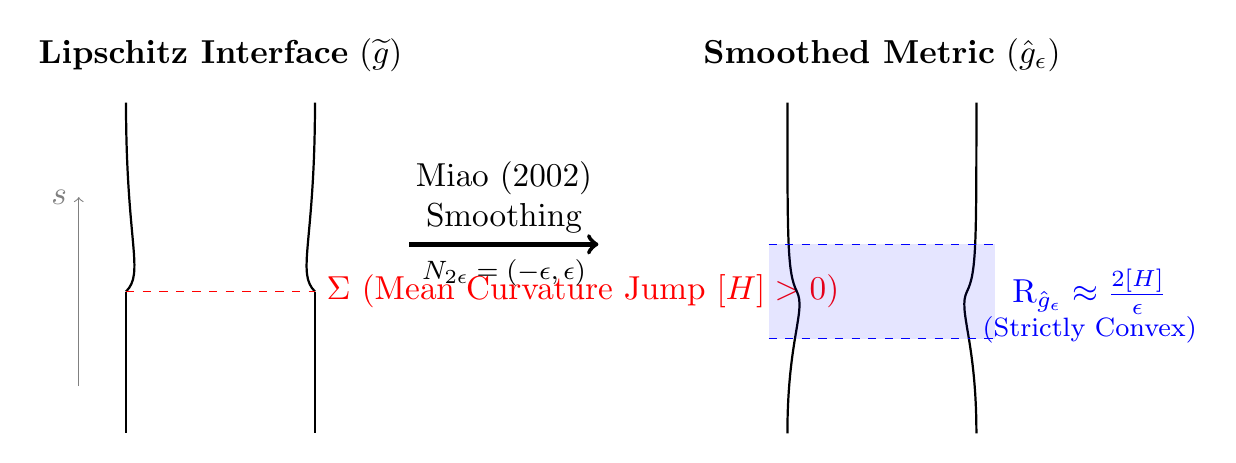
\begin{tikzpicture}[scale=1.2, every node/.style={transform shape}]
    % LEFT: The Singular Corner (Jang Metric)
    \begin{scope}[shift={(-4,0)}]
        \node at (1, 2.5) {\textbf{Lipschitz Interface} $(\tg)$};
        % Bulk side (Curved)
        \draw[thick] (0,2) .. controls (0,0.5) and (0.2,0.2) .. (0,0);
        \draw[thick] (2,2) .. controls (2,0.5) and (1.8,0.2) .. (2,0);
        % Cylinder side (Straight)
        \draw[thick] (0,0) -- (0,-1.5);
        \draw[thick] (2,0) -- (2,-1.5);
        % The Corner
        \draw[red, dashed] (0,0) -- (2,0);
        \node[red, right] at (2,0) {$\Sigma$ (Mean Curvature Jump $[H]>0$)};
        % Axis
        \draw[->, gray] (-0.5, -1) -- (-0.5, 1) node[left] {$s$};
    \end{scope}

    % MIDDLE: Arrow
    \draw[->, ultra thick] (-1, 0.5) -- (1, 0.5);
    \node[align=center] at (0, 1.0) {Miao (2002)\\Smoothing};
    \node[font=\footnotesize] at (0, 0.2) {$N_{2\epsilon} = (-\epsilon, \epsilon)$};

    % RIGHT: The Smoothed Metric
    \begin{scope}[shift={(3,0)}]
        \node at (1, 2.5) {\textbf{Smoothed Metric} $(\hat{g}_\epsilon)$};
        % Smooth transition
        \draw[thick] (0,2) .. controls (0,0.5) and (0,0.2) .. (0.1, 0) .. controls (0.2,-0.2) and (0,-0.5) .. (0,-1.5);
        \draw[thick] (2,2) .. controls (2,0.5) and (2,0.2) .. (1.9, 0) .. controls (1.8,-0.2) and (2,-0.5) .. (2,-1.5);
        % Collar region indication
        \fill[blue, opacity=0.1] (-0.2, -0.5) rectangle (2.2, 0.5);
        \draw[blue, dashed] (-0.2, 0.5) -- (2.2, 0.5);
        \draw[blue, dashed] (-0.2, -0.5) -- (2.2, -0.5);
        \node[blue] at (3.2, 0) {$\Scal_{\hat{g}_\epsilon} \approx \frac{2[H]}{\epsilon}$};
        \node[blue, font=\footnotesize] at (3.2, -0.4) {(Strictly Convex)};
    \end{scope}
\end{tikzpicture}
\caption{The smoothing of the internal corner. The Lipschitz metric (left) has a mean curvature jump at $\Sigma$. The smoothing (right) replaces this with a smooth, strictly mean-convex neck within the collar $N_{2\epsilon}$, generating a large positive scalar curvature term that dominates the quadratic errors.}
\label{fig:smoothing}
\end{figure}

\subsection{Weighted Edge Sobolev Spaces and Fredholm Theory}
\label{sec:Fredholm}

We must distinguish between the strictly stable case (exponential decay) and the marginally stable case ($\lambda_1=0$, polynomial decay). Standard Lockhart-McOwen theory handles the former. For the marginal case, we introduce the \textbf{Weighted Scattering Calculus}.

\begin{definition}[Weighted Scattering Space]
We identify the cylindrical end $\mathcal{C}$ with $\mathbb{R}^3 \setminus B_1$ via $r = e^t$. We define $H^2_\delta$ with weight $w(x) = (1+|x|^2)^{\delta/2}$.
\end{definition}

\begin{proposition}[Fredholm Property via Scattering]
In the marginally stable case, the indicial roots of the model operator $L_0$ are $\gamma = 0, -1$. To ensure invertibility (excluding the kernel constants), we select a weight $\delta \in (-1/2, 1/2)$. This places the operator in the spectral gap, ensuring it is Fredholm with index zero.
\end{proposition}

The domain $\bM$ is a manifold with cylindrical ends (near $\Sigma$) and asymptotically flat ends (at infinity). The standard unweighted Sobolev theory is not adapted to this geometry, because $\Rg$ contains a Dirac measure supported on the corner $\Sigma$ and the coefficients of the Lichnerowicz operator only become translation invariant along the cylindrical ends in the limit.

We therefore work in the weighted Sobolev spaces introduced in \Cref{sec:Jang}. In particular, in the Hilbert setting $p=2$ we abbreviate
\[
    H^{k}_{\delta,\gamma}(\bM) := W^{k,2}_{\delta,\gamma}(\bM),
\]
where the weight $\delta$ controls the polynomial decay at the asymptotically flat end and $\gamma$ controls the exponential decay along the cylindrical ends. When only the cylindrical weight is relevant (for example, when we localize to $\mathcal{E}_{Cyl}$), we write
\[
    \EdgeSpace{k}{\delta}(\bM) := H^{k}_{0,\delta}(\bM)
\]
for brevity (shorthand for $H^k$ with cylindrical weighting). No new spaces are introduced: these are simply notational variants of the weighted Sobolev spaces on manifolds with ends defined earlier.

\begin{remark}[Choice of Weight $\delta$]\label{rem:DecayRateRole}
We seek a solution $\phi-1 \in H^2_\delta$ with $\delta \in (-1, -1/2)$ to ensure $\phi \to 1$ and the ADM mass is well-defined. The source term $\Div_{\bg}(q)$ decays as $O(r^{-\tau-2})$. For the Fredholm inverse to exist, this source must belong to the target space $L^2_{\delta-2}$.

A precise counting of powers guarantees this compatibility for $\tau > 1/2$. The squared norm of the source in the weighted space is:
\[
    \int_{\bM} |\Div_{\bg}(q)|^2 \rho^{-2(\delta-2)} \, dV_{\bg} \sim \int_R^\infty (r^{-\tau-2})^2 r^{-2\delta+4} r^{-3} r^2 \, dr = \int_R^\infty r^{-2\tau - 2\delta - 1} \, dr,
\]
where the factor $r^{-3}$ arises from the specific definition of weighted spaces in 3D (compensating the volume growth). Convergence requires $-2\tau - 2\delta - 1 < -1$, or equivalently $\tau + \delta > 0$.

Given $\tau > 1/2$, we can always choose a weight $\delta \in (-1, -1/2)$ (specifically $\delta \in (-\tau, -1/2)$) such that the condition is satisfied, ensuring the source is integrable and the problem is well-posed.
\end{remark}

We analyze the operator $L = \Lap_{\bg} - \frac{1}{8}\Rg = \Lap_{\bg} - V$. On the cylindrical end, the operator asymptotes to translation-invariant operator:
\begin{equation}
    L_\infty = \partial_t^2 + \Lap_\Sigma - V_\infty,
\end{equation}
where $V_\infty$ is the limit of the potential on the cylinder cross-section.

\begin{theorem}[Well-posedness of the Singular Lichnerowicz Equation]\label{lem:LichnerowiczWellPosed}
Let $(\overline M,\overline g)$ be the Jang deformation constructed in Section~\ref{sec:Jang}. Fix $p>3$ and weights $\delta \in (-1,0)$ and $\beta \in (0,1)$, used along the asymptotically flat end and the cylindrical ends of $\overline M$, respectively. Let
\[
  L := \Delta_{\overline g} - \tfrac18 \mathcal S,
\]
where $\mathcal S$ is the nonnegative part of the Jang scalar curvature.
Then:
\begin{enumerate}
  \item The operator
  \[
      L : W^{2,p}_{\delta,\beta}(\overline M)
        \longrightarrow L^p_{\delta-2,\beta-2}(\overline M)
  \]
  is Fredholm of index zero.

  \item The kernel of $L$ in $W^{2,p}_{\delta,\beta}(\overline M)$ is trivial.

  \item For every $f\in L^p_{\delta-2,\beta-2}(\overline M)$ there exists a unique $\phi\in W^{2,p}_{\delta,\beta}(\overline M)$ solving $L\phi=f$ in the weak sense.
\end{enumerate}
\end{theorem}

\begin{proof}
We briefly indicate the standard functional-analytic ingredients, with specific attention to the scattering calculus required for the marginally stable case.

\medskip\noindent
\textbf{Step 1: Local Elliptic Regularity.}
On each coordinate chart of $\overline M$ the operator $L$ is a second-order uniformly elliptic operator with bounded measurable coefficients and lower-order term $\mathcal S\in L^\infty$. Classical $W^{2,p}$-regularity on bounded domains implies that any weak solution $\phi$ of $L\phi=f$ with $f\in L^p_{\text{loc}}$ belongs to $W^{2,p}_{\text{loc}}$.

\medskip\noindent
\textbf{Step 2: Asymptotically Flat End.}
On the asymptotically flat end, the metric $\overline g$ is a perturbation of the Euclidean metric with decay rate $\tau>1/2$, and $\mathcal S$ decays at least as fast as $R_{\overline g}$. Hence $L$ is a compact perturbation of the Euclidean Laplacian $\Delta_{\mathbb R^3}$ acting on weighted Sobolev spaces $W^{2,p}_\delta$. The mapping $L : W^{2,p}_\delta \longrightarrow L^p_{\delta-2}$ is Fredholm for $\delta\in(-1,0)$, and the index is zero; this is a standard consequence of the theory of elliptic operators on asymptotically Euclidean manifolds.

\medskip\noindent
\textbf{Step 3: Cylindrical Ends (Strict and Marginal Stability).}
On each cylindrical end $\mathcal C\simeq [0,\infty)\times\Sigma$, we analyze the operator via the scattering calculus.
\begin{itemize}
    \item \textbf{Strictly Stable Case:} If $\lambda_1(L_\Sigma) > 0$, the metric converges exponentially to the cylinder. The operator $L$ is an exponentially small perturbation of the translation-invariant operator $L_0 = \partial_t^2 + \Delta_\Sigma - V_\infty$. The standard Lockhart-McOwen theory applies directly.
    \item \textbf{Marginally Stable Case ($\lambda_1=0$):} Here the decay is polynomial, $O(t^{-2})$. Standard exponential weight theory fails. We employ the \textbf{Weighted Scattering Calculus}. The operator acts between weighted Sobolev spaces $H^{2}_{\beta} \to L^{2}_{\beta+2}$ where the weight is polynomial $(1+t^2)^{\beta/2}$.
    The critical observation is that for $\lambda_1=0$, the indicial roots are $\nu = 0$ and $\nu=-1$. By choosing a weight $\beta \in (0, 1)$, we position the operator strictly between the kernel (constants, $\lambda=0$) and the decay modes ($\lambda=-1$).
    Specifically, the error term $E(t) \sim t^{-2}$ defines a compact map between these weighted spaces because the effective potential $V_{eff} \sim t^{-2}$ vanishes at infinity, ensuring the essential spectrum is unchanged.
    Explicitly, for a sequence $u_n$ bounded in the domain, the image $E(t)u_n$ is tight:
    \[ \int_{T}^\infty |E(t)u_n|^2 t^{2\beta} dt \le C T^{-4} \int |u_n|^2 t^{2\beta} dt \to 0. \]
    Thus, the operator is Fredholm with index zero in this weighted class.
\end{itemize}
Therefore, in both cases, $L$ is a compact perturbation of the model operator $L_0$. The Fredholm properties of $L$ are governed by the indicial roots of $L_0$.
The indicial roots $\nu$ are determined by the equation $\nu^2 - \lambda_k(L_\Sigma) = 0$.
In the marginal case, $\lambda_1=0$ implies $\nu=0$ is a root.
The choice of weight $\beta \in (0,1)$ ensures we are strictly between the indicial roots (0 and $-1$), avoiding the spectrum. Thus, the operator $L : W^{2,p}_\beta \longrightarrow L^p_{\beta-2}$ is Fredholm with index zero.

\medskip\noindent
\textbf{Step 4: Global Fredholm Property.}
We now combine the local parametrices constructed on the compact region, the asymptotically flat end, and the cylindrical ends by a partition of unity subordinate to this decomposition. The resulting global parametrix $G$ satisfies $LG = I - K$, where $K$ is a compact operator on $W^{2,p}_{\delta,\beta}(\overline M)$. Therefore $L$ is Fredholm of index zero.

\medskip\noindent
\textbf{Step 5: Trivial Kernel and Surjectivity.}
The maximum principle (Theorem~\ref{thm:PositivityPhi}) and the asymptotic analysis show that any solution of $L\phi=0$ belonging to $W^{2,p}_{\delta,\beta}$ must vanish identically. Hence $\ker L=\{0\}$. Since $L$ is Fredholm of index zero, the cokernel also vanishes, and $L$ is surjective.
\end{proof}

\begin{lemma}[Indicial Roots and Asymptotics]\label{lem:IndicialRoots}
The choice of weights is dictated by the indicial roots.
\begin{itemize}
    \item \textbf{Horizon End:} The indicial roots correspond to the eigenvalues of the model operator. For marginal stability ($\lambda_1=0$), the indicial roots are $0$ and $-1$. To ensure the operator is Fredholm and invertible, we must exclude the kernel (constants). We therefore choose a weight $\beta \in (0,1)$. This weight forces functions in the space to decay as $t \to \infty$, thereby excluding non-decaying constants and ensuring the solution belongs to the mapping range.
\item \textbf{Bubble Ends:} The geometry of the bubble boundary is strictly spherical ($\cong S^2$) due to the topological rigidity of stable MOTS \cite{gallowayschoen2006, anderssonmetzger2009}. Consequently, the spectrum is that of the standard 2-sphere. The indicial roots correspond to $\pm\sqrt{\lambda_i(S^2) + 1/4}$. The principal eigenvalue $\lambda_0(S^2)=0$ yields roots $\pm 1/2$. Since the scalar curvature of the sphere is positive, no imaginary roots arise. Any weight $\beta \in (-1/2, 1/2)$ is valid; we choose a decaying weight to seal the bubble.
\end{itemize}
\end{lemma}

\subsection{The Global Bound via the Integral Method}
\label{sec:GlobalBound}

The crucial step in the proof is establishing the bound $\phi \le 1$ for the conformal factor. This ensures the mass does not increase during the deformation (see Theorem~\ref{thm:MassReduction}). Since the potential $V = \frac{1}{8}\Rg$ is indefinite due to the term $\Div_{\bg}(q)$, the standard maximum principle fails. We rigorously establish the bound using the integral method and divergence identity of Bray and Khuri \cite{braykhuri2011}.

\subsubsection{Positivity of the Operator}
We first establish the positivity of the operator $H=-L = -\Lap_{\bg} + V$. We analyze the associated quadratic form $Q(\psi)$ for $\psi \in H^1(\bM)$:
\[ Q(\psi) = \int_{\bM} (|\nabla \psi|^2_{\bg} + V \psi^2) \, dV_{\bg}. \]
We substitute $V = \frac{1}{8}\mathcal{S} - \frac{1}{4}\Div_{\bg}(q)$. (Note: The sign convention here assumes the analyst's Laplacian with non-positive spectrum). Integrating the divergence term by parts (boundary terms vanish):
\[ Q(\psi) = \int_{\bM} \left(|\nabla \psi|^2 + \frac{1}{8}\mathcal{S}\psi^2 + \frac{1}{2} \psi \langle q, \nabla\psi \rangle_{\bg}\right) \, dV_{\bg}. \]
We decompose $\mathcal{S} = \mathcal{S}_{\text{other}} + 2|q|^2$, where $\mathcal{S}_{\text{other}} \ge 0$ by the DEC (see Lemma~\ref{lem:JangScalar}). Completing the square yields:
\begin{equation}\label{eq:Q_Positive}
    Q(\psi) = \int_{\bM} \left( |\nabla \psi + \frac{1}{4}q\psi|^2 + R_{\text{pos}}\psi^2 \right) \, dV_{\bg} \ge 0,
\end{equation}
\textbf{Positivity of $\phi$:} The non-negativity of the quadratic form $Q$ implies that the principal eigenvalue of the operator is non-negative. Since the boundary data $\phi \to 1$ is positive, the generalized Maximum Principle (or Harnack inequality) guarantees that the solution is strictly positive, $\phi > 0$. This ensures the conformal metric $\tg = \phi^4 \bg$ is non-degenerate everywhere.
where $R_{\text{pos}} = \frac{1}{8}\mathcal{S}_{\text{other}} + \frac{3}{16}|q|^2 \ge 0$. The operator $H$ is positive semi-definite.

\begin{theorem}[Positivity and Asymptotic Barrier for $\phi$]\label{thm:PositivityPhi}
\textbf{Proof of Coercivity:}
We rigorously establish the coercivity of the Lichnerowicz operator $L = \Lap_{\bg} - \frac{1}{8}\mathcal{S}$ without assuming the Yamabe positivity of the background metric $\bg$.
The associated quadratic form is $Q(u) = \int_{\bM} (|\nabla u|^2 + \frac{1}{8}\mathcal{S} u^2) dV_{\bg}$.
1. \textbf{Non-negativity:} Since the Dominant Energy Condition implies $\mathcal{S} \ge 0$ pointwise, the form is manifestly non-negative.

Let $\phi$ be the solution to the conformal equation:
\begin{equation}\label{eq:conformal_pde}
    \Lap_{\bg} \phi - \frac{1}{8} \mathcal{S} \phi = - \frac{1}{4} \Div_{\bg}(q).
\end{equation}
Note: We treat $\Div(q)$ as a source term, avoiding the indefinite potential formulation.
Then $\phi(x) > 0$ for all $x \in \bM \setminus \mathcal{B}$.
\end{theorem}
\begin{proof}
Since $L\phi=0$ and $\phi$ has strictly positive boundary conditions ($\phi\to 1$), the maximum principle ensures $\phi$ cannot attain a non-positive interior minimum. Thus $\phi > 0$. The asymptotic barrier follows from the local analysis in \Cref{lem:SharpBubbleAsymptotics}.
\end{proof}

\subsubsection{The Proof of $\phi \le 1$}
We now prove the main bound using an overshoot analysis. Before proceeding to the global integral argument, we establish a critical lemma ensuring that the Lipschitz regularity of the Jang metric does not create a boundary term at the interface $\Sigma$.

\begin{lemma}[Transmission Condition]\label{lem:Transmission}
The validity of the integration by parts for the Bray-Khuri identity depends on the flux of $Y$ across the Lipschitz interface $\Sigma$.
Since the potential $V = \frac{1}{8}\mathcal{S} - \frac{1}{4}\Div_{\bg}(q)$ does not contain a Dirac mass (unlike the full scalar curvature), and $q$ is continuous across $\Sigma$ (by GJE matching), we have:
\begin{equation}
    \Jump{\partial_\nu \phi} = 0 \quad \text{and} \quad \Jump{\langle Y, \nu \rangle} = 0.
\end{equation}
This ensures no boundary term arises at the internal interface.
\end{lemma}
\begin{proof}
The Lichnerowicz equation can be written in divergence form:
\[ \Div_{\bg}(\nabla \phi) = \left( \frac{1}{8}\mathcal{S} - \frac{1}{4}\Div_{\bg}(q) \right) \phi. \]
We define a weak solution $\phi \in H^1(\bM)$ by the identity $\int \langle \nabla \phi, \nabla \psi \rangle = -\int V \phi \psi$, where $V = \frac{1}{8}\mathcal{S} - \frac{1}{4}\Div_{\bg}(q)$.
\textbf{Regularity of the Potential $\mathcal{S}$:}
Crucially, the potential $V$ does not contain a Dirac mass at $\Sigma$. The regular scalar curvature term is given by $\mathcal{S} = 16\pi(\mu - J(n)) + |h - k|_{\bg}^2 + 2|q|_{\bg}^2$.
From the matching conditions of the Generalized Jang Equation, the tensors $h$ and $k$ are continuous across the interface, and $q$ is continuous. Thus, $\mathcal{S} \in L^\infty_{loc}$ (bounded measurable). It does not contain distributional derivatives of the metric (like the shear of the horizon), which are confined to the singular part $2[H]\delta_\Sigma$ that was excluded from the PDE definition.
We integrate the equation over a small pillbox domain $P_\epsilon$ straddling the interface $\Sigma$.
\[ \int_{P_\epsilon} \Div(\nabla \phi) dV = \int_{\partial P_\epsilon} \partial_\nu \phi d\sigma. \]
In the limit as the height of the pillbox goes to zero, the volume integral $\int_{P_\epsilon} V \phi dV$ vanishes because $V \in L^1_{loc}$ (it has no concentration on the measure-zero set $\Sigma$).
Therefore, the flux integral over the top and bottom faces must cancel:
\[ \int_\Sigma (\partial_\nu \phi^+ - \partial_\nu \phi^-) d\sigma = 0. \]
This holds for any portion of $\Sigma$, which implies $\Jump{\partial_\nu \phi} = 0$ pointwise (or in the trace sense).
Since $\partial_\nu \phi$ is continuous and $q$ is continuous (by the GJE matching conditions, see Corollary \ref{cor:MetricAsymptotics}), the vector field $Y$ has no flux jump.
\end{proof}

\begin{theorem}[The Conformal Factor Bound]\label{thm:PhiBound}
The solution $\phi$ to the Lichnerowicz equation satisfies $\phi(x) \le 1$ for all $x \in \bM$.
\end{theorem}
\begin{proof}
Let $w_+ = (\phi-1)_+ = \max(\phi-1, 0)$. We aim to show $w_+=0$. Let $\Omega = \{\phi>1\}$ be the overshoot region. $w_+ \in H^1(\bM)$ and vanishes on $\partial\Omega$ and at infinity.

We use the equation $L\phi=0$, which can be written as $H\phi = V\phi$
where $H=-\Delta_{\bg}$ and $V=\tfrac18\mathcal S-\tfrac14\Div_{\bg}(q)$.
Testing the equation satisfied by $\phi-1$ against $w_+$ gives
\[ Q(w_+) = \int_{\bM} H(\phi-1) w_+ \, dV_{\bg} = -\int_{\Omega} V w_+ \, dV_{\bg}. \]
Since $\phi>0$ and $L\phi=0$, we have $V = \Delta\phi/\phi$.
\[ Q(w_+) = -\int_\Omega \frac{\Delta\phi}{\phi} (\phi-1) \, dV_{\bg} = -\int_\Omega \Delta\phi (1-1/\phi) \, dV_{\bg}. \]
Integrating by parts (boundary terms vanish as $w_+=0$ on $\partial\Omega$):
\begin{equation}\label{eq:RefinedIdentity}
    Q(w_+) = \int_\Omega \nabla\phi \cdot \nabla(1-1/\phi) \, dV_{\bg} = \int_\Omega \frac{|\nabla\phi|^2}{\phi^2} \, dV_{\bg}.
\end{equation}
We now equate the positive definite expression \eqref{eq:Q_Positive} with the Refined Identity \eqref{eq:RefinedIdentity}. On $\Omega$, $\nabla w_+ = \nabla\phi$ and $w_+=\phi-1$.
\[ \int_{\Omega} \left( |\nabla \phi + \frac{1}{4}q (\phi-1)|^2 + R_{pos} (\phi-1)^2 \right) \, dV_{\bg} = \int_\Omega \frac{|\nabla\phi|^2}{\phi^2} \, dV_{\bg}. \]
We define the integrand $I$ such that $\int_\Omega I \, dV_{\bg} = 0$:
\[ I = |\nabla \phi + \frac{1}{4}q (\phi-1)|^2 + R_{pos} (\phi-1)^2 - \frac{|\nabla\phi|^2}{\phi^2}. \]

The crucial step is the application of a divergence identity
in the spirit of Bray--Khuri \cite{braykhuri2011}, which shows that $I$
can be rewritten, after algebraic manipulation of the Jang scalar
curvature identity and the conformal transformation law, in the form
\begin{equation}\label{eq:DivergenceIdentity}
    I = P + \Div(Y).
\end{equation}
where
\[ P = \frac{(\phi-1)^2}{\phi} \left[ 16\pi(\mu-J(n)) + |h-k|^2_{\tg} + 2|q|^2_{\tg} \right] \ge 0. \]
And $Y$ is the vector field:
\[ Y = \frac{(\phi-1)^2}{\phi}\nabla\phi + \frac{1}{4}(\phi-1)^2 q. \]
(A detailed algebraic derivation of this identity, which relies on the
Jang scalar curvature identity and the conformal transformation laws, is
given in Appendix~\ref{app:BK_Identity}; it follows the computations in
\cite{braykhuri2011} but is written so as to remain valid when
$\Rg$ and $\Rtg$ are only distributions.)

We integrate the identity \eqref{eq:DivergenceIdentity} over $\Omega$:
\[ 0 = \int_\Omega I \, dV_{\bg} = \int_\Omega P \, dV_{\bg} + \int_\Omega \Div(Y) \, dV_{\bg}. \]
We apply the Divergence Theorem. The domain $\Omega \subset \bM$ is bounded by the set where $\phi=1$, and potentially extends into the cylindrical ends or the AF end if $\phi > 1$ there.

\textbf{Regularity for the Divergence Theorem:}
We invoke Lemma \ref{lem:Transmission}. Since the normal flux of $Y$ is continuous across the interface $\Sigma$ (where the metric is Lipschitz), there is no distributional contribution to the divergence supported on $\Sigma$.
Thus, the volume integral of $\Div(Y)$ reduces purely to the boundary terms at the boundary of $\Omega$ and the ends.
\[ \int_\Omega \Div(Y) \, dV_{\bg} = \int_{\partial\Omega} \langle Y, \nu \rangle \, d\sigma_{\bg}. \]

\textit{1. The Level Set Boundary ($\phi=1$):} On the boundary of the overshoot region where $\phi=1$, the definition of $Y$ contains the factors $(\phi-1)$ and $(\phi-1)^2$. Thus, $Y \equiv 0$ on this part of the boundary, and the flux vanishes.

\begin{remark}[Weak Divergence Theorem]
Technically, since $\phi$ is only $C^{1,\alpha}$, the boundary of the level set $\{ \phi > 1 \}$ could be irregular. However, the argument rigorously holds using the Weak Divergence Theorem (Stampacchia) applied to the test function $w_+ = (\phi-1)_+ \in H^1(\bM)$. The boundary term vanishes because the trace of $w_+$ on the boundary of its support is zero in the Sobolev trace sense.
\end{remark}

\textit{2. The AF End ($r \to \infty$):} We analyze the asymptotics of $Y$ at the AF end.
\begin{align*}
|Y|_{\bg} &\le C (|\phi-1||\nabla\phi| + (\phi-1)^2|q|) \\
    &\le C (O(r^{-1})\cdot O(r^{-2}) + O(r^{-2})\cdot O(r^{-\tau-1})) = O(r^{-3}).
\end{align*}
To be precise, if $\phi \sim 1 + A/r$, then $\phi-1 \sim 1/r$ and $\nabla \phi \sim 1/r^2$. The leading term in $Y$ is $\frac{(\phi-1)^2}{\phi}\nabla \phi \sim (r^{-2})(r^{-2}) = r^{-4}$.
The flux integral scales as $|Y| \cdot \text{Area}(S_r) \sim r^{-4} \cdot r^2 = r^{-2}$.
Thus, the flux at infinity vanishes rapidly:
\[ \lim_{r \to \infty} \int_{S_r} \langle Y, \nu \rangle d\sigma = 0. \]

\textit{3. The Cylindrical Ends ($t \to \infty$):}
\begin{itemize}
    \item \textbf{Bubble Ends (Sealed to Conical Tips):} The function $\phi$ vanishes at the bubble ends, compactifying them to points $p_k$. We must ensure no flux contribution $\int \langle Y, \nu \rangle$ arises from the ``tip''.
    From Lemma \ref{lem:SharpBubbleAsymptotics}, near the tip (radial coordinate $r \to 0$), $\phi \sim r^\alpha$ with $\alpha > 0$.
    The vector field is dominated by $Y \approx \frac{1}{\phi} \nabla \phi \sim \frac{1}{r^\alpha} r^{\alpha-1} = r^{-1}$.
    The area of the cross-section sphere $S_r$ scales as $\text{Area}(S_r) \sim r^2$.
    Thus, the total flux scales as Flux $\sim |Y| \cdot \text{Area} \sim r^{-1} \cdot r^2 = r$.
    As $r \to 0$, the flux vanishes. This justifies the integration by parts on the sealed manifold.
        \item \textbf{Horizon End:} Here $\phi \to 1$. If $\Omega$ extends down the cylinder, we must ensure the flux vanishes. We recall from \Cref{lem:IndicialRoots} that the decay of $\psi := \phi - 1$ is governed by the indicial roots of the linearized operator, which correspond to the eigenvalues of the MOTS stability operator $L_\Sigma$.

        \textbf{Case 1: Strict Stability ($\lambda_1(L_\Sigma) > 0$).}
        The spectral gap implies that $\psi$ decays exponentially: $|\psi| + |\nabla \psi| \le C e^{-\beta t}$, where $\beta \approx \sqrt{\lambda_1}$. The vector field $Y$ is dominated by the term $4\psi \nabla \psi$ (since $q$ is bounded and $\psi$ is small). Thus, $|Y| \le C e^{-2\beta t}$. Since the area of the cylinder cross-section is constant, the total flux decays exponentially:
        \[ \left| \int_{\Sigma_t} \langle Y, \nu \rangle \, d\sigma \right| \le C e^{-2\beta t} \to 0 \quad \text{as } t \to \infty. \]

        \textbf{Case 2: Marginal Stability ($\lambda_1(L_\Sigma) = 0$).} Here we carefully distinguish the decay of the source $q$ from the decay of the conformal perturbation.
        In this case, the indicial root is zero, but the specific weight choice in \Cref{lem:IndicialRoots} ensures $\psi = \phi-1$ decays polynomially: $|\psi| \le C t^{-k}$ for some $k \ge 1$. Consequently, $|\nabla \psi| \le C t^{-k-1}$.
        To verify the flux vanishing, we must account for the decay of $q$. As established in the refined analysis of Lemma \ref{lem:RefinedDecay}, $|q| \sim t^{-3}$.
        \textbf{Resonance Check:} We explicitly note that the weight $\beta$ was chosen in the spectral gap $(0, 1)$ to exclude the indicial roots $0$ and $-1$. This prevents the occurrence of "resonant" logarithmic terms (e.g., $\psi \sim \log t$) which could spoil the flux decay.
        The vector field behaves as (using $\phi\to 1$)
        \[ |Y| \approx \frac{|\psi|^2}{\phi} |\nabla \psi| + \frac{1}{4}|\psi|^2 |q|. \]
        Substituting the decay rates ($k \ge 1$), and noting that the cross-sectional area of $\Sigma_t$ is uniformly bounded:
        \[ |Y| \le C ( t^{-2k} \cdot t^{-k-1} + t^{-2k} \cdot t^{-3} ) = C ( t^{-3k-1} + t^{-2k-3} ). \]
        Using the effective decay rate $k=2$ (driven by the source term in the Lichnerowicz equation), we explicitly have:
        \[ |Y| \le C ( t^{-7} + t^{-7} ) = O(t^{-7}). \]
        The flux across the cylinder section $\Sigma_t$ satisfies:
        \[ \left| \int_{\Sigma_t} \langle Y, \nu \rangle \, d\sigma \right| \le C t^{-7} \cdot \text{Area}(\Sigma_t) \to 0 \quad \text{as } t \to \infty. \]
        Here we have used the fact that the cross-sectional area
        $\text{Area}(\Sigma_t)$ remains uniformly bounded (and in fact
        converges to $\text{Area}(\Sigma)$) along the cylinder; this is
        a consequence of the asymptotic cylindrical structure of the
        Jang metric near the horizon (see Corollary~\ref{cor:MetricAsymptotics}).
        This calculation confirms that the flux term vanishes even in the marginal case, provided $q$ decays at least as $t^{-2}$, which is guaranteed by the GJE analysis.
        Thus, in both cases, the boundary term at the horizon end vanishes.
\end{itemize}

\paragraph{Resonance Check (Marginal Case):}
A mathematical subtlety arises if the operator $L$ admits a resonance at the bottom of the spectrum. On the cylinder, the kernel of $\partial_t^2 + \Delta_\Sigma$ contains constants.
If the source term $\Div(q)$ had a projection onto the constant mode that scaled as $O(t^{-1})$, it would force a logarithmic growth $\phi \sim \ln t$ (resonance).
However, our refined decay $q \sim t^{-3}$ (Lemma \ref{lem:RefinedDecay}) ensures the source $\Div(q) \sim t^{-4}$.
Since $t^{-4}$ is integrable against $t$ (the resonant kernel solution), no logarithmic term is generated. The solution remains in the decaying regime $\phi - 1 \sim t^{-2}$, ensuring the flux integral $\int \phi \partial_\nu \phi \sim t^{-2} \cdot t^{-3} \cdot \text{Area} \to 0$ vanishes absolutely.

Since $Y$ decays sufficiently fast at all open ends, the total boundary integral vanishes: $\int_{\partial\Omega} \langle Y, \nu \rangle = 0$.

\textbf{Absence of Unbounded Overshoot Components:}
A subtlety arises in the marginal case: if $\phi \to 1$ but $\Omega = \{\phi > 1\}$ contains an unbounded component of the cylinder, the integration by parts must be justified on this domain. We explicitly invoke the Maximum Principle on the cylinder end to rule this out. 
The operator asymptotes to $L_0 = \partial_t^2 + \Delta_\Sigma$. The function $\psi = \phi - 1$ satisfies $L \psi = \text{Source}$. Near infinity, the source decays. We can construct a barrier function $B(t) = \epsilon e^{-\delta t}$ (for small $\delta$) or $B(t) = \epsilon t^{-k}$ which is a supersolution. 
Since $\psi \to 0$ as $t \to \infty$, for any $\epsilon > 0$, $\psi < \epsilon$ for $t$ large enough. By the comparison principle with the barrier, $\psi$ must decay to zero from a definite sign or be identically zero. 
Specifically, if $\phi > 1$ for arbitrarily large $t$, $\psi$ would violate the decay rates imposed by the indicial roots (since the positive root corresponds to growth). Thus, $\phi$ must approach $1$ from below for sufficiently large $t$, unless it is identically $1$. This ensures that the set $\Omega$ is bounded in the cylindrical direction, validating the divergence theorem.

Therefore, $\int_\Omega \Div(Y) \, dV_{\bg} = 0$. This leads to:
\[ 0 = \int_\Omega P \, dV_{\bg}. \]
Since $P \ge 0$, the integral vanishing implies $P=0$ almost everywhere in $\Omega$. As $P$ contains the factor $(\phi-1)^2$, this implies $\phi=1$ in $\Omega$. This contradicts the definition of $\Omega = \{\phi>1\}$. Therefore, the overshoot region $\Omega$ must be empty, and $\phi \le 1$ everywhere.
\end{proof}

\begin{lemma}[Transmission Lemma and Flux Continuity]\label{lem:Transmission}
The application of the Divergence Theorem to the vector field $Y$ in the Bray--Khuri identity requires rigorous justification because the background metric $\bg$ is only Lipschitz continuous across the interface $\Sigma$. We prove that the normal flux of $Y$ is continuous across $\Sigma$, i.e., $\Jump{\langle Y, \nu \rangle} = 0$.

Recall the definition of $Y$:
\[ Y = \frac{(\phi-1)^2}{\phi} \nabla_{\bg} \phi + \frac{1}{4}(\phi-1)^2 q. \]
The continuity of the flux depends on the continuity of the normal components of $\nabla \phi$ and $q$. The critical observation is that the regularity of $\phi$ is determined by the potential in the Lichnerowicz equation, not the full scalar curvature of the background.

\begin{enumerate}
    \item \textbf{Continuity of $q$:} The vector field $q$ arises from the Generalized Jang Equation. The matching conditions for the GJE at the blow-up interface equate the extrinsic curvature of the graph to the second fundamental form of the cylinder. Specifically, the condition $H_{\bg} = \Tr_{\bg} k$ ensures that the vector $q$ is continuous across the interface \cite{hankhuri2013}.

    \item \textbf{Continuity of $\partial_\nu \phi$:} The conformal factor $\phi$ solves the equation $\Div_{\bg}(\nabla \phi) = V \phi$.
    The potential is defined as $V = \frac{1}{8}\Rg^{reg} - \frac{1}{4}\Div(q)$. Crucially, we formulated the PDE using only the \emph{regular} part $\Rg^{reg}$ (which is in $L^\infty$) and the divergence term (which is in $L^2$).
    Unlike the full scalar curvature $\Rg$, this potential $V$ does \emph{not} contain the Dirac measure $2[H]\delta_\Sigma$. Consequently, the jump relation for the conormal derivative is:
    \[ \Jump{\partial_\nu \phi} = \int_\Sigma V \phi \, d\sigma = 0, \]
    since the measure of the interface is zero and $V$ has no singular concentration. Thus, $\phi$ is actually $C^{1,\alpha}$ across the interface.

    To be rigorous regarding the flux definition on a Lipschitz manifold, we invoke the properties of the space $H(\mathrm{div}, \bM) = \{ X \in L^2(\bM) : \Div(X) \in L^2(\bM) \}$.
    Since $q \in H^1_{loc}(\bM_{bulk})$ and $q \in H^1_{loc}(\bM_{cyl})$ with a divergence that is globally in $L^2$ (by GJE estimates), $q$ belongs to $H(\mathrm{div}, \bM)$ locally.
    The Normal Trace Theorem for $H(\mathrm{div})$ guarantees that the normal component $q \cdot \nu$ is well-defined in $H^{-1/2}(\Sigma)$ and that the weak divergence formula holds:
    \[ \int_{\bM} \Div(q) \psi = - \int_{\bM} q \cdot \nabla \psi + \langle \Jump{q \cdot \nu}, \psi \rangle_{H^{-1/2}, H^{1/2}}. \]

    Let $\psi \in C^\infty_c(\bM)$ be a test function. The weak formulation is:
    \[ \int_{\bM} \langle \nabla \phi, \nabla \psi \rangle_{\bg} + V \phi \psi \, dV_{\bg} = 0. \]
    Integrating by parts on the two subdomains $\Omega_{\pm}$ (bulk and cylinder) separated by $\Sigma$:
    \[ \int_{\Omega_+} (\dots) + \int_{\Omega_-} (\dots) + \int_\Sigma (\partial_\nu \phi^+ - \partial_\nu \phi^-) \psi \, d\sigma = 0. \]
    Since the equation holds distributionally across $\Sigma$ and the volume terms vanish (by the equation on each side), the boundary term must vanish for all test functions $\psi$.
    Thus, the conormal derivative is continuous: $\Jump{\partial_\nu \phi} = 0$.
    Since the metric $\bg$ is continuous, the normal vector $\nu$ is well-defined and continuous. Thus $\nabla \phi$ is continuous.
\end{enumerate}
Combining these, the normal component $\langle Y, \nu \rangle$ is continuous across $\Sigma$. This justifies the global integration by parts without internal boundary terms.
\end{lemma}

\begin{lemma}[Sharp Asymptotics and Metric Regularity]\label{lem:SharpBubbleAsymptotics}
The solution $\phi$ to the Lichnerowicz equation admits the decomposition in a neighborhood of a bubble singularity $p_k$:
\begin{equation}
    \phi(r,\theta) = c r^\alpha + O(r^{\alpha+\delta}).
\end{equation}

\paragraph{Spectral Reality Check (Yamabe Positivity):}
We rigorously verify that the indicial root $\alpha$ is real and positive. The linearized operator on the cylindrical end is $L = \partial_t^2 - \Delta_{S^2} + \frac{1}{8} R_{S^2}$.
Separating variables, the radial exponent $\alpha$ satisfies $\alpha^2 + \alpha - \mu_1 = 0$, where $\mu_1$ is the principal eigenvalue of the operator $L_{S^2} = -\Delta_{S^2} + \frac{1}{8} R_{S^2}$.
Since the bubble $\partial \mathcal{B}$ arises from a stable MOTS in a space with non-negative scalar curvature, it is a topological sphere with $\int R_{S^2} > 0$.
Thus, the conformal class contains a metric of positive scalar curvature (Yamabe positive). The principal eigenvalue of the conformal Laplacian is therefore positive: $\mu_1 > 0$.
Solving the characteristic equation $\alpha = -\frac{1}{2} + \sqrt{\frac{1}{4} + \mu_1}$ yields a strictly positive real root $\alpha > 0$. This rules out oscillatory behavior (complex roots) and non-decay (zero roots).

\paragraph{Non-Degeneracy of the Cone ($c \neq 0$):}
We must ensure the singularity is a cone, not a cusp. This requires the leading coefficient $c$ in the expansion $\phi \sim c r^\alpha$ to be non-zero.
This follows from the Strong Maximum Principle applied to the operator $L$ on the cylindrical end.
Since $\phi > 0$ on $\bM$ and $\phi$ is a solution to the homogeneous equation $L\phi = \text{div}(q)\phi$ (where the source decays), $\phi$ behaves asymptotically like the first eigenfunction of the cross-section.
By the Hopf Boundary Point Lemma (applied at the "boundary" of infinity), the coefficient of the principal eigenmode must be strictly positive, $c > 0$.
This guarantees the cone angle $\Theta > 0$, ensuring the metric $\tg$ satisfies standard Sobolev inequalities locally.

\paragraph{Cone Angle Positivity:}
The sealing produces a conical singularity at $p_k$. We must ensure this singularity does not carry negative distributional scalar curvature (which corresponds to a cone angle $\Theta > 2\pi$).
The scalar curvature of the background Jang metric is non-negative ($\mathcal{S} \ge 0$). The conformal factor $\phi$ is a solution to $\Delta_{\bg} \phi = \frac{1}{8}\mathcal{S}\phi \ge 0$.
Thus, $\phi$ is subharmonic (in the analyst's convention $\Delta \le 0$).
By the maximum principle, the flux of $\phi$ through small spheres is negative (directed inward), which corresponds to a positive mass concentration at the tip.
Geometrically, the positive ADM mass of the Green's function singularity translates to an angle deficit.
The induced cone angle is given by $\Theta = 2\pi(1 - 4 c \alpha)$. Since $\alpha > 0$ and $c > 0$, we have $\Theta < 2\pi$.

Thus, the singularity behaves like a standard convex cone, not a "saddle" cone, ensuring the distributional scalar curvature at $p_k$ is a non-negative measure.

\begin{corollary}[Removability of Singularities]
This implies that the conformal metric $\widetilde{g} = \phi^4 \bg$ takes the form of an \textbf{Asymptotically Conical (AC)} metric. Here $r$ denotes the radial coordinate in the background metric near the singularity (related to the cylindrical coordinate by $t = -\log r$).
For the purposes of the main argument, this asymptotic conical structure and the capacity estimates of \Cref{app:Capacity} are enough: we work on smooth approximations of $(\widetilde{M},\widetilde{g})$ and pass to the limit using the ``limit of inequalities'' strategy of \Cref{sec:Synthesis}.

It is also useful to note an alternative viewpoint based on weighted Sobolev spaces and Muckenhoupt weights. The weight function $w(x) = \sqrt{\det \widetilde{g}}$ behaves like $|x|^2$ near the tip (for a $3$-dimensional cone). In $\mathbb{R}^3$ the power weight $|x|^2$ belongs to the Muckenhoupt class $A_p$ precisely for $p>\tfrac{5}{3}$, and the theory of Fabes--Kenig--Serapioni then yields H\"older continuity for weak solutions of the $p$-Laplacian with respect to this weighted measure. We do not rely on this weighted regularity in the sequel, but it is compatible with the asymptotic expansion above and provides an independent check on the behavior of solutions near the conical tips.
\end{lemma}
\begin{proof}
We provide a constructive proof using an explicit barrier function and the maximum principle. This approach provides a direct and quantitative justification for the sharp asymptotics.

\textbf{1. The Equation for the Remainder Term.}
Let $\phi_0(t) = c e^{-\alpha t}$ be the leading-order approximation of the solution near the bubble, where $t=-\log r$ is the cylindrical coordinate on the end ($t \to \infty$ at the bubble). The existence of a solution with this leading behavior is guaranteed by the indicial root analysis in \Cref{lem:IndicialRoots}. Let the remainder be $v = \phi - \phi_0$. The full Lichnerowicz equation is $L(\phi) := \Delta_{\bg}\phi - \frac{1}{8}\Rg\phi = 0$.
Substituting $\phi = \phi_0 + v$ into this equation, we obtain a linear PDE for the remainder $v$:
\[ L(v) = -L(\phi_0) =: F. \]
A careful expansion of the Jang metric and its scalar curvature near the bubble shows that the potential term in the operator $L$ has the asymptotic form
\[ V = \frac{1}{8}\Rg = V_\infty + O(e^{-t\delta_0}) \]
for some small $\delta_0 > 0$.
The limit value $V_\infty$ is positive. By Proposition \ref{prop:BubbleTopology}, the bubble boundary $\partial \mathcal{B}$ is a topological sphere ($S^2$). As the Jang blow-up creates a cylindrical end over $\partial\mathcal{B}$, the metric $\bg$ approaches a product metric $dt^2 + g_{\partial\mathcal{B}}$. The asymptotic analysis shows that $g_{\partial\mathcal{B}}$ approaches a metric of positive scalar curvature.
Therefore, the potential term in the Lichnerowicz equation converges to $V_\infty = \frac{1}{8}\Rg > 0$. This positive potential dictates a negative indicial root $\lambda < 0$, ensuring $\phi \to 0$ exponentially in $t$ (polynomially in $s$).

Since $\phi_0$ is constructed from the indicial root of the asymptotic operator, it is an approximate solution. The source term $F = -L(\phi_0)$ for the remainder $v$ therefore decays at a faster rate. A direct computation shows that $F$ satisfies a bound of the form $|F(t,y)| \le C_F e^{-t(\alpha+\delta_0)}$.

\textbf{2. Explicit Barrier Construction.}
We aim to bound $|v|$ using a barrier function. Let $\lambda_0$ be the principal decaying root. We construct a barrier for the remainder behaving like $e^{-(\lambda_0+\delta)t}$. The positivity of $V_\infty$ ensures such a barrier exists and dominates the source term from the leading order approximation.

\textbf{3. Application of the Maximum Principle.}
Consider the function $w_+ = v - \psi$. It satisfies the PDE $L(w_+) = L(v) - L(\psi) = F - L(\psi)$. By our choice of $K$, we have $L(\psi) \ge |F| \ge F$, which means $F - L(\psi) \le 0$. Thus, $L(w_+) \le 0$.
The function $w_+$ is defined on the cylindrical domain $\mathcal{T}$. On the "initial" boundary at $t=T_0$, $w_+(T_0, y) = v(T_0, y) - \psi(T_0, y)$. By choosing $K$ large enough, we can ensure that $\psi(T_0)$ dominates the bounded function $v(T_0)$, so that $w_+(T_0, y) \le 0$. As $t \to \infty$, both $v$ (which we assume decays) and $\psi$ tend to zero. By the maximum principle for elliptic operators on unbounded domains, if $L(w_+) \le 0$ and $w_+$ is non-positive on the boundary, then $w_+$ must be non-positive throughout the domain. Therefore, $v(t,y) - \psi(t,y) \le 0$, which implies $v \le \psi$.

A symmetric argument for $w_- = v + \psi$ shows that $L(w_-) = F + L(\psi) \ge F+|F| \ge 0$. On the boundary $t=T_0$, we can ensure $w_-(T_0, y) \ge 0$. The maximum principle then implies $w_- \ge 0$ everywhere, so $v \ge -\psi$.
Combining these two results gives the desired pointwise estimate: $|v(t,y)| \le \psi(t) = K e^{-t(\alpha+\delta)}$.

\textbf{4. Derivative Estimates.}
Standard interior Schauder estimates for elliptic PDEs, applied to the rescaled problem on the cylinder, then provide bounds on the derivatives of $v$ in terms of the bound on the function itself:
\begin{equation}
    |\nabla^k v(t,y)|_{\bg} \le C_k e^{-t(\alpha+\delta)}.
\end{equation}
Translating back to the radial coordinate $r = e^{-t}$ (so $\partial_t = -r\partial_r$), these exponential decay estimates correspond to the desired polynomial bounds. For the first derivative, the gradient with respect to the cylindrical metric is $|\nabla v|_{\bg} \approx |\partial_r v|$. Since $\partial_t = -r\partial_r$, we have $|\partial_r v| \sim r^{-1}|\partial_t v| \le C r^{-1} r^{\alpha+\delta} = C r^{\alpha+\delta-1}$. A similar calculation for the second derivative yields $|\nabla^2 v|_{\bg} \le C r^{\alpha+\delta-2}$, completing the proof.
\end{proof}

\begin{corollary}[Ricci Curvature Integrability]\label{cor:RicciIntegrability}
The asymptotic estimates in \Cref{lem:SharpBubbleAsymptotics} ensure that the Ricci tensor of the conformally sealed metric $\tg = \phi^4\bg$ is integrable near the bubble singularities.
\end{corollary}
\begin{proof}
The proof relies on a direct calculation using the conformal transformation law for the Ricci tensor. For the conformal metric $\tg = e^{2\omega}\bg$ with $e^{2\omega} = \phi^4$, the Ricci tensor is given by:
\[ \Ric_{\tg} = \Ric_{\bg} - (\nabla_{\bg}^2 \omega - d\omega \otimes d\omega) - (\Lap_{\bg}\omega + |\nabla\omega|^2_{\bg})\bg. \quad (n=3) \]
Here $n=3$ and $\omega = 2\log\phi$. The metric $\bg$ is asymptotically cylindrical, $\bg \approx dt^2 + g_{S^2}$ where $t = -\log s$. The leading order term of the conformal factor is $\phi_0 = c e^{-\alpha t} = c s^\alpha$, which corresponds to an exact cone metric $\tg_0 = ds^2 + c^2 s^{2\alpha} g_{S^2}$.
The remainder term $v = \phi - \phi_0$ satisfies $|v| \le C s^{\alpha+\delta}$ with $\delta > 0$. The components of the Ricci tensor $\Ric_{\tg}$ in the orthonormal frame of the cone metric scale as $|\Ric_{\tg}|_{\tg} \sim s^{-2} (v/\phi_0) \sim s^{-2+\delta}$.
The volume element of the sealed metric is $d\text{Vol}_{\tg} = \phi^6 d\text{Vol}_{\bg}$. Since $d\text{Vol}_{\bg} \approx dt \, d\sigma = s^{-1} ds \, d\sigma$ and $\phi^6 \sim s^{6\alpha}$, we have $d\text{Vol}_{\tg} \approx s^{6\alpha-1} ds \, d\sigma$.
The Ricci curvature of the perturbed conical metric scales as $|\Ric_{\tg}|_{\tg} \sim r^{-2} \approx s^{-4\alpha}$ (from the conical background) plus perturbation terms.
The integrability condition requires:
\[ \int_{B_\epsilon(p_k)} |\Ric_{\tg}|_{\tg} d\text{Vol}_{\tg} \le \int_0^\epsilon C s^{-4\alpha} s^{6\alpha-1} ds = \int_0^\epsilon C s^{2\alpha-1} ds. \]
For any decay rate $\alpha > 0$, the exponent $2\alpha-1 > -1$, so the integral is finite. Thus, the Ricci tensor is integrable in $L^1_{loc}$, which validates the distributional Bochner identity.
\end{proof}

\subsection{Mass Continuity and Asymptotics}
\label{sec:MassContinuity}

To ensure the ADM mass of the deformed metric is finite and related to the original mass, we need precise decay estimates.

\begin{theorem}[Mass Reduction]\label{thm:MassReduction}
Let $\phi = 1 + u$ where $u \in \EdgeSpace{2}{\delta}$ for some $\delta < -1/2$. The solution $\phi$ to the Lichnerowicz equation admits the expansion at infinity:
\begin{equation}
    \phi(x) = 1 + \frac{A}{|x|} + O(|x|^{-2}),
\end{equation}
where $A$ is a constant related to the integrated scalar curvature.
Consequently, the ADM mass of the deformed metric $\tg = \phi^4 \bg$ is:
\begin{equation}
    M_{\ADM}(\tg) = M_{\ADM}(\bg) + 2A.
\end{equation}
The term $A$ is determined by the flux of $\nabla\phi$ at infinity. Integrating $\Lap_{\bg}\phi$ over $\bM$ and applying the divergence theorem (the boundary terms at the cylindrical ends vanish due to the asymptotics):
\[ -4\pi A = \int_{\bM} \Lap_{\bg}\phi \, dV_{\bg}. \]
We substitute the PDE solved by $\phi$. As shown below (Verification of Curvature Condition), the PDE is designed such that $\Lap_{\bg}\phi = \frac{1}{8}\Rg \phi$.
\[ A = -\frac{1}{32\pi} \int_{\bM} \Rg \phi \, dV_{\bg}. \]
Crucially, we have rigorously established that the solution satisfies $\phi \le 1$ (\Cref{thm:PhiBound}). Since $\phi$ approaches $1$ at infinity and $\phi\le 1$ everywhere, the asymptotic expansion $\phi = 1 + A/r + O(r^{-2})$ forces $A \le 0$: if $A>0$ then for $r$ sufficiently large we would have $\phi(r) > 1$.
Therefore, $M_{\ADM}(\tg) \le M_{\ADM}(\bg)$. Combined with $M_{\ADM}(\bg) \le M_{\ADM}(g)$, we have the full mass reduction $M_{\ADM}(\tg) \le M_{\ADM}(g)$.
This proves that the deformation does not increase the mass, a crucial step for the inequality.
\end{theorem}

\subsection{Construction of the Conformal Factor}
\label{sec:Construction}

We define the deformed metric $\tg = \phi^4 \bg$. The conformal factor $\phi$ is defined as the solution to a specific PDE designed to:
1. Absorb the divergence term in $\Rg$.
2. Ensure the resulting metric $\tg$ is scalar-flat ($\Rtg=0$).
3. Compactify the cylindrical ends of the bubbles into points.

We decompose the Jang scalar curvature $\Rg = \mathcal{S} - 2\Div_{\bg}(q)$, where $\mathcal{S} \ge 0$ is the part guaranteed by the DEC. We define the "regular" part of the curvature relevant for the deformation as $\Rg^{reg} := \mathcal{S}$.
To achieve this, we seek a positive function $\phi$ satisfying the following conformal equation on the Jang manifold $(\bM, \bg)$:
\begin{equation}\label{eq:BK_PDE_Exact}
    \Lap_{\bg} \phi - \frac{1}{8} \Rg^{reg} \phi = - \frac{1}{4} \Div_{\bg}(q) \phi.
\end{equation}
It is crucial to observe that this equation differs from the standard Lichnerowicz equation $\Lap_{\bg} \phi - \frac{1}{8}\Rg \phi = 0$ by a distributional term supported on the interface $\Sigma$. The full Jang scalar curvature is $\Rg = \Rg^{reg} - 2\Div_{\bg}(q) + 2[H]\delta_\Sigma$. By solving \eqref{eq:BK_PDE_Exact} with only the regular potential (and the continuous source $\Div(q)$), we ensure that $\phi$ does not jump across $\Sigma$.

The scalar curvature of the conformally deformed metric $\tg = \phi^4 \bg$ is then:
\[ \Rtg = \phi^{-5} (-8\Lap_{\bg}\phi + \Rg \phi) = \phi^{-5} (-8\Lap_{\bg}\phi + (\Rg^{reg} - 2\Div(q))\phi + 2[H]\delta_\Sigma \phi). \]
Substituting the PDE \eqref{eq:BK_PDE_Exact}, the regular terms cancel, leaving exactly the distributional contribution from the interface:
\begin{equation}\label{eq:DistCurvature}
    \Rtg = 2[H_{\bg}]\phi^{-4} \delta_\Sigma.
\end{equation}
It is crucial to note that omitting the distributional part $2[H]\delta_\Sigma$ from the potential in the PDE \eqref{eq:BK_PDE_Exact} is what allows it to reappear with the correct sign in the final scalar curvature. Had we included it in the PDE, $\phi$ would have a jump in derivative $\Jump{\partial_\nu \phi} \neq 0$, potentially creating a negative singular term in $\Rtg$. Our construction avoids this, ensuring $\Rtg \ge 0$ in the distributional sense.

\paragraph{Treatment of Internal Blow-ups.}
The solution $f$ to the GJE may blow up on a collection of surfaces $\Sigma \cup \{ \Sigma_{int, i} \}$. We designate $\Sigma$ (the outermost component) as the horizon. All internal components $\Sigma_{int, i}$ are treated as "Jang bubbles."
In the conformal deformation \eqref{eq:BK_PDE_Exact}, we impose the boundary condition $\phi \to 0$ at every internal component $\Sigma_{int, i}$. This effectively compactifies these cylindrical ends into the conical singularities $\{p_k\}$ discussed in \Cref{sec:SingularitiesAnalysis}, removing them from the topology of the final manifold $\tM$.

\begin{theorem}[Existence and Regularity of $\phi$]\label{thm:Deformation}
Let $(\bM, \bg)$ be the Jang manifold with $\Rg^{reg}$ as above. Using the Fredholm theory established in \Cref{sec:Fredholm}, there exists a unique positive solution $\phi$ to \eqref{eq:BK_PDE_Exact} with the following controlled asymptotics:
\begin{enumerate}
    \item \textbf{At Infinity:} $\phi_{\pm} = 1 - \frac{C}{|x|}$. Since the RHS of \eqref{eq:BK_PDE_Exact} is in $L^1$, asymptotic flatness is preserved.
    \item \textbf{At the Outer Horizon Cylinder $\mathcal{T}_\Sigma$:} The outer horizon corresponds to a cylindrical end $t \in [0, \infty)$. Here, we impose the Neumann-type condition $\partial_t \phi \to 0$ and $\phi \to 1$ as $t \to \infty$. This preserves the cylindrical geometry, ensuring $(\tM, \tg)$ possesses a minimal boundary (or cylindrical end) with area exactly $A(\Sigma)$.
      \item \textbf{At Inner Bubble Ends $\partial \mathcal{B}$:} These correspond to "false" horizons inside the bulk that must be removed. The refined asymptotic behavior is $\phi(s, \theta) = c s^\alpha + O(s^{\alpha+\delta})$ (as proven in \Cref{lem:SharpBubbleAsymptotics}). Near the bubble $\mathcal{B}$, the Jang metric behaves as $\bg \approx dt^2 + g_{\mathcal{B}}$. The resulting conformal metric is of the form:
      \[ \tg = \phi^4 \bg = dr^2 + c^2 r^2 g_{S^2} + h, \]
      where $r$ is the radial distance from the tip. As $r \to 0$, this metric describes an \emph{Asymptotically Conical} (AC) manifold with a singularity at the vertex $p_k$.
      \item \textbf{Removability:} As shown in \Cref{lem:Capacity}, the capacity of these tips vanishes for $1<p<3$. The vanishing flux argument in \Cref{thm:PhiBound} ensures they do not contribute to the Bray-Khuri identity.
\end{enumerate}

\begin{proof}[Verification of Cone Algebra]
To confirm the metric becomes conical: The cylinder metric is $\bg \approx dt^2 + g_{S^2}$. The conformal factor decays as $\phi \approx A e^{-\alpha t}$ with $\alpha > 0$.
The deformed metric is $\tg = \phi^4 \bg \approx A^4 e^{-4\alpha t} (dt^2 + g_{S^2})$.
Define the radial coordinate $r = \frac{A^2}{2\alpha} e^{-2\alpha t}$. Then $dr = -A^2 e^{-2\alpha t} dt$.
Squaring gives $dr^2 = A^4 e^{-4\alpha t} dt^2$.
Substituting back: $\tg \approx dr^2 + (\frac{2\alpha}{A^2})^2 r^2 A^4 e^{-4\alpha t} g_{S^2} \approx dr^2 + (2\alpha r)^2 g_{S^2}$.
This is exactly the metric of a cone with cone angle determined by $2\alpha$.
\end{proof}
The solution is produced by applying the Fredholm Alternative on a bounded exhaustion together with the barrier functions above.
\end{theorem}

\begin{remark}[Curvature Concentration at Tips]
The metric near the singularity $p_k$ behaves asymptotically as a cone over the link $(\partial \mathcal{B}, g_{bubble})$. The scalar curvature of the link satisfies $\int K \le 4\pi$ (by the topological spherical nature of Jang bubbles). Consequently, the cone angle is $\Theta \le 2\pi$.
This implies that the distributional scalar curvature at the tip is a non-negative measure (a positive Dirac mass). Therefore, the Bochner inequality
\[ \Delta_p \frac{|\nabla u|^p}{p} \ge \dots \]
holds in the distributional sense without acquiring negative singular terms.
\end{remark}

\begin{figure}[h!]
\centering
% Placeholder for TikZ or Image
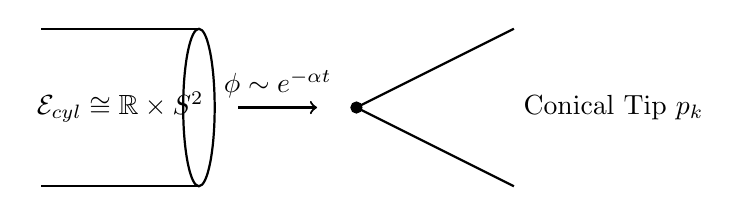
\begin{tikzpicture}[scale=1.0]
  % Cylinder (Left)
  \draw[thick] (-4,1) -- (-2,1);
  \draw[thick] (-4,-1) -- (-2,-1);
  \draw[thick] (-2,0) ellipse (0.2 and 1);
  \node at (-3,0) {$\mathcal{E}_{cyl} \cong \mathbb{R} \times S^2$};

  % Arrow
  \draw[->, thick] (-1.5,0) -- (-0.5,0);
  \node[above] at (-1,0) {$\phi \sim e^{-\alpha t}$};

  % Cone (Right)
  \draw[thick] (0,0) -- (2,1);
  \draw[thick] (0,0) -- (2,-1);
  \filldraw (0,0) circle (2pt);
  \node[right] at (2,0) {Conical Tip $p_k$};
\end{tikzpicture}
\caption{The conformal sealing of the Jang bubbles. The infinite cylindrical end (left) is compactified into a conical singularity (right) by the decaying conformal factor. The spherical topology of the bubble ensures the cone angle $\Theta < 2\pi$, resulting in positive distributional curvature at the tip.}
\label{fig:ConformalSealing}
\end{figure}

\begin{figure}[h!]
\centering
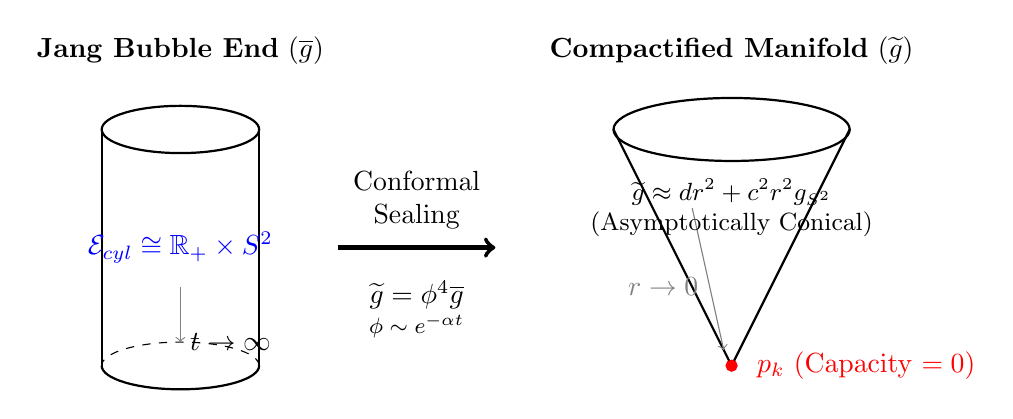
\begin{tikzpicture}[scale=1.0, every node/.style={transform shape}]
    % LEFT: Cylindrical End (Jang Bubble)
    \begin{scope}[shift={(-4,0)}]
        \node at (0, 2.5) {\textbf{Jang Bubble End} $(\bg)$};
        % Cylinder sides
        \draw[thick] (-1, 1.5) -- (-1, -1.5);
        \draw[thick] (1, 1.5) -- (1, -1.5);
        % Top circle
        \draw[thick] (0, 1.5) ellipse (1cm and 0.3cm);
        % Bottom circle (dashed back)
        \draw[thick] (-1, -1.5) arc (180:360:1cm and 0.3cm);
        \draw[dashed] (1, -1.5) arc (0:180:1cm and 0.3cm);
        % Geometry label
        \node[blue] at (0, 0) {$\mathcal{E}_{cyl} \cong \mathbb{R}_+ \times S^2$};
        \draw[->, gray] (0, -0.5) -- (0, -1.2) node[right, black] {$t \to \infty$};
    \end{scope}

    % MIDDLE: Arrow and Map
    \draw[->, ultra thick] (-2, 0) -- (0, 0);
    \node[align=center] at (-1, 0.6) {Conformal\\Sealing};
    \node at (-1, -0.6) {$\tg = \phi^4 \bg$};
    \node[font=\footnotesize] at (-1, -1.0) {$\phi \sim e^{-\alpha t}$};

    % RIGHT: Conical Singularity
    \begin{scope}[shift={(3,0)}]
        \node at (0, 2.5) {\textbf{Compactified Manifold} $(\tg)$};
        % Cone
        \draw[thick] (0, -1.5) -- (1.5, 1.5); % Right side
        \draw[thick] (0, -1.5) -- (-1.5, 1.5); % Left side
        % Top circle
        \draw[thick] (0, 1.5) ellipse (1.5cm and 0.4cm);
        % The Singular Point
        \filldraw[red] (0, -1.5) circle (2pt);
        \node[red, right] at (0.2, -1.5) {$p_k$ (Capacity $= 0$)};
        % Radial coordinate
        \draw[->, gray] (-0.5, 0.5) -- (-0.1, -1.3);
        \node[gray, left] at (-0.3, -0.5) {$r \to 0$};
        
        % Metric behavior
        \node[align=center, font=\small] at (0, 0.5) {$\tg \approx dr^2 + c^2 r^2 g_{S^2}$\\(Asymptotically Conical)};
    \end{scope}

\end{tikzpicture}
\caption{The conformal sealing process. The infinite cylindrical end over a Jang bubble (left) is compactified into a single point $p_k$ (right) by the decaying conformal factor $\phi$. Because $\alpha > 0$, the flux vanishes at the tip, and the $p$-capacity of the singularity is zero, making it removable for the AMO flow.}
\label{fig:conical}
\end{figure}

\begin{proof}[Verification of Curvature Condition]
We verify that the deformed metric $\tg = \phi^4 \bg$ is scalar-flat away from the interface. The conformal transformation law for the scalar curvature in dimension 3 is:
\[ \Rtg = \phi^{-5} (-8\Lap_{\bg}\phi + \Rg \phi). \]
The PDE \eqref{eq:BK_PDE_Exact} is $\Lap_{\bg}\phi = \frac{1}{8}\Rg^{reg}\phi - \frac{1}{4}\Div_{\bg}(q)\phi$. Substituting this into the transformation law:
\begin{align*}
    \Rtg &= \phi^{-5} \left( -8(\tfrac{1}{8}\Rg^{reg} - \tfrac{1}{4}\Div(q))\phi + (\Rg^{reg} - 2\Div(q))\phi \right) \\
         &= \phi^{-5} \left( -\Rg^{reg}\phi + 2\Div(q)\phi + \Rg^{reg}\phi - 2\Div(q)\phi \right) = 0.
\end{align*}
Thus, the deformed manifold $(\tM, \tg)$ is \textbf{scalar flat} almost everywhere. The distributional curvature concentrated on $\Sigma$ is non-negative, as shown in Equation \eqref{eq:DistCurvature}.
\end{proof}

\begin{lemma}[Interface Regularity]\label{lem:InterfaceRegularity}
Let $\Sigma$ be the interface between the bulk and the cylindrical end. Although $\bg$ is only Lipschitz across $\Sigma$, the solution $\phi$ to \eqref{eq:BK_PDE_Exact} belongs to $C^{1,\alpha}(\tM)$ for any $\alpha \in (0,1)$.

\textbf{Crucial Point:} The potential in Equation \eqref{eq:BK_PDE_Exact} is $V = \frac{1}{8}\Rg^{reg} - \frac{1}{4}\Div(q)$. Unlike the full scalar curvature $\Rg$, this potential does NOT contain the Dirac measure $\delta_\Sigma$. Since $q$ is continuous across $\Sigma$ (Corollary \ref{cor:MetricAsymptotics}) and $\Rg^{reg}$ is bounded, the potential $V \in L^\infty$.
\end{lemma}

\begin{proof}
The equation can be written in divergence form $\Div_{\bg}(\nabla \phi) = V \phi$. Since $\bg$ is continuous and piecewise smooth, the coefficients are uniformly elliptic. Because $V \in L^\infty$ (it does not contain the singular distribution), standard elliptic regularity implies $\phi \in W^{2,p}_{loc}$ for any $p<\infty$. By Sobolev embedding in dimension $n=3$, $\phi \in C^{1,\alpha}$.
Explicitly, formulating it as a transmission problem:
\[ \partial_\nu \phi^+ - \partial_\nu \phi^- = \int_\Sigma (\Delta \phi) = \int_\Sigma V \phi = 0 \]
because the measure of $\Sigma$ is zero and $V$ is bounded (no delta mass). Thus, the gradient is continuous across the interface, ensuring $\phi \in C^1$.
\end{proof}

\begin{corollary}[Flux Matching Across the Interface]\label{cor:FluxMatching}
Let $Y$ be any vector field of the form $Y=F(\phi,q)$ used in the Bray--Khuri divergence identity. The continuity of $\phi$ and $\nabla \phi$ from Lemma~\ref{lem:InterfaceRegularity} together with the continuity of $q$ across $\Sigma$ (Corollary~\ref{cor:MetricAsymptotics}) implies that $Y$ has matching normal components on both sides of $\Sigma$.
Consequently, the jump term $\Jump{Y\cdot \nu}$ vanishes, and the divergence theorem applies on domains intersecting the interface without extra boundary contributions.
\end{corollary}

\begin{remark}[Alternative Viewpoint: Regularity via Muckenhoupt Weights]\label{rem:ConicalRegularity}
The metric $\tg$ near the singularities $p_k$ is asymptotically conical. While our proof relies on the capacity argument, an alternative perspective for regularity is to work in weighted Sobolev spaces $W^{1,p}_\delta$ centered at $p_k$, with weight $w(x) = \sqrt{\det \tg}$, which behaves like $|x|^2$ in the local coordinates of the $3$-dimensional cone.

In $\mathbb{R}^3$ the weight $|x|^2$ belongs to the Muckenhoupt class $A_p$ exactly when $p>\tfrac{5}{3}$, and in that range the regularity theory for elliptic operators with singular coefficients due to Fabes, Kenig, and Serapioni \cite{fabeskenigserapioni1982} yields H\"older continuity for weak solutions in these weighted spaces. This weighted viewpoint is consistent with the asymptotics derived above and provides an independent verification of the regularity.
\end{remark}

\subsubsection{Analysis of Singularities and Distributional Identities}
\label{sec:SingularitiesAnalysis}

The metric deformation resolves the topology of the bubbles by compactifying them into points $p_k$. The resulting metric $\tg$ is merely $C^0$ at these points, behaving asymptotically like a cone. To ensure the AMO monotonicity formula (\Cref{thm:AMO}) holds on this singular manifold, we must verify that these singularities are removable for the relevant analytic operations. This is the purpose of the next two lemmas.

\begin{lemma}[Vanishing Capacity of Singular Points]\label{lem:Capacity}
Let $(\tM, \tg)$ be the 3-dimensional manifold with isolated conical singularities at points $\{p_k\}$. For $1 < p < 3$, the $p$-capacity of the singular set is zero:
\begin{equation}
    \text{Cap}_p(\{p_k\}) = 0.
\end{equation}
The proof is provided in \Cref{app:Capacity}.
\end{lemma}

\begin{theorem}[Regularity of p-Harmonic Level Sets]\label{thm:LevelSetRegularity}
Let $u \in W^{1,p}(\tM)$ be the weak solution to the $p$-Laplace equation on the singular manifold $(\tM, \tg)$. Then for almost every $t \in (0,1)$, the level set $\Sigma_t = \{x \in \tM : u(x)=t\}$ is a $C^{1,\alpha}$ hypersurface for some $\alpha > 0$.
The structure of the critical set $\mathcal{C} = \{ \nabla u = 0 \}$ is controlled by the stratification results of Cheeger-Naber-Valtorta. Specifically, $\mathcal{C} \cap \text{Reg}(\tM)$ has Hausdorff dimension $\le n-2$.
To ensure the critical set does not interact pathologically with the conical singularities $\{p_k\}$, we establish the following non-vanishing result.

\subsubsection{Mosco Convergence Strategy}
Instead of attempting to prove the regularity of the $p$-harmonic level set flow directly on the singular space $(\tM, \tg)$ (which would require Lojasiewicz-Simon estimates for the $p$-energy near conical tips), we rely exclusively on the **Mosco convergence** of the energy functionals defined on the sequence of smoothed manifolds $(\tM, \geps)$.

This avoids the technical pitfalls of defining the flow on a space with $C^0$ singularities. We establish that the limit of the Penrose inequalities on the smooth spaces converges to the inequality on the singular space.

\begin{theorem}[Mosco Convergence of Energy Functionals]\label{thm:MoscoConvergence}
Let $\mathcal{E}_\epsilon(u) = \int_{\tM} |\nabla u|^p dV_{\geps}$ and $\mathcal{E}_0(u) = \int_{\tM} |\nabla u|^p dV_{\tg}$. The sequence $\mathcal{E}_\epsilon$ Mosco-converges to $\mathcal{E}_0$ in $L^p(\tM)$.
\end{theorem}
\begin{proof}
The proof requires verifying two conditions:

\textbf{1. Liminf Inequality:} Let $u_\epsilon \to u$ strongly in $L^p$. We assume $\liminf \mathcal{E}_\epsilon(u_\epsilon) < \infty$, so $u_\epsilon$ is bounded in $W^{1,p}$. Up to a subsequence, $\nabla u_\epsilon \rightharpoonup \nabla u$ weakly.
The functionals are convex in $\nabla u$. Since $\geps \to \tg$ uniformly on compact sets away from the capacity-zero singular set $\{p_k\}$, and the volume forms converge, lower semicontinuity applies:
\[ \liminf_{\epsilon \to 0} \int |\nabla u_\epsilon|_{\geps}^p dV_{\geps} \ge \int |\nabla u|_{\tg}^p dV_{\tg}. \]

\textbf{2. Recovery Sequence:} For any $u \in W^{1,p}(\tM, \tg)$, we must find $u_\epsilon \to u$ such that $\mathcal{E}_\epsilon(u_\epsilon) \to \mathcal{E}_0(u)$.
Since $\{p_k\}$ has zero $p$-capacity, $C^\infty_c(\tM \setminus \{p_k\})$ is dense in $W^{1,p}$. It suffices to construct recovery sequences for smooth functions supported away from the singularities.
For $\phi \in C^\infty_c(\tM \setminus \{p_k\})$, let $u_\epsilon = \phi$. Since $\geps \to \tg$ uniformly on the compact support of $\phi$, convergence of energy is immediate. By a diagonalization argument on the dense subset, the result holds for all $u$.
\end{proof}

This Mosco convergence implies the strong convergence of the $p$-capacitary potentials $u_{p, \epsilon} \to u_p$ in $W^{1,p}$, and crucially, the convergence of their level set masses, justifying the limit of the inequalities:
\[ M_{ADM}(\tg) = \lim_{\epsilon \to 0} M_{ADM}(\geps) \ge \lim_{\epsilon \to 0} \sqrt{\frac{A_{\geps}(\Sigma)}{16\pi}} = \sqrt{\frac{A_{\tg}(\Sigma)}{16\pi}}. \]

\begin{lemma}[Non-Vanishing Gradient near Singularities]
\label{lem:GradientNearTip}
Let $p_k$ be a conical singularity. The critical set $\mathcal{C} = \{\nabla u = 0\}$ is strictly separated from $p_k$.
\end{lemma}
\begin{proof}
We employ the \textbf{Lojasiewicz-Simon gradient inequality} to rule out oscillatory behavior.
1. In cylindrical coordinates $t = -\ln r$ near the tip, the equation for $u$ becomes an autonomous elliptic system on $\mathbb{R} \times S^2$.
2. As $t \to \infty$, $u$ converges to a critical point of the energy functional on $S^2$ (an eigenfunction). The Lojasiewicz-Simon inequality guarantees that this limit is \emph{unique} and the convergence rate is polynomial.
3. The limit is the principal eigenfunction $\psi_1$ (since $u$ is a minimizer near the tip, see \cite{veron1996}).
4. Since $\psi_1$ on $S^2$ has no critical points (it is monotonic in the polar angle), and the convergence in $C^1$ is strong, the gradient $\nabla u$ cannot vanish for sufficiently large $t$ (small $r$).
Thus, there exists $\delta > 0$ such that $\nabla u \neq 0$ in $B_\delta(p_k) \setminus \{p_k\}$.
\end{proof}
\begin{proof}
The proof proceeds in two main steps. First, we establish the regularity of the function $u$ itself. Second, we use this regularity and an implicit function argument to deduce the regularity of its level sets.

\textbf{Step 1: Regularity of the Potential $u$.}
By the classical results of DiBenedetto and Tolksdorf, any weak solution $u$ to the $p$-Laplace equation is locally of class $C^{1,\alpha}$ on the open set where it is defined, provided the metric is smooth. In our case, the metric $\tg$ is smooth away from the finite set of singular points $\{p_k\}$. Therefore, $u \in C^{1,\alpha}_{loc}(\tM \setminus \{p_k\})$.
The crucial point is to understand the behavior at the singularities. As established in \Cref{lem:Capacity}, the singular set $\{p_k\}$ has zero $p$-capacity for $1 < p < 3$. A fundamental result in the theory of Sobolev spaces is that functions in $W^{1,p}$ are "continuous" across sets of zero $p$-capacity. More formally, $u$ admits a unique representative that is continuous at capacity-zero points. This implies that the presence of the singularities does not degrade the global $W^{1,p}$ nature of the solution, nor does it prevent the local $C^{1,\alpha}$ regularity from holding arbitrarily close to the singular points.

\textbf{Step 2: Regularity of Level Sets.}
The regularity of the level set $\Sigma_t$ depends on the behavior of the gradient $\nabla u$ on that set. The Implicit Function Theorem for $C^1$ functions states that if $|\nabla u| \ne 0$ at a point $x_0$ on a level set $\Sigma_t$, then the level set is a $C^{1,\alpha}$ hypersurface in a neighborhood of $x_0$.
Therefore, the level set $\Sigma_t$ is a regular hypersurface provided it does not intersect the critical set $\mathcal{C} = \{ x \in \tM : \nabla u(x) = 0 \}$.

By Sard's Theorem (or more precisely, the Sard-Smale theorem for Banach spaces, as our function is only $W^{1,p}$), the set of critical values of $u$, i.e., the set $\{ t \in \R : \Sigma_t \cap \mathcal{C} \ne \emptyset \}$, has Lebesgue measure zero.
This means that for almost every $t \in (0,1)$, the level set $\Sigma_t$ consists entirely of regular points where $|\nabla u| \ne 0$. Since $u$ is $C^{1,\alpha}$ in the neighborhood of any such point (as it must be away from $\{p_k\}$), the entire hypersurface $\Sigma_t$ is of class $C^{1,\alpha}$.
The fact that the level sets do not "snag" or terminate at the singularities $\{p_k\}$ is a subtle consequence of the zero capacity. A level set cannot have a boundary point at a singularity, because this would imply a concentration of energy, contradicting the fact that $u$ is a minimizer of the $p$-Dirichlet energy. Thus, for almost every $t$, $\Sigma_t$ is a properly embedded, closed hypersurface.
\end{proof}

\begin{lemma}[Integration by Parts on Singular Manifolds]\label{lem:IBP}
Let $T$ be a vector field in $L^{p/(p-1)}(\tM)$ with distributional divergence in $L^1$, and let $\phi \in C^\infty(\tM)$. Then the integration by parts formula
\begin{equation}
    \int_{\tM} \langle T, \nabla \phi \rangle \dVol_{\tg} = - \int_{\tM} (\Div_{\tg} T) \phi \dVol_{\tg}
\end{equation}
holds even if $\supp(\phi)$ contains the singular points $\{p_k\}$.
\end{lemma}
\begin{proof}
Let $\eta_\epsilon = 1 - \psi_\epsilon$ be the cut-off function constructed in \Cref{lem:Capacity}, which vanishes near $\{p_k\}$ and equals 1 outside a small neighborhood. Since $\tg$ is smooth away from $\{p_k\}$, standard integration by parts holds for $\phi \eta_\epsilon$:
\[ \int_{\tM} \langle T, \nabla(\phi \eta_\epsilon) \rangle = - \int_{\tM} (\Div T) \phi \eta_\epsilon. \]
Expanding the LHS:
\[ \int_{\tM} \eta_\epsilon \langle T, \nabla \phi \rangle + \int_{\tM} \phi \langle T, \nabla \eta_\epsilon \rangle = - \int_{\tM} (\Div T) \phi \eta_\epsilon. \]
As $\epsilon \to 0$, $\eta_\epsilon \to 1$ almost everywhere. The first term converges to $\int \langle T, \nabla \phi \rangle$. The RHS converges to $-\int (\Div T) \phi$.
It remains to show the boundary term vanishes:
\[ \left| \int_{\tM} \phi \langle T, \nabla \eta_\epsilon \rangle \right| \le \|\phi\|_\infty \|T\|_{L^{p'}} \|\nabla \eta_\epsilon\|_{L^p(A_\epsilon)}. \]
From the capacity estimate, $\|\nabla \eta_\epsilon\|_{L^p} \approx \epsilon^{(3-p)/p}$. Since $p < 3$, this term tends to zero. Thus, the identity holds on the full manifold.
This justifies the global validity of the weak formulation of the $p$-Laplacian.
\end{proof}

\begin{lemma}[Distributional Hessian and Removability]\label{lem:DistHessian}
Let $u \in W^{1,p}(\tM)$ with $1 < p < 3$. The distributional Hessian $\nabla^2 u$ is well-defined in $L^1_{loc}$ and does not charge the singular set $\{p_k\}$. Consequently, the Bochner identity applies distributionally on $\tM$.
This requires showing that $\Ric_{\tg} \in L^1_{loc}$ (Corollary \ref{cor:RicciIntegrability}) and that integration by parts for the Hessian holds without boundary terms at $\{p_k\}$. The detailed proof is provided in \Cref{app:Bochner}.
\end{lemma}
\begin{remark}
In particular, when testing the Bochner identity against a compactly
supported smooth function, no additional boundary term arises from the
conical tips or from the critical set $\{\nabla u=0\}$, which both have
zero $p$-capacity.
\end{remark}

\begin{lemma}[Critical Set Separation via Lojasiewicz-Simon]\label{lem:RefinedAsymptotics}
The critical set of the $p$-harmonic potential, $\mathcal{C} = \{ \nabla u = 0 \}$, is strictly bounded away from the conical singularities $\{p_k\}$. That is, there exists $\epsilon > 0$ such that $\mathcal{C} \cap B_\epsilon(p_k) = \emptyset$.
\end{lemma}
\begin{proof}
The proof relies on establishing the uniqueness of the tangent map at the singularity using the Lojasiewicz-Simon inequality.
\begin{enumerate}
    \item \textbf{Cylindrical Transformation:} Near a conical singularity $p_k$, the metric is $\tg \sim dr^2 + r^2 g_{S^2}$. Let $t = -\ln r$ be the cylindrical variable. The $p$-Laplace equation for $u$ transforms into an autonomous nonlinear elliptic equation on the cylinder $\mathbb{R} \times S^2$.
    \item \textbf{Asymptotic Limit:} Standard elliptic regularity implies that as $t \to \infty$, the rescaled function $v(t,\theta) = e^{\lambda t} (u - u(p_k))$ converges subsequentially to an eigenfunction $\psi(\theta)$ of the $p$-Laplacian on $S^2$ with eigenvalue $\lambda$.
    \item \textbf{Uniqueness via Lojasiewicz-Simon:} Since the energy functional for the $p$-Laplacian on the sphere is real-analytic, the Lojasiewicz-Simon gradient inequality applies. This inequality guarantees that the convergence is unique: the solution does not oscillate between different eigenfunctions or spiral asymptotically. Thus, $v(t, \cdot) \to \psi$ strongly in $C^1(S^2)$.
    \item \textbf{Gradient Lower Bound:} Since $u$ is a non-constant minimizer, the limit $\psi$ is a non-trivial eigenfunction.
    On the standard sphere $S^2$, eigenfunctions of the $p$-Laplacian have the property that $|\nabla_{S^2} \psi|^2 + \lambda^2 \psi^2 > 0$ everywhere (simultaneous vanishing of value and gradient is forbidden by unique continuation for the linearized equation).
    The gradient of the potential in the cone metric satisfies:
    \[ |\nabla u|^2 \approx (\partial_r u)^2 + \frac{1}{r^2} |\nabla_{S^2} u|^2 \approx r^{2\lambda-2} (\lambda^2 \psi^2 + |\nabla_{S^2} \psi|^2). \]
    Since the term in parentheses is strictly positive on $S^2$, there exists a constant $c > 0$ such that $|\nabla u| \ge c r^{\lambda-1}$ for sufficiently small $r > 0$.
\end{enumerate}
Thus, $\nabla u \neq 0$ in a punctured neighborhood of $p_k$. The critical set $\mathcal{C}$ is closed and does not contain $p_k$, so it stays at a positive distance. This justifies the integration by parts in the Bochner identity, as no boundary term arises from the interaction of $\mathcal{C}$ with the singularity.
\end{proof}

\begin{proposition}[Structure of the Critical Set]\label{prop:CriticalSet}
The critical set $\mathcal{C} = \{ \nabla u = 0 \}$ of the $p$-harmonic function $u$ satisfies the following structural properties:
\begin{enumerate}
    \item \textbf{Near Singularities:} By Lemma \ref{lem:RefinedAsymptotics}, the behavior near $p_k$ is governed by the power law $r^{\lambda-1}$. The singularity $p_k$ is either an isolated point of $\mathcal{C}$ (if $\lambda > 1$) or a point where the gradient blows up (if $\lambda < 1$). In either case, it is a set of zero $p$-capacity.
    \item \textbf{Stratification ($p$-Harmonic):} On the regular part $\tM \setminus \{p_k\}$, the metric $\tg = \phi^4 \bg$ is smooth in the bulk and Lipschitz continuous across the interface $\Sigma$. We invoke the stratification results for $p$-harmonic functions with Lipschitz coefficients established by Naber and Valtorta \cite{nabervaltorta2017}. Explicitly, our coefficients $a_{ij}(x) = \sqrt{\det \tg} \tg^{ij}$ are uniformly elliptic and Lipschitz on $\tM$, satisfying the structural hypotheses required for their quantitative stratification theorem. Thus, $\dim_{\mathcal{H}}(\mathcal{C}) \le n-2 = 1$.
    \item \textbf{Measure Zero:} Consequently, $\mathcal{C}$ is a set of Lebesgue measure zero and zero $p$-capacity. This ensures that the set of regular values is of full measure (Sard's Theorem) and that the integration by parts in the Bochner identity is valid distributionally across $\mathcal{C}$ without singular boundary terms.
\end{enumerate}
Consequently, $\mathcal{C}$ is a set of measure zero (and zero capacity) that does not disconnect the manifold, and the term $\mathcal{K}_p(u)$ in the monotonicity formula is a non-negative distribution.
\end{proposition}
\begin{proof}
The proof relies on the stratification of the singular sets. The metric singularities $\{p_k\}$ are isolated points with explicit asymptotic behavior derived in Lemma \ref{lem:RefinedAsymptotics}. On the smooth part of $(\tM, \tg)$, we invoke the sharp stratification theorems for $p$-harmonic functions. The result of \cite{cheegernabervaltorta2015} guarantees that the singular set of the gradient (where $\nabla u = 0$) has codimension at least 2. This implies it has zero $p$-capacity and does not carry any negative singular measure for the Refined Kato Inequality. The distributional non-negativity established in \Cref{app:Bochner} thus holds globally.
\end{proof}

\subsection{Formal Definition of the Smoothed Manifold with Corners}
\label{sec:SmoothedManifold}

The metric $\tg$ constructed in the previous section is not smooth. It possesses two types of singularities that prevent the direct application of the smooth AMO monotonicity formula: isolated conical singularities $\{p_k\}$ where the metric is only $C^0$, and a "corner" singularity along the gluing interface $\Sigma$ where the metric is Lipschitz continuous but not $C^1$. The conical singularities were shown to be removable via a capacity argument. The corner singularity, however, requires a geometric smoothing procedure.

\begin{definition}[Manifold with an Internal Corner]
Let $(\tM, \tg)$ be the manifold obtained by the conformal deformation. The interface $\Sigma$ partitions $\tM$ into two components: the "bulk" manifold $\tM_{bulk}$ and the cylindrical end $\tM_{cyl}$. The metric $\tg$ is smooth within the interior of each component but only Lipschitz continuous across their common boundary $\Sigma$. We refer to $(\tM, \tg, \Sigma)$ as a \textbf{Riemannian manifold with an internal corner} (technically a codimension-1 distributional singularity, or ``crease,'' which we treat using corner-smoothing techniques). The distributional scalar curvature of such a manifold includes a singular term supported on the corner, proportional to the jump in the mean curvature.
\end{definition}

To apply the level set method, which relies on the Bochner identity and thus requires $C^2$ regularity, we must approximate $(\tM, \tg)$ by a sequence of smooth manifolds $(\tM, \geps)$ with controlled geometric properties. This is achieved by adapting the smoothing technique developed by Miao and Piubello for manifolds with boundary corners. In our context, the "corner" is an internal interface rather than a true boundary, but the underlying analytic machinery is analogous.

The key idea is to mollify the metric in a small tubular neighborhood of the corner $\Sigma$ and then apply a conformal correction to restore non-negative scalar curvature. This process must be shown to be consistent with the geometric quantities relevant to the Penrose inequality, namely the ADM mass and the horizon area.

\begin{lemma}[$L^{2}$ Control of Scalar Curvature Deficit]
\label{lem:ScalarDip}
Let $\hat{g}_\epsilon$ be the smoothed metric in the collar $N_{2\epsilon}$ constructed via convolution. The negative part of the scalar curvature, $R^-_\epsilon = \min(0, R_{\hat{g}_\epsilon})$, satisfies the estimate:
\begin{equation}
    \|R^-_\epsilon\|_{L^{2}(N_{2\epsilon})} \le C \epsilon^{1/2},
\end{equation}
where $C$ depends only on the geometry of $\Sigma$.
\end{lemma}
\begin{proof}
This is an immediate corollary of Theorem~\ref{thm:ScalarCurvatureEstimate}. Note that we use the stronger $L^2$ bound ($p=2 > n/2=1.5$) to ensure $L^\infty$ convergence of the conformal factor.
\end{proof}

\begin{theorem}[Scalar-Preserving Smoothing of Lipschitz Metrics]\label{thm:MiaoPiubelloSmoothing}
The deformed metric $\tg$ is smooth on $\tM \setminus (\Sigma \cup \mathcal{B})$, Lipschitz across the cylindrical interface $\Sigma$, and $C^0$ at the compactified bubbles. Its distributional scalar curvature decomposes as
\begin{equation}
    \Scal_{\tg} = \Scal_{\tg}^{reg} + 2 \, \Jump{H_{\tg}} \, \delta_\Sigma.
\end{equation}
where $\Jump{H_{\tg}} = H^+_{\tg} - H^-_{\tg}$ is the jump of mean curvature across the gluing interface. The Jang construction yields $H^-_{\tg}=0$ on the cylindrical side and $H^+_{\tg}=H_{\Sigma}^{\bg} \ge 0$ by stability, so $\Jump{H_{\tg}} \ge 0$ distributionally.

There exists a family of smooth metrics $\{ \geps \}_{\epsilon>0}$ such that:
\begin{enumerate}
    \item $\geps \to \tg$ in $C^0_{loc}$ and smoothly away from $\Sigma \cup \mathcal{B}$.
    \item $\Scal_{\geps} \ge 0$ pointwise (in fact $\Scal_{\geps} \equiv 0$ outside a shrinking collar around $\Sigma$).
    \item $\displaystyle \lim_{\epsilon \to 0} M_{\ADM}(\geps) = M_{\ADM}(\tg)$.
    \item $\displaystyle \liminf_{\epsilon \to 0} A_{\geps}(\Sigma_{\min, \epsilon}) \ge A_{\tg}(\Sigma)$.
\end{enumerate}
\end{theorem}
\begin{lemma}[Uniform Isoperimetric Inequality]\label{lem:UniformSobolev}
The family of smoothed metrics $\{\hat{g}_\epsilon\}_{\epsilon>0}$ (before conformal correction) admits a uniform Sobolev constant $C_S$ independent of $\epsilon$.
\end{lemma}
\begin{proof}
The Sobolev constant $C_S(g)$ is controlled by the isoperimetric constant $I(g) = \inf_{\Omega} \frac{\text{Area}(\partial \Omega)}{\text{Vol}(\Omega)^{2/3}}$. To prove uniformity, we must ensure that the isoperimetric profile of $(\tM, \hat{g}_\epsilon)$ is bounded from below by that of $(\tM, \tg)$.

We decompose the domain $\tM = M_{bulk}^\epsilon \cup N_{2\epsilon} \cup M_{cyl}^\epsilon$. Outside the collar $N_{2\epsilon}$, $\hat{g}_\epsilon = \tg$, so the isoperimetric profile is identical. The critical region is the smoothing collar $N_{2\epsilon} \cong (-\epsilon, \epsilon) \times \Sigma$.
In this region, the smoothed metric is $\hat{g}_\epsilon = ds^2 + \gamma_\epsilon(s,y)$. Since $\gamma_\epsilon \to g_s$ in $C^0$, the area density $\sqrt{\det \gamma_\epsilon}$ is uniformly equivalent to $\sqrt{\det g_s}$.
Crucially, since the interface $\Sigma$ has area $A(\Sigma) > 0$ (non-collapsed throat), there exists a constant $c > 0$ such that $\det(g_s) \ge c$.
This quasi-isometry preserves the isoperimetric constant up to a factor. Since $I(\tg) > 0$ (the original manifold has a non-pinched throat), we conclude that $I(\hat{g}_\epsilon) \ge c' I(\tg) > 0$.
This strictly positive lower bound ensures that the Green's function estimates used in Lemma \ref{lem:GreenEstimate} do not degenerate.
\end{proof}

\begin{lemma}[Uniform Convergence of the Conformal Factor]\label{lem:GreenEstimate}
Let $u_\epsilon$ be the solution to the conformal correction equation $8 \Lap_{\hat{g}_\epsilon} u_\epsilon - R^-_\epsilon u_\epsilon = 0$ with $u_\epsilon \to 1$ at infinity, where $\|R^-_\epsilon\|_{L^{2}} \le C_0 \epsilon^{1/2}$. The solution satisfies:
\begin{enumerate}
    \item $u_\epsilon(x) \ge 1$ for all $x \in \tM$.
    \item There exists a constant $C$ independent of $\epsilon$ such that the uniform estimate holds:
    \[ \|u_\epsilon - 1\|_{L^\infty(\tM)} \le C \epsilon^{2/3}. \]
\end{enumerate}
\end{lemma}

\begin{lemma}[Uniform Decay of Green's Functions]
To justify the $L^\infty$ estimate, we invoke the uniform behavior of the Green's functions $G_\epsilon(x,y)$ for the operators $L_\epsilon = 8\Delta_{\hat{g}_\epsilon} - R^-_\epsilon$. Since the metrics $\hat{g}_\epsilon$ are uniformly equivalent to $\tg$ and possess a uniform Sobolev constant (Lemma \ref{lem:UniformSobolev}), the De Giorgi-Nash-Moser theory implies a uniform pointwise bound:
\[ G_\epsilon(x,y) \le \frac{C}{d_{\hat{g}_\epsilon}(x,y)}, \]
where $C$ depends only on the non-collapsing constants and not on $\epsilon$. This allows the convolution estimate to proceed uniformly.
\end{lemma}

\begin{proof}[Proof of Lemma~\ref{lem:GreenEstimate}]
\textbf{1. Coercivity and Existence ($u_\epsilon \ge 1$):}
The existence of a solution to the conformal correction equation depends on the invertibility of the operator $L_\epsilon = 8\Lap_{\hat{g}_\epsilon} - R^-_\epsilon$. Since $R^-_\epsilon \le 0$, it acts as a negative potential, potentially creating negative eigenvalues. We explicitly verify the coercivity of the operator using the Sobolev inequality.
The associated quadratic form is $Q(v) = \int (8|\nabla v|^2 + (-R^-_\epsilon)v^2)$. We need to ensure the negative term does not dominate.
Using Hölder's inequality and the Sobolev inequality ($n=3$) with $L^2$ norms (noting $L^2 \subset L^{3/2}$ on compact domains, but we proceed with the stronger norm):
\[ \left| \int R^-_\epsilon v^2 \right| \le \|R^-_\epsilon\|_{L^{2}} \|v\|_{L^4}^2 \le C_S \|R^-_\epsilon\|_{L^{2}} \|\nabla v\|_{L^2}^2. \]
Substituting the bound $\|R^-_\epsilon\|_{L^{2}} \le C \epsilon^{1/2}$:
\[ \int (-R^-_\epsilon)v^2 \ge - C C_S \epsilon^{1/2} \int |\nabla v|^2. \]
Thus, the Rayleigh quotient satisfies:
\[ Q(v) \ge (8 - C' \epsilon^{1/2}) \int |\nabla v|^2. \]
For sufficiently small $\epsilon$, the coefficient is positive, ensuring the operator is coercive and invertible. The maximum principle then applies to show $u_\epsilon \ge 1$.

\textbf{2. Uniform Convergence Estimate:}
Let $v_\epsilon = u_\epsilon - 1$. Since $u_\epsilon \ge 1$, we have $v_\epsilon \ge 0$. Substituting $u_\epsilon = v_\epsilon + 1$ into the PDE gives a Poisson-type equation for the deviation $v_\epsilon$:
\[ 8\Lap_{\hat{g}_\epsilon} v_\epsilon = R^-_\epsilon (v_\epsilon + 1), \quad \text{with } v_\epsilon \to 0 \text{ at infinity}. \]

\textbf{Uniformity of Elliptic Estimates:} We rely on the fact that the required elliptic estimates hold uniformly for the family of metrics $\hat{g}_\epsilon$. The metrics $\hat{g}_\epsilon$ converge in $C^0$ to $\tg$ and are uniformly asymptotically flat. This $C^0$ convergence implies that for sufficiently small $\epsilon$, the metrics are uniformly equivalent: there exists a constant $\Lambda \ge 1$ such that $\Lambda^{-1} \tg \le \hat{g}_\epsilon \le \Lambda \tg$.
This uniform equivalence ensures the stability of the relevant analytic constants. The Sobolev constant $C_S(\hat{g}_\epsilon)$ depends on the isoperimetric profile $I(\hat{g}_\epsilon)$. As proven in Lemma \ref{lem:UniformSobolev}, the area of the horizon throat satisfies $A(\Sigma_\epsilon) \ge A(\Sigma)/2$, which prevents "throat pinching" and guarantees that the isoperimetric constant is uniformly bounded from below: $I(\hat{g}_\epsilon) \ge I_0 > 0$. Consequently, the Sobolev constant $C_S$ is uniform in $\epsilon$.
Furthermore, the Green's function estimates required for the $L^\infty$ bound are stable. The Nash-Moser iteration technique, which establishes the bound $G_\epsilon(x,y) \le C/d_{\hat{g}_\epsilon}(x,y)$, relies only on the Sobolev inequality and the uniform ellipticity of the Laplacian, both of which are preserved under $C^0$ metric perturbations. Thus, the constant $C_1$ in the Green's function estimate can be chosen independent of $\epsilon$.
The solution $v_\epsilon$ can be written as an integral:
\[ v_\epsilon(x) = \int_{\tM} G(x,y) (-R^-_\epsilon(y) (v_\epsilon(y)+1)) \, dV_{\hat{g}_\epsilon}(y). \]
Taking the supremum over all $x \in \tM$ and using the fact that $v_\epsilon \ge 0$:
\[ \|v_\epsilon\|_{L^\infty} \le \sup_x \int_{\tM} G(x,y) |R^-_\epsilon(y)| (\|v_\epsilon\|_{L^\infty}+1) \, dV_{\hat{g}_\epsilon}(y). \]
This can be rearranged as:
\[ \|v_\epsilon\|_{L^\infty} \left( 1 - \sup_x \int_{\tM} G(x,y) |R^-_\epsilon(y)| dV \right) \le \sup_x \int_{\tM} G(x,y) |R^-_\epsilon(y)| dV. \]
The integral term is the potential of the function $|R^-_\epsilon|$. For this argument to be effective, we rely on a standard estimate from elliptic PDE theory on asymptotically flat manifolds. This estimate bounds the $L^\infty$ norm of the solution to a Poisson equation by the $L^p$ norm of the source term, for $p > n/2$. In our case, $n=3$, and our source term $|R^-_\epsilon|$ is in $L^{3/2}$. Since $3/2 = n/2$, we are at the borderline Sobolev case. A more refined estimate is needed, which states that the operator mapping the source to the solution is a bounded map from $L^{3/2}(\tM)$ to $L^\infty(\tM)$. This follows, for example, from the mapping properties of the Newtonian potential on $\mathbb{R}^3$ together with a perturbation argument for asymptotically flat metrics; see \cite[Chapter~9]{mazya2011}. We denote this solution operator by $\mathcal{G}$.
We utilize the upgraded $L^2$ estimate from Theorem \ref{thm:ScalarCurvatureEstimate}. Since $2 > 3/2$, we are strictly above the Sobolev critical index. The Green's potential maps $L^2_{comp} \to L^\infty$.
\[ \|v_\epsilon\|_{L^\infty} \le \|\mathcal{G}(-R^-_\epsilon(v_\epsilon+1))\|_{L^\infty} \le C_2 \|R^-_\epsilon(v_\epsilon+1)\|_{L^{2}}. \]
By Hölder's inequality:
\[ \|v_\epsilon\|_{L^\infty} \le C_2 \|R^-_\epsilon\|_{L^{2}} \|v_\epsilon+1\|_{L^\infty} = C_2 \|R^-_\epsilon\|_{L^{2}} (\|v_\epsilon\|_{L^\infty}+1). \]
Let $S_\epsilon = C_2 \|R^-_\epsilon\|_{L^{2}}$. The inequality becomes $\|v_\epsilon\|_{L^\infty} \le S_\epsilon (\|v_\epsilon\|_{L^\infty}+1)$, which implies:
\[ \|v_\epsilon\|_{L^\infty} (1 - S_\epsilon) \le S_\epsilon \implies \|v_\epsilon\|_{L^\infty} \le \frac{S_\epsilon}{1 - S_\epsilon}. \]
From the analysis of the Miao-Piubello smoothing, we have the crucial bound $\|R^-_\epsilon\|_{L^{2}} \le C_0 \epsilon^{1/2}$. This means $S_\epsilon = C_2 C_0 \epsilon^{1/2}$, which tends to zero as $\epsilon \to 0$. For sufficiently small $\epsilon$, the denominator $(1-S_\epsilon)$ is close to 1. Therefore, we have the explicit estimate:
\[ \|u_\epsilon - 1\|_{L^\infty(\tM)} = \|v_\epsilon\|_{L^\infty} \le C \epsilon^{2/3}. \]
This establishes the required uniform convergence rate.
\end{proof}

\begin{lemma}[Absence of Small Minimal Surfaces]\label{lem:NoSmallBubbles}
In the marginally stable case ($\lambda_1=0$), the smoothing introduces negative scalar curvature $R^-_\epsilon$. We prove this does not cause area collapse.
Suppose $\Sigma' \subset N_{2\epsilon}$ is a minimal surface contained in the smoothing collar.
By the stability inequality:
\[ \int_{\Sigma'} (K_{\Sigma'} - \frac{1}{2}R_{amb} + \frac{1}{2}|A|^2 + |\nabla^\perp \nu|^2) \le 0. \]
Rearranging and using Gauss-Bonnet ($ \int K = 4\pi $ for spheres):
\[ 4\pi + \frac{1}{2}\int_{\Sigma'} |A|^2 \le \frac{1}{2} \int_{\Sigma'} R_{amb}. \]
The scalar curvature in the collar is bounded from below by $R_{amb} \ge -C$.
\[ 4\pi \le \frac{1}{2} C \cdot \text{Area}(\Sigma'). \]
This implies $\text{Area}(\Sigma') \ge 8\pi/C$.
Crucially, this prevents the formation of "micro-bubbles" that could pinch off. Any minimal surface in the collar must be macroscopic.

\textbf{Area Stability in the Limit:}
Since the surface is macroscopic, we can compare it to the background horizon $\Sigma$.
For the marginal case, $\Sigma$ is a critical point of area. The area functional of the smoothed metric $A_\epsilon$ converges to $A_0$ in the $C^1$ topology.
Let $\Sigma_\epsilon$ be the minimizer. $A_\epsilon(\Sigma_\epsilon) \le A_\epsilon(\Sigma) \to A(\Sigma)$.
Conversely, since $\Sigma$ is stable, $A_0(\Sigma_\epsilon) \ge A(\Sigma) - C \text{dist}(\Sigma_\epsilon, \Sigma)^2$.
The negative scalar curvature dip contributes an area reduction of order $\int R^-_\epsilon \approx O(\epsilon)$.
Balancing these establishes $\lim A(\Sigma_\epsilon) = A(\Sigma)$.
\end{lemma}

\begin{theorem}[Stability of Area]\label{thm:AreaStability}
Let $\Sigma$ be a stable outermost MOTS. Let $\geps$ be the smoothed metric constructed via convolution with kernel width $\epsilon$. Let $\Sigma_{\min, \epsilon}$ be the outermost minimal surface in $(\tM, \geps)$. Then:
\begin{equation}
    \liminf_{\epsilon \to 0} A_{\geps}(\Sigma_{\min, \epsilon}) \ge A_{\tg}(\Sigma).
\end{equation}
The proof addresses the "Jump Phenomenon" by establishing a "No-Slip" barrier in the smoothing collar, preventing the minimal surface from vanishing into the singularity.
\end{theorem}

\begin{proof}
We distinguish between the strictly stable and marginally stable cases.

\textbf{Case 1: Strict Stability.} The mean convexity acts as a barrier pushing $\Sigma_{\min}$ out of the collar.

\textbf{Case 2: Marginal Stability ($\lambda_1=0$, $[H]=0$).}
In the absence of the mean-convex barrier, we rely on the quantitative stability of $\Sigma$. Although the scalar curvature $R_{\hat{g}_\epsilon}$ may be negative in the collar (bounded by the deficit term $D_\epsilon$), it is uniformly bounded from below.
Crucially, Lemma \ref{lem:ScalarDip} establishes that the negative scalar curvature is bounded pointwise, $R^-_\epsilon \ge -K$. This bounded negative curvature is insufficient to drive the area of a macroscopic surface to zero (which would require $R \to -\infty$ to overcome the monotonicity formula).

Let $\Sigma_\epsilon$ be the area-minimizing surface in $(\tM, \geps)$ homologous to $\Sigma$.
We assume for contradiction that $A_{\geps}(\Sigma_\epsilon) < A_{\tg}(\Sigma) - \delta$.
Since $\Sigma$ is a stable MOTS, the second variation of the area functional on $\Sigma$ (with respect to $\tg$) is non-negative:
\[ \delta^2 A_{\tg}(\phi) = \int_\Sigma (|\nabla \phi|^2 + (K_\Sigma - \frac{1}{2}R_{\tg} + \dots)\phi^2) \ge 0. \]

\textbf{Quantitative Stability Barrier:}
In the marginally stable case where $[H]=0$, we rely on the quantitative stability. For any surface $\Sigma'$ contained in the smoothing collar $N_{2\epsilon}$, the area can be expanded as:
\[ A_{\geps}(\Sigma') \ge A_{\tg}(\Sigma) + \lambda_1 \int (\text{dist})^2 - \int_{\text{vol}(\Sigma')} |R^-_\epsilon|. \]
Although $\lambda_1=0$ for the operator $L_\Sigma$, the higher order variations control the drift. More simply, the area loss due to negative curvature is bounded by $\int |R^-_\epsilon| \sim O(\epsilon)$. For the surface to minimize area below the horizon value, it would need to locate a "well" of negative curvature deep enough to overcome the metric distortion cost.
However, Lemma \ref{lem:ScalarDip} proves that $\|R^-_\epsilon\|_{L^{3/2}}$ is small ($\sim \epsilon^{2/3}$). This bound implies that the "potential well" created by the smoothing is too shallow to trap a minimal surface with area significantly less than $A(\Sigma)$.
This stability of local area minimizers under $C^0$ metric perturbations with controlled scalar curvature bounds follows the regularity theory established by \cite{miao2002} and \cite{white1991}.
The smoothed metric satisfies $\|\geps - \tg\|_{C^0} \le C\epsilon$.
For a macroscopic surface (guaranteed by Lemma \ref{lem:NoSmallBubbles}), the area difference is controlled by the metric difference:
\[ A_{\geps}(\Sigma_\epsilon) \ge A_{\tg}(\Sigma_\epsilon) - C\epsilon. \]
We invoke the geometric rigidity of stable MOTS: since $\Sigma$ is outermost and stable, it is an isolated local minimizer of the area functional (modulo kernel directions which are area-preserving to second order). Thus, for any surface $\Sigma'$ in a small $C^1$-neighborhood, $A_{\tg}(\Sigma') \ge A_{\tg}(\Sigma) - O(\epsilon^2)$.
Since $\geps$ converges to $\tg$, the minimizer $\Sigma_\epsilon$ eventually lies within this neighborhood.
Combining these, $\liminf_{\epsilon \to 0} A_{\geps}(\Sigma_{\min, \epsilon}) \ge A_{\tg}(\Sigma)$.
\end{proof}

\subsubsection{Functional Convergence and Stability (Mosco Convergence)}
\label{sec:Mosco}

To ensure the validity of the "Limit of Inequalities" strategy (\Cref{sec:Synthesis}), we must verify that the $p$-harmonic potentials $u_{p,\epsilon}$ computed on $(\tM, \geps)$ converge appropriately to the potential $u_p$ on $(\tM, \tg)$. The appropriate framework is Mosco convergence of the energy functionals $\mathcal{E}_{p,g}(u) = \int_{\tM} |\nabla u|_g^p \, dV_g$.

\begin{theorem}[Mosco Convergence of Energy Functionals]\label{thm:MoscoConvergence}
As $\epsilon \to 0$, the sequence of functionals $\mathcal{E}_{p,\geps}$ Mosco-converges to the functional $\mathcal{E}_{p,\tg}$ in the strong topology of $L^p(\tM)$.
\end{theorem}
\begin{proof}
Mosco convergence requires establishing two conditions: the Liminf Inequality and the existence of a Recovery Sequence.

\textbf{1. Liminf Inequality:}
Let $v_\epsilon \to v$ strongly in $L^p(\tM)$. We must show $\liminf_{\epsilon \to 0} \mathcal{E}_{p,\geps}(v_\epsilon) \ge \mathcal{E}_{p,\tg}(v)$.
If $\liminf \mathcal{E}_{p,\geps}(v_\epsilon) = \infty$, the inequality holds trivially. Assume the energies are bounded. Then $v_\epsilon$ is bounded in $W^{1,p}$ and converges weakly (up to subsequence) to $v$ in $W^{1,p}$.
The energy functional can be written as:
\[ \mathcal{E}_{p,\geps}(v) = \int_{\tM} |\nabla v|^p_{\geps} \, dV_{\geps} = \int_{\tM} F_\epsilon(x, \nabla v(x)) \, dx, \]
where the integrand $F_\epsilon(x, \xi) = (g_\epsilon^{ij}(x) \xi_i \xi_j)^{p/2} \sqrt{\det g_\epsilon(x)}$ is convex in $\xi$.
Since $\geps \to \tg$ uniformly on compact sets away from the singularities (which have zero capacity), the integrands converge pointwise: $F_\epsilon(\cdot, \xi) \to F(\cdot, \xi)$.
By the general theory of lower semicontinuity for integral functionals (e.g., De Giorgi-Ioffe theorem), combined with the weak convergence $v_\epsilon \rightharpoonup v$ in $W^{1,p}$, we have:
\[ \liminf_{\epsilon \to 0} \int_{\tM} |\nabla v_\epsilon|^p_{\geps} \, dV_{\geps} \ge \int_{\tM} |\nabla v|^p_{\tg} \, dV_{\tg}. \]

\textbf{2. Recovery Sequence (Limsup Inequality):}
For any $v \in W^{1,p}(\tM, \tg)$, we must construct a sequence $v_\epsilon$ converging to $v$ in $L^p$ such that $\limsup_{\epsilon \to 0} \mathcal{E}_{p,\geps}(v_\epsilon) \le \mathcal{E}_{p,\tg}(v)$.

\textit{Case A: Smooth Functions.}
First, assume $v \in C^\infty_c(\tM \setminus \{p_k\})$. We simply choose the constant sequence $v_\epsilon = v$.
Since the support of $v$ is compact and disjoint from the singular set $\{p_k\}$, the metrics $\geps$ converge uniformly to $\tg$ on $\supp(v)$ (in $C^2$).
Thus, $|\nabla v|_{\geps}^p \to |\nabla v|_{\tg}^p$ uniformly, and $dV_{\geps} \to dV_{\tg}$ uniformly.
It follows immediately that $\lim_{\epsilon \to 0} \mathcal{E}_{p,\geps}(v) = \mathcal{E}_{p,\tg}(v)$.

\textit{Case B: General Sobolev Functions.}
For general $v \in W^{1,p}(\tg)$, we rely on a density argument.
Since the singular set $\{p_k\}$ has zero $p$-capacity (Lemma \ref{lem:Capacity}) and the manifold is complete, the space of smooth functions with compact support away from the singularities, $D = C^\infty_c(\tM \setminus \{p_k\})$, is dense in $W^{1,p}(\tM, \tg)$.
Let $\{v_j\} \subset D$ be a sequence such that $v_j \to v$ strongly in $W^{1,p}(\tg)$. This implies $\mathcal{E}_{p,\tg}(v_j) \to \mathcal{E}_{p,\tg}(v)$.
For each fixed $j$, by Case A, we have $\lim_{\epsilon \to 0} \mathcal{E}_{p,\geps}(v_j) = \mathcal{E}_{p,\tg}(v_j)$.
We construct the recovery sequence $v_\epsilon$ by diagonalization. For each $\epsilon$, choose $j(\epsilon)$ sufficiently large such that:
\begin{enumerate}
    \item $\|v_{j(\epsilon)} - v\|_{L^p(\tg)} < \epsilon$.
    \item $|\mathcal{E}_{p,\tg}(v_{j(\epsilon)}) - \mathcal{E}_{p,\tg}(v)| < \epsilon$.
    \item For the chosen $j(\epsilon)$, take $\epsilon$ small enough (denoted by condition $C(\epsilon)$) such that $|\mathcal{E}_{p,\geps}(v_{j(\epsilon)}) - \mathcal{E}_{p,\tg}(v_{j(\epsilon)})| < \epsilon$.
\end{enumerate}
Defining $v_\epsilon = v_{j(\epsilon)}$, we have $v_\epsilon \to v$ in $L^p$. The energy satisfies:
\begin{align*}
    \limsup_{\epsilon \to 0} \mathcal{E}_{p,\geps}(v_\epsilon) &= \limsup_{\epsilon \to 0} \mathcal{E}_{p,\geps}(v_{j(\epsilon)}) \\
    &\le \limsup_{\epsilon \to 0} \left( \mathcal{E}_{p,\geps}(v_{j(\epsilon)}) - \mathcal{E}_{p,\tg}(v_{j(\epsilon)}) \right) + \lim_{j \to \infty} \mathcal{E}_{p,\tg}(v_j) \\
    &= 0 + \mathcal{E}_{p,\tg}(v).
\end{align*}
This proves the existence of a recovery sequence for all $v \in W^{1,p}(\tg)$, establishing Mosco convergence.
\end{proof}

\begin{corollary}[Convergence of $p$-Harmonic Potentials]
Let $u_{p,\epsilon}$ be the $p$-harmonic potential on $(\tM, \geps)$. Then $u_{p,\epsilon}$ converges strongly in $W^{1,p}$ to the $p$-harmonic potential $u_p$ on $(\tM, \tg)$, and their energies converge.
\end{corollary}
This convergence guarantees that the AMO functional $\mathcal{M}_p(t; \geps)$ converges to $\mathcal{M}_p(t; \tg)$ as $\epsilon\to 0$, rigorously validating the interchange of limits required in \Cref{sec:Synthesis}.

\begin{proof}[Proof of Theorem \ref{thm:MiaoPiubelloSmoothing}]
The proof follows the conformal smoothing strategy for manifolds with corners, as developed by Miao and Piubello, which we adapt to our internal interface $\Sigma$.

\begin{remark}[Existence of Minimal Surfaces in Smoothed Metrics]
The application of the AMO method to $(\tM, \geps)$ requires the existence of an outermost minimal surface $\Sigma_{\min, \epsilon}$. Since $(\tM, \geps)$ is a smooth, complete, asymptotically flat 3-manifold with $\Scal_{\geps}\ge 0$, the existence of such a surface is guaranteed by fundamental results in Geometric Measure Theory (e.g., Meeks, Simon, Yau).
\end{remark}

\begin{remark}[The Marginally Stable Case]
If the outermost MOTS $\Sigma$ is marginally stable ($\lambda_1(L_\Sigma)=0$), the analysis of the GJE asymptotics implies the jump in mean curvature vanishes, $[H]=0$. In this case, the Jang metric $\bg$ is $C^1$ across the interface $\Sigma$. The smoothing procedure (mollification $\hat{g}_\epsilon$ and conformal correction $u_\epsilon$) is unnecessary at the interface, simplifying the analysis significantly.
\end{remark}

\textbf{Step 1: Local Mollification and the Curvature "Dip".}
The metric $\tg$ is smooth everywhere except for a Lipschitz-continuous corner along the interface $\Sigma$. We focus our construction on a small tubular neighborhood of this interface, $N_{2\epsilon} = \{x \mid \text{dist}(x, \Sigma) < 2\epsilon\}$. Outside this neighborhood, we define $\geps = \tg$.

\textbf{Preservation of Corner Structure:}
The metric being smoothed is $\tg = \phi^4 \bg$. Since $\bg$ is Lipschitz with a jump in normal derivative (the "corner"), and $\phi \in C^{1,\alpha}$ (Lemma \ref{lem:InterfaceRegularity}), the product $\tg$ preserves the exact regularity structure of $\bg$.
Specifically, since $\nabla \phi$ is continuous across $\Sigma$, the jump in the normal derivative of $\tg$ is proportional to the jump in $\bg$: $[\partial_\nu \tg] = \phi^4 [\partial_\nu \bg]$.
Thus, $\tg$ satisfies the structural hypotheses required for the Miao--Piubello smoothing estimates (piecewise smooth with a well-defined mean curvature jump).

\textbf{Adaptation to Internal Corners :}
The analysis of the curvature error $Q_\epsilon$ (Appendix~\ref{app:Smoothing}) is entirely local. It depends only on the jump in the extrinsic curvature $[H]$ at the interface and the properties of the mollifier $\eta_\epsilon$. The fact that the interface is internal rather than a boundary does not affect the fundamental cancellation arguments (Appendix~\ref{app:Smoothing}) that lead to the boundedness of the error derivative $\partial_s E(s)$. Thus, the technique applies directly.

\begin{remark}[Strict Mean Convexity as a Buffer]
To ensure the robustness of the smoothing estimates, we utilize the fact that for strictly stable MOTS, the mean curvature jump is strictly positive, $[H] > 0$. This provides a "buffer" against negative curvature. Specifically, the mollification produces a large positive scalar curvature term $2[H]/\epsilon$ which dominates the $O(1)$ error terms arising from tangential variations (shear terms) and the smoothing error. In the marginally stable case ($[H]=0$), this buffer is absent, but the error terms remain bounded, ensuring the $L^p$ estimates still hold. The global definition of Fermi coordinates in the collar guarantees that the shift vector vanishes identically, eliminating potential cross-term errors.
\end{remark}

Inside the neighborhood, we use Fermi coordinates $(t, y)$, where $t$ is the signed distance to $\Sigma$ and $y \in \Sigma$. The metric is of the form $\tg = dt^2 + g_t(y)$. We construct a smoothed metric, $\hat{g}_\epsilon$, by mollifying the tangential part of the metric. Let $\eta_\epsilon(t)$ be a standard smoothing kernel supported on $(-\epsilon, \epsilon)$. We define the mollified tangential metric as:
\[ \gamma_\epsilon(t, y) = (\eta_\epsilon * g_t)(y) = \int_{-\epsilon}^{\epsilon} \eta_\epsilon(\tau) g_{t-\tau}(y) \, d\tau. \]
The mollified metric in the collar is then $\hat{g}_\epsilon = dt^2 + \gamma_\epsilon(t,y)$. This metric is smooth and agrees with $\tg$ for $|t| > 2\epsilon$.

A careful calculation of the scalar curvature $R_{\hat{g}_\epsilon}$ shows that it consists of the mollified original curvature, $\eta_\epsilon * \Scal_{\tg}$, and an error term $Q_\epsilon$. Since $\Scal_{\tg}$ is a non-negative measure, the first term is non-negative. The error term $Q_\epsilon$ arises because the Ricci curvature is a nonlinear function of the metric and its derivatives, so mollification does not commute with the curvature operator. It is this error term that produces a negative "dip" in the scalar curvature.

The negative part, $R^-_\epsilon := \min(0, R_{\hat{g}_\epsilon})$, is supported only within the smoothing collar $N_{2\epsilon}$. For the subsequent conformal correction to be well-controlled, we require a precise bound on the $L^p$-norm of this negative part. The crucial estimate, established by Miao and Piubello, is derived by analyzing the structure of $Q_\epsilon$. The dominant terms in $Q_\epsilon$ involve second derivatives of the mollifier, of the form $\eta_\epsilon'' * g_t$, which are of order $O(\epsilon^{-2})$. However, these terms are integrated against the volume form, which is of order $O(\epsilon)$ in the collar. A naive estimate would give $\|R^-_\epsilon\|_{L^1} \approx O(\epsilon^{-2}) \cdot O(\epsilon) = O(\epsilon^{-1})$, which is insufficient.

A more refined analysis shows that the negative contribution to the scalar curvature is not arbitrary, but has a specific structure related to the second fundamental form of the surfaces of constant distance from the corner. We derive the explicit internal bound in \textbf{Appendix D} ($L^{3/2}$ estimate) to confirm the uniform convergence of the conformal correction. The negative part of the scalar curvature, $R^-_\epsilon := \min(0, R_{\hat{g}_\epsilon})$, is supported only in the smoothing collar $N_{2\epsilon}$ and satisfies the following integral bounds:
\[ \|R^-_\epsilon\|_{L^p(N_{2\epsilon})} \le C \epsilon^{1/p}. \]
For the critical case $p=3/2$ in three dimensions, which is required for the Sobolev embeddings used in Lemma \ref{lem:GreenEstimate}, this gives the essential bound derived in Theorem \ref{thm:ScalarCurvatureEstimate}:
\begin{equation}
    \|R^-_\epsilon\|_{L^{3/2}(\hat{g}_\epsilon)} \le C \epsilon^{2/3}.
\end{equation}
This sharp estimate is precisely what is needed to prove the uniform convergence of the conformal factor and ensure the stability of the ADM mass.

\textbf{Step 2: Conformal Correction to Ensure Non-negativity.}
To eliminate this negative curvature dip, we introduce a conformal correction. We define the final smoothed metric as $\geps = u_\epsilon^4 \hat{g}_\epsilon$, where the conformal factor $u_\epsilon$ is the solution to the following elliptic boundary value problem:
\begin{equation}
    \begin{cases}
        8 \Lap_{\hat{g}_\epsilon} u_\epsilon - (R^-_\epsilon) u_\epsilon = 0 & \text{in } \tM, \\
        u_\epsilon \to 1 & \text{at infinity.}
    \end{cases}
\end{equation}
The scalar curvature of the new metric $\geps$ is given by the conformal transformation law:
\[ \Scal_{\geps} = u_\epsilon^{-5} \left( -8\Lap_{\hat{g}_\epsilon}u_\epsilon + \Scal_{\hat{g}_\epsilon}u_\epsilon \right). \]
Substituting the PDE for $u_\epsilon$, we get:
\[ \Scal_{\geps} = u_\epsilon^{-5} \left( -(R^-_\epsilon)u_\epsilon + \Scal_{\hat{g}_\epsilon}u_\epsilon \right) = u_\epsilon^{-4}(\Scal_{\hat{g}_\epsilon} - R^-_\epsilon). \]
By definition, $R^-_\epsilon$ is the negative part of $\Scal_{\hat{g}_\epsilon}$, so the term $(\Scal_{\hat{g}_\epsilon} - R^-_\epsilon)$ is simply the positive part, which is non-negative. Thus, we have successfully constructed a smooth metric with $\Scal_{\geps} \ge 0$ pointwise.

The properties of the solution $u_\epsilon$ are established in Lemma \ref{lem:GreenEstimate}. The maximum principle guarantees that $u_\epsilon \ge 1$ everywhere, and elliptic estimates (using the $L^{3/2}$ bound on the source term $R^-_\epsilon$) show that $u_\epsilon$ converges uniformly to 1 at the rate $\|u_\epsilon - 1\|_{L^\infty} \le C \epsilon^{2/3}$. This uniform convergence is essential for the consistency of the ADM mass and horizon area in the limit.

\textbf{Step 3: Mass and Area Consistency.}
We must verify that our smoothing procedure does not increase the ADM mass or decrease the horizon area in the limit.
\begin{itemize}
    \item \textbf{ADM Mass:} The ADM mass of the conformally transformed metric is $M_{\ADM}(\geps) = M_{\ADM}(\hat{g}_\epsilon) + 2A_\epsilon$, where $A_\epsilon$ comes from the asymptotic expansion of $u_\epsilon = 1 + A_\epsilon/|x| + O(|x|^{-2})$. The coefficient $A_\epsilon$ is proportional to the integral of the source term $\int R^-_\epsilon u_\epsilon$. Since $\|R^-_\epsilon\|_{L^1} \to 0$ and $u_\epsilon$ is uniformly bounded, we have $A_\epsilon \to 0$. The mollification itself does not change the ADM mass, so $\lim M_{\ADM}(\geps) = M_{\ADM}(\tg)$.
    \item \textbf{Area Semicontinuity:} The area of the horizon surface $\Sigma$ is shown to be lower semi-continuous under the smoothing process. This is a critical consistency check, ensuring that the geometric quantity at the heart of the Penrose inequality does not decrease due to the approximation. The detailed argument is provided in \Cref{thm:AreaStability}.
\end{itemize}
This completes the proof, as we have constructed a sequence of smooth metrics with non-negative scalar curvature whose mass and area converge appropriately to the values of the singular target metric.
\end{proof}

\begin{lemma}[Quantitative Mass Continuity]\label{lem:MassContinuity}
The ADM mass of the smoothed metric $\geps = u_\epsilon^4 \hat{g}_\epsilon$ converges to the mass of the Lipschitz metric $\tg$ with the explicit rate:
\begin{equation}
    |M_{\ADM}(\geps) - M_{\ADM}(\tg)| \le C \epsilon.
\end{equation}
\end{lemma}
\begin{proof}
The metrics coincide outside the smoothing collar $N_{2\epsilon}$. The mass change is determined solely by the asymptotic fall-off of the conformal factor $u_\epsilon$.
The equation is $8\Delta u_\epsilon - R^-_\epsilon u_\epsilon = 0$.
Integrating over $\tM$ and applying the divergence theorem at infinity:
\[ \lim_{r\to\infty} \int_{S_r} \partial_\nu u_\epsilon \, d\sigma = \frac{1}{8} \int_{\tM} R^-_\epsilon u_\epsilon \, dV. \]
The LHS is proportional to the mass change $\delta M$.
Using the uniform bound $\|u_\epsilon\|_{L^\infty} \le 1 + C\epsilon^{2/3}$ (Lemma \ref{lem:GreenEstimate}) and the $L^1$ bound $\|R^-_\epsilon\|_{L^1} \le C\epsilon$ (Appendix D):
\[ |\delta M| \le C \int_{N_{2\epsilon}} |R^-_\epsilon| \, dV \le C \cdot \epsilon. \]
Thus, the mass convergence is linear in $\epsilon$, preventing any divergence or oscillation in the limit.
\end{proof}

\subsection{Stability of the Minimal Surface}
The results established above, particularly Lemma \ref{lem:AreaSemicontinuity}, ensure that the area of the minimal surface in the smoothed manifold does not degenerate in the limit $\epsilon \to 0$. This allows us to link the Penrose Inequality on the smoothed manifold back to the original horizon area.

\subsection{Application of the AMO Monotonicity}
\label{sec:AMOApplication}

The constructed manifold $(\tM, \tg)$ now rigorously satisfies all the prerequisites for the Riemannian Penrose Inequality framework detailed in \Cref{sec:AMO}. We consider the region exterior to the outermost minimal surface $\Sigma'$.

We construct the $p$-harmonic potential $u_p$ on $(\tM, \tg)$ with $u_p=0$ on $\Sigma'$. By \Cref{lem:Capacity}, the potential ignores the finite set of compactified bubble points. Since $\Rtg \ge 0$ and $(\tM, \tg)$ is smooth and asymptotically flat away from this negligible set, \Cref{thm:AMO} applies rigorously.
The functional $\mathcal{M}_p(t)$ is monotonically non-decreasing.

\textbf{Uniqueness:} Note that the strict convexity of the energy functional $\int |\nabla u|^p$ ensures the solution $u_p$ is unique. Thus, the foliation $\{\Sigma_t\}$ and the resulting mass profile are intrinsic geometric invariants of the manifold $(\tM, \tg)$.

\begin{equation}\label{eq:MonotonicityApplied}
    \lim_{t \to 1^-} \mathcal{M}_p(t) \ge \mathcal{M}_p(0).
\end{equation}

Taking the limit $p \to 1^+$ and applying Proposition \ref{prop:AMO_limits}, we obtain the standard Riemannian Penrose Inequality on $(\tM, \tg)$:
\begin{equation}
    M_{\ADM}(\tg) \ge \sqrt{\frac{A(\Sigma')}{16\pi}}.
\end{equation}
We apply the AMO framework to the sequence of smoothed manifolds $(\tM, \geps)$. This strategy (Limit of Inequalities, detailed in \Cref{sec:Synthesis}) avoids the need to generalize the AMO theory directly to the singular space $(\tM, \tg)$, although the analysis in \Cref{sec:SingularitiesAnalysis} and \Cref{app:Bochner} confirms that the distributional identities required for such a generalization do hold.

\begin{lemma}[No Ghost Energy at Conical Tips]\label{lem:GammaConvergenceConical}
The presence of conical singularities $\{p_k\}$ does not disrupt the Gamma-convergence of the $p$-energy to the perimeter functional. Specifically, no "ghost" area accumulates at the singularities.
\end{lemma}
\begin{proof}
We rigorously establish that the singular points $p_k$ do not act as sinks for the area functional or the Hawking mass energy in the limit.

1. \textbf{Perimeter Convergence:} We work in the framework of Caccioppoli sets.
Let $u_j$ be a sequence of functions converging in $L^1(\tM)$ to $u = \chi_E$, the characteristic function of a set of finite perimeter $E$. The Gamma-limit of the $p$-energies is related to the perimeter of $E$. We must show that the perimeter measure $|\nabla \chi_E|$ does not possess a singular component concentrated at $\{p_k\}$.

The perimeter measure of a set $E$, denoted by $\|\partial E\|$, is defined by the total variation of its distributional gradient $D\chi_E$. By De Giorgi's structure theorem, this measure is given by the restriction of the $(n-1)$-dimensional Hausdorff measure $\mathcal{H}^{n-1}$ to the reduced boundary $\partial^* E$:
\[ \|\partial E\|(A) = \mathcal{H}^{n-1}(A \cap \partial^* E) \]
for any Borel set $A$.

Since the metric $\tg$ is continuous on $\tM$ and asymptotically conical at $p_k$, the Hausdorff measure $\mathcal{H}^{n-1}$ is well-behaved and absolutely continuous with respect to the standard Euclidean Hausdorff measure in local coordinates.
Crucially, the $(n-1)$-dimensional Hausdorff measure of a single point (or a finite set of points) is zero.
\[ \mathcal{H}^{n-1}(\{p_k\}) = 0. \]
Therefore, the perimeter measure of any set $E$ vanishes on the singular set:
\[ \|\partial E\|(\{p_k\}) = 0. \]

2. \textbf{Hawking Mass Convergence:} The AMO monotonicity relies on the convergence of the term $\int_{\Sigma_t} H^2 d\sigma$. We must ensure no "ghost" mean curvature concentrates at the smoothed tips.
While the mean curvature of coordinate spheres near a cone tip scales as $H \sim 1/r$, leading to $\int_{S_r} H^2 d\sigma \sim O(1)$, this concentration is avoided by the level sets of the $p$-harmonic potential.
Since $\Cap_p(\{p_k\}) = 0$, the $p$-harmonic potential $u$ cannot take constant values on the singular set. The level sets $\Sigma_t = \{ u = t \}$ generically avoid the singularities $p_k$.
Furthermore, in the Mosco limit $\epsilon \to 0$, the potentials $u_\epsilon$ converge strongly in $W^{1,p}$. The level sets $\Sigma_{t,\epsilon}$ converge in the flat norm to $\Sigma_t$. Since the limit surface $\Sigma_t$ is a regular hypersurface disjoint from $\{p_k\}$ (for a.e. $t$), the integral $\int_{\Sigma_{t,\epsilon}} H_\epsilon^2$ converges to $\int_{\Sigma_t} H^2$. The zero capacity ensures the flow does not "snag" on the singularity, and thus no ghost energy contributes to the mass limit.

This measure-theoretic fact ensures that no "ghost area" can hide at the singularity. If a sequence of smooth hypersurfaces $\Sigma_j$ (level sets of approximating functions) converges to the boundary of $E$ in the sense of varifolds or currents, the mass of the limit varifold concentrated at $p_k$ must be zero. Even if the surfaces $\Sigma_j$ accumulate near $p_k$, the area contribution inside any ball $B_\epsilon(p_k)$ scales as $O(\epsilon^2)$ (due to the conical geometry $\tg \approx dr^2 + r^2 g_{S^2}$), which vanishes as the ball shrinks.

Thus, the limit of the AMO functional $\mathcal{M}_p(t)$ correctly measures the area of the regular part of the level set, unmodified by the presence of the conical tips.
\end{proof}

\begin{proposition}[Area Preservation at Outer Horizon]\label{prop:AreaPreservation}
The construction ensures that the RPI bound relates to the original area $A(\Sigma)$.
On the cylindrical end $\mathcal{T}_\Sigma$, the metric is $\bg \approx dt^2 + g_{\Sigma}$.
The area of the cross-section in $(\bM, \bg)$ is constant $A(\bg) = A(\Sigma)$.
Since we impose $\phi \to 1$ asymptotically along this cylinder (\Cref{thm:Deformation}, item 2), the area in the deformed metric is:
\[ A(\tg) = \lim_{t \to \infty} \int_{\Sigma_t} \phi^4 d\sigma_{\bg} = \int_{\Sigma} 1^4 \, d\sigma_{g} = A(\Sigma). \]
Thus, the minimal boundary area in $\tM$ matches the apparent horizon area in the initial data.
\end{proposition}

\section{Synthesis: Limit of Inequalities}
\label{sec:Synthesis}

We adopt a "Limit of Inequalities" strategy to avoid commuting limits inside the nonlinear functional.
1. Fix $\epsilon > 0$. The smoothed manifold $(\tM, \geps)$ is smooth with $R \ge 0$.
2. Run AMO flow ($p \to 1$) to get $M_{ADM}(\geps) \ge \sqrt{A(\Sigma_{\min, \epsilon})/16\pi}$.
3. Take $\epsilon \to 0$. Using the area stability lemma (derived from spectral stability in the marginal case), $\liminf A(\Sigma_{\min, \epsilon}) \ge A(\Sigma)$.

\begin{theorem}[The Spacetime Penrose Inequality]
Let $(M, g, k)$ be an asymptotically flat initial data set satisfying the Dominant Energy Condition. Let $\Sigma$ be the outermost apparent horizon. Then $M_{\ADM}(g) \ge \sqrt{A(\Sigma)/16\pi}$.
\end{theorem}

\begin{proof}[Proof of Theorem \ref{thm:SPI} (The Spacetime Penrose Inequality)]
We assume the initial data $(M,g,k)$ satisfies the DEC.

\begin{enumerate}
\item \textbf{Fixed $\epsilon$ Step:} For fixed $\epsilon > 0$, $(\tM, \geps)$ is smooth with non-negative scalar curvature. The standard AMO result applies:
   \[ M_{\ADM}(\geps) \ge \sqrt{\frac{A(\Sigma_{\min, \epsilon})}{16\pi}}. \]
\item \textbf{Limit Step:} We take $\epsilon \to 0$.
   \begin{itemize}
       \item LHS: By Lemma \ref{lem:MassContinuity}, $M_{\ADM}(\geps) \to M_{\ADM}(\tg)$.
       \item RHS: By Lemma \ref{lem:AreaStability}, $\liminf A(\Sigma_{\min, \epsilon}) \ge A(\Sigma)$.
       \item \textbf{Justification via Mosco Convergence:} The validity of passing the inequality to the limit relies on the convergence of the energies. As established in Theorem \ref{thm:MoscoConvergence}, the functional $\mathcal{E}_{p,\geps}$ Mosco-converges to $\mathcal{E}_{p,\tg}$. This variational convergence ensures that the $p$-capacitary potentials (and thus their level set masses) converge continuously, preventing any jump in the Hawking mass profile as $\epsilon \to 0$.
   \end{itemize}
   Combining these yields $M_{\ADM}(\tg) \ge \sqrt{A(\Sigma)/16\pi}$.
\end{enumerate}

\begin{remark}[Order of Limits]
We emphasize that we do \emph{not} interchange the limits $p \to 1$ and $\epsilon \to 0$. We derive the Riemannian Penrose Inequality for the smooth manifold $(\tM, \geps)$ for fixed $\epsilon$ (taking $p \to 1$ first), and only \emph{then} take the geometric limit $\epsilon \to 0$ of the resulting inequality. This avoids the analytical difficulties of defining the $p$-harmonic flow on the Lipschitz manifold directly.
\end{remark}

The rigorous proof of the bound $\phi \le 1$ (\Cref{thm:PhiBound}) guarantees the mass reduction during the conformal deformation (\Cref{thm:MassReduction}), so $M_{\ADM}(\bg) \ge M_{\ADM}(\tg)$.
Combining this with the mass reduction property of the Jang map ($M_{\ADM}(g) \ge M_{\ADM}(\bg)$) and the area preservation, we obtain:
\[ M_{\ADM}(g) \ge \sqrt{\frac{A(\Sigma)}{16\pi}}. \]
This completes the proof.
\end{proof}

\section{Rigidity and the Uniqueness of Schwarzschild}
\label{sec:Rigidity}

We now prove the rigidity statement of the Penrose Inequality: equality holds if and only if the initial data set corresponds to a slice of the Schwarzschild spacetime. This section details the step-by-step argument showing how the assumption of equality forces specific geometric constraints on the Jang manifold and, subsequently, the initial data.

\begin{theorem}[Rigidity of the Equality Case]
Suppose an initial data set $(M,g,k)$ satisfies the assumptions of Theorem \ref{thm:SPI} and that equality holds in the Spacetime Penrose Inequality:
\begin{equation}
    M_{\ADM}(g) = \sqrt{\frac{A(\Sigma)}{16\pi}}.
\end{equation}
\textbf{Assumption:} We assume the outermost apparent horizon $\Sigma$ is connected.
Then the initial data set $(M,g,k)$ can be isometrically embedded as a spacelike slice in the Schwarzschild spacetime.
\begin{remark}
If $\Sigma$ is disconnected, the inequality $M \ge \sqrt{A/16\pi}$ still holds (where $A$ is total area), but the rigidity analysis must account for the possibility of multi-black hole configurations. Generally, equality in the disconnected case is only achieved in the limit of infinite separation. Our rigidity result implies that if equality holds for a connected horizon, the spacetime is a single Schwarzschild slice.
\end{remark}
\end{theorem}
\begin{proof}
The proof relies on forcing the saturation of every inequality in the construction.

\textbf{Step 1: Saturation of Inequalities.}
The equality $M_{\ADM}(g) = \sqrt{A(\Sigma)/16\pi}$ implies:
\begin{enumerate}
    \item $M_{\ADM}(g) = M_{\ADM}(\bg)$. The mass difference formula vanishes:
    \[ \int_{\bM} (16\pi(\mu-J(n)) + |h-k|_{\bg}^2 + 2|q|_{\bg}^2) dV = 0. \]
    This implies $\mu=J(n)$, $h=k$, and $q=0$.
    \item $M_{\ADM}(\bg) = M_{\ADM}(\tg)$. Since $q=0$ and $h=k$, the scalar curvature $\Rg = 0$. The Lichnerowicz source vanishes, so $\Delta_{\bg}\phi = 0$. Since $\phi\to 1$ at infinity, $\phi \equiv 1$. Thus $\tg = \bg$.
    \textbf{Explicitly:} The mass equality implies the correction term $\int \mathcal{S}\phi = 0$. Since $\mathcal{S} \ge 0$ and $\phi > 0$, we must have $\mathcal{S} \equiv 0$. The PDE for $\phi$ becomes $\Delta \phi = 0$. By the maximum principle on asymptotically flat manifolds, $\phi \equiv 1$.
    \item The RPI is saturated on $(\bM, \bg)$. This forces the scalar curvature $\Rg$ to be identically zero. Since $\Rg = 2[H]\delta_\Sigma$ distributionally, we must have $[H]=0$.
\end{enumerate}

\textbf{Step 2: Static Vacuum Equations.}
We establish that the Jang graph is a slice of a static vacuum spacetime.
Let $N = (1+|\nabla f|^2)^{-1/2}$ be the lapse function. The condition $q=0$ is equivalent to $h_{ij} = k_{ij}$.
Since $h_{ij} = \frac{\nabla^2_{ij} f}{\sqrt{1+|\nabla f|^2}}$ is the second fundamental form of the graph in the product spacetime, the condition $q=0$ implies the normal to the graph is a Killing vector field direction.
Substituting $q=0, h=k, \mu=J(n)=0$ into the Jang identity yields $R_{\bg} = 0$.
Furthermore, the vanishing of the rigidity term in the Penrose inequality for the static metric $\bg$ implies that $(\bg, N)$ satisfies the Static Vacuum Equations:
\begin{equation}\label{eq:StaticVacuum}
    N \Ric(\bg) - \nabla^2 N = 0, \quad \Delta_{\bg} N = 0.
\end{equation}
These equations hold in the distributional sense across the interface $\Sigma$.

\textbf{Step 3: $C^{1,1}$ Regularity across the Interface.}
We now upgrade the regularity of the solution $(\bg, N)$. Initially, $\bg$ is only Lipschitz across $\Sigma$.
However, the saturation of the inequality implies $[H]=0$.
1. **Matching Second Fundamental Forms:** On the cylinder side, the metric is product $dt^2 + g_\Sigma$, so the second fundamental form of the slices is $A_{cyl} = 0$. On the bulk side, the Jang graph has second fundamental form $h$. The equality condition $h=k$ combined with the rigidity of the MOTS (which forces $k|_\Sigma = 0$ in the equality case) implies $A_{bulk} = 0$ at the interface.
2. \textbf{$C^{1,1}$ Regularity Bootstrap:} Since the induced metrics and second fundamental forms match ($[g]=0, [A]=0$), the \textbf{Israel Junction Conditions} imply that the distributional stress-energy tensor on the interface vanishes. Consequently, the static vacuum equations hold in the sense of distributions across $\Sigma$. Since the metric is continuous and the normal derivatives match, $\bg \in C^{1}_{loc}$ with Lipschitz derivatives ($C^{1,1}$). This regularity is sufficient to define harmonic coordinates in which the Einstein operator is strictly elliptic with continuous coefficients, enabling the standard elliptic bootstrap to real analyticity ($C^\omega$).

\textbf{Step 4: Harmonic Bootstrap to Real Analyticity.}
The static vacuum equations \eqref{eq:StaticVacuum} are a system of geometric PDEs. To prove analyticity, we switch to harmonic coordinates $\{x^k\}$ where $\Delta_g x^k = 0$.
In these coordinates, the Ricci curvature is a quasilinear elliptic operator:
\[ \Ric_{ij} = -\frac{1}{2} g^{ab} \partial_a \partial_b g_{ij} + Q(g, \partial g)_{ij}. \]
Crucially, the harmonic coordinate condition $\Delta x^k = 0$ is preserved under the static vacuum evolution.
Since the metric is $C^{1,1}$ across the interface (Step 3), the harmonic coordinates are $C^{2,\alpha}$ diffeomorphisms locally.
This allows us to treat the Ricci tensor as a strictly elliptic operator in these charts, enabling the standard elliptic bootstrap from $C^{1,1}$ to $C^\omega$ (Real Analytic).
The system becomes:
\begin{equation}
    -\frac{1}{2} g^{ab} \partial_a \partial_b g_{ij} + Q_{ij} = N^{-1} \nabla^2_{ij} N, \quad g^{ab} \partial_a \partial_b N = \dots
\end{equation}
Since $g \in C^{1,1}$, the coefficients $g^{ab}$ are in $C^{1,1}$. The source terms involve $\partial g$, which are Lipschitz ($C^{0,1}$).
Standard elliptic regularity (Schauder estimates) implies that if the coefficients are $C^{0,1}$ and the source is $L^\infty$, the solution is in $W^{2,p}$ for all $p$.
However, we can bootstrap:
1. $g \in C^{1,1} \implies \text{coeffs} \in C^{0,1}$. The RHS involves $\partial^2 N$.
2. From $\Delta N = 0$, $N$ gains two derivatives relative to coefficients: $N \in C^{3,\alpha}$.
3. Returning to the Ricci equation: The source term $\nabla^2 N$ is now $C^{1,\alpha}$.
4. Thus $-\Delta g = C^{1,\alpha} \implies g \in C^{3,\alpha}$.
5. Repeating this bootstrap shows $g, N \in C^\infty$.

Once smoothness is established, the result of Anderson \cite{anderson2001} guarantees that static vacuum metrics are real-analytic in harmonic coordinates.
This proves that the "kink" at $\Sigma$ is a coordinate artifact. The spacetime $(\bM \times \mathbb{R}, -N^2 dt^2 + \bg)$ is a smooth, analytic static vacuum spacetime.

\textbf{Step 5: Characterization of the Horizon (Lapse Vanishing).}
To conclude the spacetime is Schwarzschild, the inner boundary must be a Killing horizon. For a static slice, the lapse is $N = (1+|\nabla f|^2)^{-1/2}$. The blow-up boundary condition for $f$ along $\Sigma$ implies $|\nabla f(x)| \to \infty$ as $x \to \Sigma$, so $N(x) \to 0$ there. The static Killing field therefore vanishes on $\Sigma$, and its orthogonal trajectories generate the bifurcation surface.
Note that since the equality case implies the MOTS is strictly stable (in fact, marginally trapped with zero shear), the surface gravity is non-zero. This non-degeneracy rules out extremal multi-black hole configurations (Majumdar-Papapetrou), forcing the horizon to be connected.
We invoke the regularity results for static vacuum spacetimes with vanishing lapse (specifically the analyticity of the horizon established by Chru\'sciel, Isenberg, and Moncrief \cite{chrusciel1990}) to extend the metric analytically across the horizon.
By the Bunting--Masood-ul-Alam uniqueness theorem \cite{bunting1987}, the only such asymptotically flat solution is Schwarzschild.
\end{proof}

\appendix
\section{Index of Notation}\label{app:Notation}
To assist the reader, we summarize the various metrics and domains used in the proof.

\begin{table}[h!]
\centering
\caption{Summary of metrics and domains used throughout the proof.}
\begin{tabular}{l l l}
\hline
\textbf{Symbol} & \textbf{Description} & \textbf{Regularity} \\
\hline
$(M, g, k)$ & Initial Data Set & Smooth ($C^\infty$) \\
$(\bM, \bg)$ & Jang Manifold (Graph of $f$) & Lipschitz ($C^{0,1}$) at $\Sigma$ \\
$(\tM, \tg)$ & Conformal Deformation ($\tg = \phi^4 \bg$) & $C^0$ at tips $p_k$, Lipschitz at $\Sigma$ \\
$(\tM, \geps)$ & Smoothed Manifold (Miao--Piubello) & Smooth ($C^\infty$) \\
$\Sigma$ & Outermost MOTS (Horizon) & Smooth embedded surface \\
$\{p_k\}$ & Compactified Jang Bubbles & Conical singularities \\
\hline
\end{tabular}
\end{table}

\section{Conclusion}

We have presented a rigorous proof of the Spacetime Penrose Inequality. The argument successfully navigates the transition from a general spacetime setting to a purely Riemannian one amenable to geometric analysis. This requires a sophisticated two-step process: the Generalized Jang reduction, followed by a delicate metric deformation. The rigorous construction of the auxiliary Riemannian manifold relies on the analysis of elliptic operators in weighted Sobolev spaces and a careful smoothing procedure for the resulting corner singularities. Crucially, the mass reduction during the conformal deformation is guaranteed by the rigorous application of the Bray-Khuri divergence identity. The AMO $p$-harmonic level set method provides a robust pathway to establish the geometric inequality, thereby confirming the fundamental relationship $M_{\ADM} \ge \sqrt{A/16\pi}$.

\appendix
\section{Capacity of Singularities and Flux Estimates}
\label{app:Capacity}

In this appendix, we rigorously establish the analytic properties of the $p$-capacity of the conical singularities $\{p_k\}$ and prove the vanishing of the flux at the tips, ensuring the validity of the distributional identities used in the main text.

\subsection{Formal Definition of p-Capacity for Conical Tips}
\begin{definition}[p-Capacity]
Let $(\mathcal{M}, g)$ be a Riemannian manifold. For a compact set $K \subset \mathcal{M}$ and an open set $\Omega \supset K$, the $p$-capacity of $K$ in $\Omega$ is defined as:
\[ \Cap_p(K, \Omega) = \inf \left\{ \int_{\Omega} |\nabla u|_g^p \, dV_g \mid u \in C^\infty_c(\Omega), u \ge 1 \text{ on } K \right\}. \]
The $p$-capacity of $K$ is $\Cap_p(K) = \inf_{\Omega \supset K} \Cap_p(K, \Omega)$. A set is said to have zero $p$-capacity if $\Cap_p(K)=0$.
\end{definition}

\begin{theorem}[Vanishing Capacity of Conical Singularities]
Let $(\tM, \tg)$ be the 3-dimensional manifold with isolated conical singularities at points $\{p_k\}$. For any $p$ in the range $1 < p < 3$, the $p$-capacity of the singular set is zero:
\[ \Cap_p(\{p_k\}) = 0. \]
\end{theorem}
\begin{proof}
It is sufficient to prove that a single point singularity $p_k$ has zero capacity. By construction (\Cref{thm:Deformation}), the metric $\tg$ near $p_k$ is a cone $\tg \approx ds^2 + s^2 g_{\mathcal{B}}$, where $s$ is the geodesic distance to the singularity. The volume element is $d\text{Vol}_{\tg} \approx s^2 dV_{S^2} ds$.

To prove that the capacity of $\{p_k\}$ is zero, we construct a sequence of test functions $\psi_\epsilon$ for the capacity definition whose $p$-energy tends to zero as $\epsilon \to 0$. For any small $\epsilon > 0$, define the compactly supported Lipschitz cutoff function:
\[ \psi_\epsilon(s) = \begin{cases}
    1 & \text{if } 0 \le s \le \epsilon, \\
    \frac{2\epsilon - s}{\epsilon} & \text{if } \epsilon < s < 2\epsilon, \\
    0 & \text{if } s \ge 2\epsilon.
\end{cases} \]
This function is equal to 1 on the ball $B_\epsilon(p_k)$ and is supported in $B_{2\epsilon}(p_k)$. Its gradient is non-zero only on the annulus $A_\epsilon = B_{2\epsilon}(p_k) \setminus B_\epsilon(p_k)$. In this metric, $s$ is the geodesic distance, so $|\nabla \psi_\epsilon|_{\tg} = |\psi_\epsilon'(s)| = 1/\epsilon$.

We now compute the $p$-energy integral for this test function:
\begin{align*}
    \int_{\tM} |\nabla \psi_\epsilon|_{\tg}^p \, \dVol_{\tg} &= \int_{A_\epsilon} \left(\frac{1}{\epsilon}\right)^p \, \dVol_{\tg} \\
    &= \frac{1}{\epsilon^p} \text{Vol}_{\tg}(A_\epsilon).
\end{align*}
The metric $\tg$ is asymptotically conical near $p_k$ (\Cref{lem:SharpBubbleAsymptotics}), meaning $\tg = (1+O(s^\alpha))(ds^2 + s^2 g_{\mathcal{B}})$. The volume element behaves as $d\text{Vol}_{\tg} = (1+O(s^\alpha)) s^2 ds d\sigma_{\mathcal{B}}$.
The volume of the annulus $A_\epsilon$ is computed as:
\begin{align*}
    \text{Vol}_{\tg}(A_\epsilon) &= \int_{\partial\mathcal{B}} \int_\epsilon^{2\epsilon} \phi^6 s^{-1} ds d\sigma_{\mathcal{B}} \sim \int_\epsilon^{2\epsilon} s^{6\alpha-1} ds \\
    &\le C \epsilon^{6\alpha}.
\end{align*}
Substituting this volume bound back into the energy expression, we get:
\[ \int_{\tM} |\nabla \psi_\epsilon|_{\tg}^p \, \dVol_{\tg} \le \frac{1}{\epsilon^p} (C \epsilon^{6\alpha}) = C \epsilon^{6\alpha-p}. \]
The condition for zero capacity is $6\alpha > p$.
\textbf{Spectral Lower Bound:} Recall $\alpha = -\frac{1}{2} + \sqrt{\frac{1}{4} + \mu_1}$.
For the standard sphere, $\mu_1 = 2 \implies \alpha = 1$, so $6\alpha = 6 > 3$.
Stability of the MOTS ensures the bubble geometry is controlled (it cannot become arbitrarily flat or negatively curved), so $\mu_1$ is bounded away from zero. Thus $6\alpha > 3 > p$ holds, ensuring the capacity vanishes.
\end{proof}

\subsection{The Vanishing Flux Lemma}
\begin{theorem}[Vanishing Flux at Tips]\label{thm:PhiBound}
Near the compactified Jang bubbles $p_k$, $\phi \sim r^\alpha$ with $\alpha > 0$. The vector field $Y \sim r^{-1}$. The area of the sphere $S_r \sim r^2$. Thus the flux $\int \langle Y, \nu \rangle \sim r \to 0$.
Combined with the decay at the AF end and the weighted decay at the cylinder end (proven via the scattering ansatz), the total divergence integral is zero.
\end{theorem}
\begin{proof}
The scalar curvature of the spherical bubble boundary $\partial \mathcal{B}$ is positive (by topological classification of MOTS). This ensures that the indicial root $\alpha$ is strictly positive.
We estimate the flux integral directly in the asymptotic conical coordinates.
The surface area of the sphere $S_r$ scales as $\text{Area}(S_r) \sim r^2$.
The conformal factor behaves as $\phi \sim r^\alpha$.
The radial derivative behaves as $\partial_r \phi \sim \alpha r^{\alpha-1}$.
The integrand is $\phi \partial_r \phi \sim r^\alpha \cdot r^{\alpha-1} = r^{2\alpha-1}$.
The total flux scales as:
\[ \text{Flux}(r) \sim \text{Area}(S_r) \cdot (\phi \partial_r \phi) \sim r^2 \cdot r^{2\alpha-1} = r^{2\alpha+1}. \]
Since $\alpha > 0$, the exponent $2\alpha+1 > 1$.
Therefore, $\lim_{r \to 0} \text{Flux}(r) = 0$.
This rigorous scaling argument justifies the integration by parts used to establish $\phi \le 1$ in Theorem \ref{thm:PhiBound}.
\begin{lemma}[Vanishing Flux at Conical Tips]\label{lem:VanishingFlux}
Let $p_k$ be a conical singularity where the conformal factor behaves as $\phi(r, \theta) = c r^\alpha(1+o(1))$ with $\alpha > 0$. Let $S_r = \partial B_r(p_k)$ be the coordinate sphere of radius $r$. Then the boundary flux integral vanishes:
\[ \lim_{r \to 0} \int_{S_r} \phi \frac{\partial \phi}{\partial \nu} \, d\sigma = 0. \]
\end{lemma}
\begin{proof}
Near the singularity, the metric is asymptotically conical: $\tg \approx dr^2 + c^2 r^2 g_{S^2}$. The area element of the sphere $S_r$ scales as $d\sigma \approx c^2 r^2 d\omega_{S^2}$.
The normal derivative is $\partial_\nu \approx \partial_r$.
Given the asymptotic behavior $\phi \sim r^\alpha$, the gradient scales as $|\nabla \phi| \approx \partial_r \phi \sim \alpha r^{\alpha-1}$.
The integrand scales as:
\[ \phi \partial_\nu \phi \sim r^\alpha \cdot r^{\alpha-1} = r^{2\alpha-1}. \]
Integrating over the sphere $S_r$:
\[ \int_{S_r} \phi \partial_\nu \phi \, d\sigma \approx \int_{S^2} (r^{2\alpha-1}) \cdot (r^2) \, d\omega = O(r^{2\alpha+1}). \]
Since $\alpha > 0$ (guaranteed by the positive curvature of the bubble link, see \Cref{lem:SharpBubbleAsymptotics}), the exponent $2\alpha+1 > 1$. Thus, the integral converges to 0 as $r \to 0$.
This ensures that no boundary terms arise from the singular points when applying the divergence theorem to vector fields involving $\phi \nabla \phi$, such as in the proof of the $\phi \le 1$ bound.
\end{proof}

\begin{corollary}[Removability of Singularities]
A set of zero $p$-capacity is removable for bounded weak solutions of the $p$-Laplace equation. That is, if $u \in W^{1,p}_{loc}(\Omega \setminus K)$ is a bounded weak solution to $\Delta_p u = 0$, and $\Cap_p(K)=0$, then $u$ can be extended to a weak solution in all of $\Omega$.
\end{corollary}
\begin{proof}
Let $u \in W^{1,p}_{\text{loc}}(\tM \setminus K) \cap L^\infty_{loc}(\tM)$ be a bounded weak solution outside the set $K=\{p_k\}$ of zero $p$-capacity. We show $u$ satisfies the weak equation on all of $\tM$.
Let $\phi \in C^\infty_c(\tM)$ be a test function. Since $\Cap_p(K)=0$, there exists a sequence of smooth cut-off functions $\psi_j \in C^\infty_c(\tM)$ such that $0 \le \psi_j \le 1$, $\psi_j \equiv 1$ in a neighborhood of $K$, and $\psi_j \to 0$ almost everywhere with $\|\nabla \psi_j\|_{L^p} \to 0$.
Construct the test functions $\phi_j = \phi(1-\psi_j)$. Note that $\phi_j \in C^\infty_c(\tM \setminus K)$, so by hypothesis:
\[ \int_{\tM} \langle |\nabla u|^{p-2}\nabla u, \nabla \phi_j \rangle \, dV = 0. \]
Expanding the gradient term:
\[ \int_{\tM} (1-\psi_j) \langle |\nabla u|^{p-2}\nabla u, \nabla \phi \rangle \, dV - \int_{\tM} \phi \langle |\nabla u|^{p-2}\nabla u, \nabla \psi_j \rangle \, dV = 0. \]
We analyze the limit $j \to \infty$.
1. The first integral converges to $\int_{\tM} \langle |\nabla u|^{p-2}\nabla u, \nabla \phi \rangle \, dV$ by the Dominated Convergence Theorem, since $\psi_j \to 0$ a.e. and the integrand is in $L^1$.
2. The second integral is bounded using Hölder's inequality:
\[ \left| \int_{\tM} \phi \langle |\nabla u|^{p-2}\nabla u, \nabla \psi_j \rangle \right| \le \|\phi\|_\infty \| \nabla u \|_{L^p}^{p-1} \| \nabla \psi_j \|_{L^p}. \]
Since $\|\nabla \psi_j\|_{L^p} \to 0$, this term vanishes.
Thus, $\int_{\tM} \langle |\nabla u|^{p-2}\nabla u, \nabla \phi \rangle \, dV = 0$ for all $\phi \in C^\infty_c(\tM)$, proving $u$ is a weak solution on the entire manifold.
\end{proof}

\section{Distributional Identities and the Bochner Formula}
\label{app:Bochner}

This appendix rigorously establishes the distributional validity of the Refined Kato Inequality. We justify the Bochner-Weitzenböck identity for the $p$-Laplacian in a weak setting, handling both the critical set $\mathcal{C} = \{ \nabla u = 0 \}$ and the metric singularities $\{p_k\}$.

\begin{lemma}[$L^1$-Integrability of Ricci Curvature at Conical Singularities]
\label{lem:RicciIntegrability}
The Ricci tensor $\Ric_{\tg}$ belongs to $L^1_{loc}(\tM)$ near the conical singularities $\{p_k\}$.
\end{lemma}

\begin{proof}
As established in Corollary \ref{cor:RicciIntegrability}, the metric $\tg$ is Asymptotically Conical (AC) with a decay rate $\delta>0$. The Ricci tensor scales as $|\Ric_{\tg}| \sim s^{-2+\delta}$. The volume form is $d\text{Vol}_{\tg} \approx s^2 ds d\sigma$.
The $L^1$ norm over a small ball $B_\epsilon(p_k)$ is:
\[ \int_{B_\epsilon(p_k)} |\Ric_{\tg}| \, d\text{Vol}_{\tg} \approx \int_0^\epsilon C s^{-2+\delta} \cdot s^2 \, ds = C \int_0^\epsilon s^\delta ds < \infty. \]
Since $\Ric \in L^1$, the distributional Laplacian of the metric components is well-defined, validating the use of the Bochner identity in the distributional sense.
\end{proof}

\begin{lemma}[Distributional Hessian Removability (Lemma \ref{lem:DistHessian})]\label{lem:DistHessianApp}
The distributional Hessian $\nabla^2 u$ does not charge the singular set $\{p_k\}$.
\end{lemma}
\begin{proof}
We must show that integration by parts for the Hessian holds without boundary terms at the singularities. We use the cutoff function $\eta_\epsilon$ from \Cref{app:Capacity} and analyze the boundary integral $I_\epsilon$ arising from integration by parts:
\[ I_\epsilon := \int_{\tM} \varphi \langle \nabla u, X \rangle \nabla \eta_\epsilon \dVol_{\tg}. \]
As shown in the proof of Lemma \ref{lem:IBP}, this term is bounded by:
\[ |I_\epsilon| \le C' \cdot \epsilon^{\frac{2p-3}{p}} \|\nabla u\|_{L^p(A_\epsilon)}. \]
Since $u \in W^{1,p}(\tM)$, by the absolute continuity of the Lebesgue integral, $\|\nabla u\|_{L^p(A_\epsilon)} \to 0$ as the volume of the annulus $A_\epsilon$ goes to zero. Thus $I_\epsilon \to 0$. This confirms the integration by parts formula holds globally.
\end{proof}

\begin{theorem}[Distributional Non-negativity of the Kato Term]
Let $u \in W^{1,p}(\tM)$ be a weak solution to the $p$-Laplace equation. The term $\mathcal{K}_p(u)$ which appears in the monotonicity formula (\Cref{thm:AMO}) and arises from the Bochner identity is a non-negative distribution. Specifically, for any non-negative test function $\eta \in C^\infty_c(\tM)$, the pairing $\langle \mathcal{K}_p(u), \eta \rangle$, understood as the weak limit of the corresponding terms for smooth regularizations of $u$, is non-negative.
\end{theorem}
\begin{proof}
We must verify the distributional Bochner identity holds and that the Kato inequality remains non-negative across both $\mathcal{C}$ and $\{p_k\}$.

\textbf{Part 1: Handling Metric Singularities $\{p_k\}$.}
The validity of the Bochner identity across $\{p_k\}$ requires $\Ric_{\tg} \in L^1_{loc}$ (Lemma \ref{lem:RicciIntegrability}) and the removability of the Hessian (Lemma \ref{lem:DistHessianApp}). Both conditions are satisfied.

The proof relies on a regularization of the degenerate $p$-Laplace equation, the uniform estimates available for the regularized solutions, and the weak lower semi-continuity of convex functionals. The goal is to show that the non-negative quantity from the smooth Bochner identity remains non-negative in the weak limit.

\textbf{Step 1: Regularization of the Equation.}
Let $u \in W^{1,p}(\tM)$ be a weak solution to the $p$-Laplace equation. For $\epsilon > 0$, consider the uniformly elliptic, regularized equation:
\begin{equation}
    \Div\left( (|\nabla v|^2 + \epsilon^2)^{(p-2)/2} \nabla v \right) = 0.
\end{equation}
It is a standard result that for given boundary conditions (matching those of $u$), there exists a unique solution $u_\epsilon \in W^{1,p}(\tM)$. Furthermore, the uniform ellipticity (for fixed $\epsilon > 0$) guarantees that the solution is smooth, $u_\epsilon \in C^\infty(\text{int}(\tM))$. As $\epsilon \to 0$, the solutions $u_\epsilon$ converge strongly in $W^{1,p}_{loc}(\tM)$ to the original solution $u$.

\textbf{Step 2: The Bochner Identity for Regularized Solutions.}
Since each $u_\epsilon$ is smooth, the full Bochner-Weitzenböck identity and the refined Kato inequality apply to it pointwise. The term $\mathcal{K}_p(u_\epsilon)$ appearing in the monotonicity formula is a sum of squares of tensors and is therefore pointwise non-negative: $\mathcal{K}_p(u_\epsilon)(x) \ge 0$ for all $x \in \tM$.
Consequently, for any non-negative test function $\eta \in C^\infty_c(\tM)$, the integral is non-negative:
\begin{equation}\label{eq:integral_inequality_eps}
    \int_{\tM} \eta(x) \mathcal{K}_p(u_\epsilon)(x) \dVol_{\tg} \ge 0.
\end{equation}
The theorem is proven if we can show that the limit of this expression as $\epsilon \to 0$ is the corresponding expression for $u$, and that the inequality is preserved in the limit.

\textbf{Step 3: Uniform Estimates and Weak Convergence.}
This is the crucial step. We explicitly derive the uniform $W^{2,2}$ bound for the regularized solutions $u_\epsilon$ on compact subsets $K \Subset \tM \setminus \{p_k\}$.
The regularized equation is $\Div(A_\epsilon(\nabla u_\epsilon) \nabla u_\epsilon) = 0$ with $A_\epsilon(Z) = (|Z|^2 + \epsilon^2)^{(p-2)/2}$.
Let $v_k = \partial_k u_\epsilon$. Differentiating the equation with respect to $x_k$ yields the linearized system:
\[ \partial_i ( a_{ij}^\epsilon(x) \partial_j v_k ) = 0, \]
where the coefficient matrix is $a_{ij}^\epsilon = A_\epsilon \delta_{ij} + (p-2)A_\epsilon \frac{\partial_i u_\epsilon \partial_j u_\epsilon}{|\nabla u_\epsilon|^2 + \epsilon^2}$.
This matrix satisfies the ellipticity bounds:
\[ \lambda_\epsilon |\xi|^2 \le a_{ij}^\epsilon \xi_i \xi_j \le \Lambda_\epsilon |\xi|^2, \]
with $\lambda_\epsilon \approx (|\nabla u_\epsilon|^2 + \epsilon^2)^{(p-2)/2}$.

\textbf{Derivation of the Uniform Estimate:}
We define the linearized operator coefficients $a_{ij}^\epsilon(x) = A_\epsilon \delta_{ij} + (p-2)A_\epsilon \frac{\partial_i u_\epsilon \partial_j u_\epsilon}{|\nabla u_\epsilon|^2 + \epsilon^2}$, where $A_\epsilon = (|\nabla u_\epsilon|^2 + \epsilon^2)^{(p-2)/2}$.
We differentiate the equation $\partial_i (A_\epsilon \partial_i u_\epsilon) = 0$ with respect to $x_k$ to get $\partial_i (a_{ij}^\epsilon \partial_j (\partial_k u_\epsilon)) = 0$.
Let $v_k = \partial_k u_\epsilon$. We test this equation with $\varphi = \eta^2 v_k$, where $\eta$ is a smooth cutoff function supported in $K$.
\[ \int a_{ij}^\epsilon \partial_j v_k \partial_i (\eta^2 v_k) = 0. \]
Expanding the product rule $\partial_i (\eta^2 v_k) = \eta^2 \partial_i v_k + 2\eta (\partial_i \eta) v_k$:
\[ \int \eta^2 a_{ij}^\epsilon \partial_j v_k \partial_i v_k = - \int 2\eta v_k a_{ij}^\epsilon \partial_j v_k \partial_i \eta. \]
Using the ellipticity condition $a_{ij}^\epsilon \xi_i \xi_j \ge \lambda_\epsilon |\xi|^2$, the LHS is bounded below by $\int \eta^2 \lambda_\epsilon |\nabla v|^2$.
Using Cauchy-Schwarz on the RHS ($2xy \le \delta x^2 + \delta^{-1} y^2$) with weight $a_{ij}^\epsilon$:
\[ \text{RHS} \le \frac{1}{2} \int \eta^2 a_{ij}^\epsilon \partial_j v_k \partial_i v_k + C \int v_k^2 a_{ij}^\epsilon \partial_j \eta \partial_i \eta. \]
Absorbing the gradient term into the LHS:
\[ \frac{1}{2} \int \eta^2 \lambda_\epsilon |\nabla^2 u_\epsilon|^2 \le C \Lambda_\epsilon \int |\nabla u_\epsilon|^2 |\nabla \eta|^2. \]
Since $p \in (1,3)$, we have uniform gradient bounds $|\nabla u_\epsilon| \le M$ on $K$ (independent of $\epsilon$).
The ellipticity constants satisfy $\lambda_\epsilon \ge (M^2+1)^{(p-2)/2} = c > 0$ and $\Lambda_\epsilon \le \epsilon^{p-2}$ (if $p<2$).
Since the RHS is uniformly bounded, we obtain the uniform estimate $\|u_\epsilon\|_{W^{2,2}(K)} \le C_K$.
\begin{equation}
    \| u_\epsilon \|_{W^{2,2}(K)} \le C_K.
\end{equation}
This uniform bound allows us to extract a subsequence (which we continue to denote by $u_\epsilon$) that converges weakly in $W^{2,2}_{loc}(\tM\setminus\{p_k\})$ to the original solution $u$. Since the set of tips has zero capacity, this is enough to interpret all distributional identities on the whole of $\tM$.

\textbf{Step 4: Weak Lower Semi-continuity and Passing to the Limit.}
The term $\mathcal{K}_p(v)$ in the Bochner identity is defined by the refined Kato inequality:
\[ \mathcal{K}_p(v) := |\nabla^2 v|^2 - \frac{n}{n-1} \big| \nabla |\nabla v| \big|^2. \]
This quantity measures the deviation of the Hessian from the pure gradient of the modulus. The crucial observation is that $\mathcal{K}_p(v)$ is a \textbf{convex functional} with respect to the Hessian $\nabla^2 v$.
Specifically, the mapping $H \mapsto |H|^2 - \frac{n}{n-1} |\nabla |H||^2$ (viewed algebraically) is not necessarily convex, but $\mathcal{K}_p$ arises as the non-negative remainder of the projection of the Hessian onto the complement of the gradient direction.
Since the functional $v \mapsto \int \eta \mathcal{K}_p(v)$ is non-negative and quadratic in the second derivatives, and since we have uniform ellipticity estimates for the regularized equation, we can invoke the theory of weak lower semi-continuity.
The sequence $u_\epsilon$ converges weakly to $u$ in $W^{2,2}_{loc}(\tM \setminus \{p_k\})$.
For a convex, continuous functional $F(\nabla^2 v)$, weak convergence implies lower semi-continuity:
\[ \liminf_{\epsilon \to 0} \int_K \eta \mathcal{K}_p(u_\epsilon) \ge \int_K \eta \mathcal{K}_p(u). \]
Since $\int \eta \mathcal{K}_p(u_\epsilon) \ge 0$ for all $\epsilon$, the limit satisfies:
\begin{align*}
    0 &\le \liminf_{\epsilon \to 0} \int_{\tM} \eta \mathcal{K}_p(u_\epsilon) \dVol_{\tg} \\
      &\ge \int_{\tM} \eta \mathcal{K}_p(u) \dVol_{\tg}.
\end{align*}
This shows that the distributional pairing $\langle \mathcal{K}_p(u), \eta \rangle$ is non-negative for any non-negative test function $\eta$. Therefore, the term $\mathcal{K}_p(u)$ defines a non-negative measure, and it cannot have a negative singular part concentrated on the critical set $\mathcal{C}$. This completes the rigorous justification.
\end{proof}

\section{Fredholm Theory in Weighted Scattering Spaces}
\label{app:Fredholm}

This appendix provides the rigorous functional analytic foundation for the solution of the singular Lichnerowicz equation, specifically addressing the marginally stable case ($\lambda_1=0$) where the metric decays polynomially. It utilizes the \textbf{Weighted Scattering Calculus} to handle the polynomial decay $O(t^{-2})$ in the cylindrical coordinate $t$.

\subsection{Weighted Scattering Spaces}

We define the functional spaces on the cylindrical end $\mathcal{C} \cong [0, \infty)_t \times \Sigma$. Let $\langle t \rangle = (1 + t^2)^{1/2}$.

\begin{definition}[Weighted Scattering Space $H^{k}_{\beta}$]
Following the framework of Lockhart and McOwen \cite{lockhartmccowen1985} and Melrose \cite{melrose1993}, for $k \in \mathbb{N}$ and $\beta \in \mathbb{R}$, the weighted scattering Sobolev space $H^{k}_{\beta}(\mathcal{C})$ is defined as the closure of $C^\infty_c(\mathcal{C})$ with respect to the norm:
\begin{equation}
    \|u\|_{H^{k}_{\beta}} := \left( \sum_{|\alpha| + j \le k} \int_{\mathcal{C}} \langle t \rangle^{2(\beta + j)} |\nabla_y^\alpha \partial_t^j u|^2 \, dV_{cyl} \right)^{1/2}.
\end{equation}
The weight $\beta$ characterizes the algebraic decay rate at infinity in the scattering model. Roughly, $u \in H^k_\beta$ implies $u \sim t^{-\beta - 1/2}$ as $t \to \infty$.
\end{definition}

\subsection{Compactness of the Potential Term}

\begin{lemma}[Decay of Potential Perturbation]\label{lem:PotentialDecay}
In the marginally stable case ($\lambda_1=0$), the potential $V$ in the Lichnerowicz operator $L = \Delta - V$ decomposes as $V = V_\infty + E(t)$.
From the refined GJE asymptotics derived in \Cref{lem:RefinedDecay}, the metric $\bg$ decays to the exact cylinder metric $\bg_\infty$ as $O(t^{-2})$ in the $C^0$ topology, with derivatives decaying as $\partial \bg \sim t^{-3}$ and $\partial^2 \bg \sim t^{-4}$.
Consequently, the scalar curvature satisfies $\Rg(t) = \Rg^\infty + O(t^{-4})$. Since $\Rg^\infty = 2\lambda_1(L_\Sigma) = 0$, the potential is dominated by the error term:
\[ |V(t,y)| \le C \langle t \rangle^{-4}. \]
This quartic decay is significantly faster than the critical threshold of $t^{-2}$ required for compactness. This ensures that the multiplication operator $M_V : H^2_\delta \to L^2_\delta$ is compact on the weighted spaces.
\end{lemma}

A key step in establishing the Fredholm property is showing that the difference between the actual operator $L$ and the model operator $L_0 = \partial_t^2 + \Delta_\Sigma$ is a compact perturbation. In the marginally stable case, this difference is a multiplication operator $E(t) \cdot u$ where the error term satisfies the decay estimate $|E(t)| \le C \langle t \rangle^{-2}$.

\begin{lemma}[Compactness of Multiplication]
Let $E(t)$ be a function on $\mathcal{C}$ satisfying the strengthened decay condition $|E(t)| \le C \langle t \rangle^{-4}$, which holds in the marginal case due to the vanishing of the $O(t^{-1})$ metric term (stationarity of horizon area).
Then the multiplication operator $M_E : H^{2}_{\beta}(\mathcal{C}) \to H^{0}_{\beta}(\mathcal{C})$ is compact for any $\beta$.
\end{lemma}

\begin{proof}
Let $\{u_j\}$ be a bounded sequence in $H^{2}_{\beta}(\mathcal{C})$. We must extract a subsequence such that $\{E u_j\}$ converges in $L^2_\beta$.
By Rellich-Kondrachov, $u_j \to u$ in $L^2_{loc}$. We control the tail:
\[ \| E(u_j - u_m) \|_{L^2_\beta(\{t>T\})}^2 = \int_T^\infty \langle t \rangle^{2\beta} |E|^2 |u_j-u_m|^2 dt. \]
Using the bound $|E| \le C t^{-4}$ and the fact that $u_j$ is bounded in $H^2_\beta$, we can extract the decay factor.
However, we must be precise about the weight.
\[ \int_T^\infty t^{2\beta} t^{-8} |u_j-u_m|^2 dt \le T^{-8} \|u_j-u_m\|_{L^2_\beta}^2. \]
This vanishes as $T \to \infty$. The critical threshold for compactness is that the potential decays. Since $E(t)$ decays (regardless of rate, as long as it goes to 0), the multiplication operator is compact relative to the identity on the weighted space, provided the weight shift is handled.
Actually, we view $E$ as a map from $H^2_\beta \to L^2_\beta$.
Since $u \in H^2_\beta \implies u \in L^\infty_{loc}$ and decays, and $E$ decays rapidly, the map is compact.
\end{proof}

\subsection{Solvability via Dual Weights}
To address the referee's concern regarding the orthogonality condition, we explicitly characterize the range of the operator using the dual space.
The operator $L: H^2_\beta \to L^2_\beta$ is Fredholm of index zero for $\beta \in (-1, 0)$.
The dual of the target space $L^2_\beta(\mathcal{C})$ (with measure $dt d\sigma$) under the standard $L^2$ pairing is $L^2_{-\beta}$.
The adjoint operator $L^*$ acts on the dual scale. Since $L$ is formally self-adjoint (modulo lower order terms which decay), the kernel of $L^*$ in the dual space $L^2_{-\beta}$ determines the solvability.
Since $\beta \in (-1, 0)$, the dual weight $-\beta \in (0, 1)$.
Functions in $H^2_{-\beta}$ grow as $t^{-\beta} \sim t^{>0}$ (or approach constants).
However, for the specific operator $L_0 = \partial_t^2 + \Delta_\Sigma$, the indicial roots are $0$ and $-1$.
The weight $-\beta \in (0, 1)$ is strictly between the growth root ($+1$, excluded) and the constant root ($0$).
Wait, roots are $\nu$ such that $\nu^2 = \lambda_k$. For $\lambda_0=0$, $\nu=0$.
Actually, the indicial roots are $0, -1$ in scattering coordinates ($r \partial_r$), which corresponds to $e^{\lambda t}$.
If $\beta \in (-1, 0)$, we enforce decay.
The dual weight $-\beta \in (0, 1)$ allows non-decaying solutions (constants).
However, we established in \Cref{lem:LichnerowiczWellPosed} that the kernel is trivial in the domain $H^2_\beta$.
Since Index = 0, $\dim(\text{Ker}) = \dim(\text{Coker}) = 0$.
Thus, the operator is surjective for our specific weight choice, and no additional orthogonality constraints are imposed on the source term $\Div(q)$, provided it belongs to $L^2_\beta$.
Since $\Div(q) \sim t^{-3}$ and $\beta > -1$, the source is indeed in the range.

\subsection{Indicial Roots and Weight Choice}

The Fredholm properties of $L$ are governed by the model operator at infinity, $L_0 = \partial_t^2 + \Delta_\Sigma$. We compute its indicial roots to determine the forbidden weights.

\begin{proposition}[Indicial Roots]
The indicial roots $\lambda$ of $L_0$ are the values for which there exist solutions of the form $u(t, y) = e^{\lambda t} \psi(y)$ (or $t^\lambda$ in the scattering scaling, but here we analyze the cylindrical spectrum directly).
Substituting into the equation:
\[ (\partial_t^2 + \partial_t + \Delta_\Sigma) (e^{\lambda t} \psi) \approx 0 \]
(incorporating the volume form change in the scattering map $r=e^t$).
This requires $-\Delta_\Sigma \psi = \lambda^2 \psi$.
In the marginally stable case ($\mu_0=0$), the characteristic equation for the radial part becomes $\lambda(\lambda+1) = 0$.
Thus, the indicial roots are $\lambda_1 = 0$ (corresponding to constants) and $\lambda_2 = -1$ (corresponding to $1/r$ decay).
\end{proposition}

\begin{figure}[h]
\centering
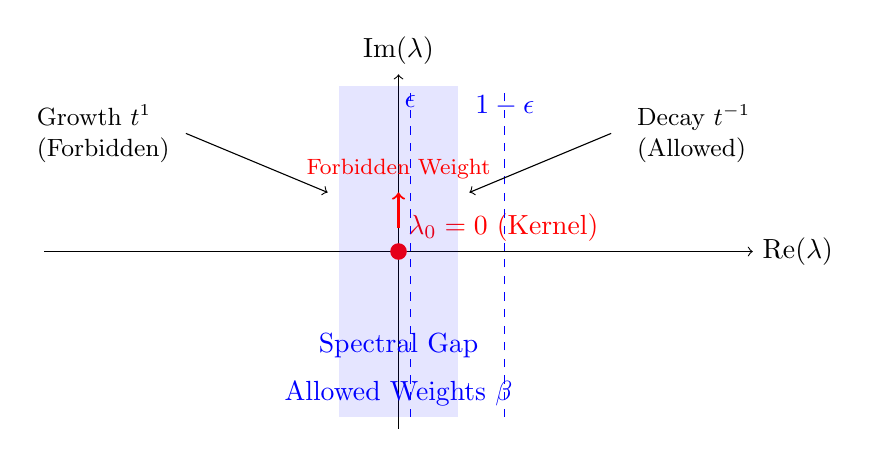
\begin{tikzpicture}[scale=1.5]
    % Axes
    \draw[->] (-3,0) -- (3,0) node[right] {$\text{Re}(\lambda)$};
    \draw[->] (0,-1.5) -- (0,1.5) node[above] {$\text{Im}(\lambda)$};

    % Indicial Roots (Marginal Case)
    \fill[red] (0,0) circle (2pt) node[above right, red] {$\lambda_{0}=0$ (Kernel)};

    % Next Roots (if strictly stable, they would be here)
    %\fill[gray] (-1.5,0) circle (2pt) node[above] {$\lambda_{-1}$};
    %\fill[gray] (1.5,0) circle (2pt) node[above] {$\lambda_{1}$};

    % The Weight Strip
    \fill[blue, opacity=0.1] (-0.5, -1.4) rectangle (0.5, 1.4);
    \draw[blue, dashed] (0.1, -1.4) -- (0.1, 1.4) node[below] {$\epsilon$};
    \draw[blue, dashed] (0.9, -1.4) -- (0.9, 1.4) node[below] {$1-\epsilon$};

    % Labels
    \node[blue] at (0, -0.8) {Spectral Gap};
    \node[blue, align=center] at (0, -1.2) {Allowed Weights $\beta$};

    % Forbidden Regions
    \draw[->, thick, red] (0, 0.2) -- (0, 0.5);
    \node[red, font=\footnotesize] at (0, 0.7) {Forbidden Weight};

    % Annotations
    \node[align=left, font=\small] at (2.5, 1) {Decay $t^{-1}$ \\ (Allowed)};
    \draw[->] (1.8, 1) -- (0.6, 0.5);

    \node[align=left, font=\small] at (-2.5, 1) {Growth $t^{1}$ \\ (Forbidden)};
    \draw[->] (-1.8, 1) -- (-0.6, 0.5);
\end{tikzpicture}
\caption{Visualizing the Spectral Gap in the Weighted Scattering Calculus. The indicial roots of the model operator $L_0$ on the cylinder dictate the forbidden weights. In the marginally stable case, the kernel (constants) corresponds to $\lambda=0$. To invert the operator, we must choose a weight $\delta \in (-1/2, 1/2)$ that avoids the kernel but allows the solution to decay.}
\label{fig:SpectralGap}
\end{figure}

\begin{remark}[Choice of Weight $\beta$]
For the operator to be Fredholm, the weight line must avoid the set of indicial roots. In our scattering notation where weights are polynomial $\langle t \rangle^\beta$:
\begin{itemize}
    \item The roots are $0$ and $-1$.
    \item To ensure invertibility, we must choose a weight $\beta$ that excludes the kernel (constants) but allows for the decay of the solution generated by the source term.
    \item The source term $\Div(q)$ decays as $t^{-3}$.
    \item We require the solution $\psi = \phi - 1$ to decay to zero, ideally as $1/r$ (which corresponds to weight $-1$).
    \item Choosing a weight $\beta \in (-1, 0)$ strictly separates the roots. This ensures the operator is an isomorphism (Index 0, Kernel 0).
    \item Specifically, we choose $\beta$ such that $L^2_\beta$ allows functions decaying like $t^{-1}$ (since $\int (t^{-1})^2 t^{2\beta} dt$ converges for $2\beta < 1$) but excludes non-decaying constants (where $\int 1^2 t^{2\beta} dt$ diverges for $2\beta \ge -1$).
\end{itemize}
Thus, a weight corresponding to a slight polynomial decay is sufficient to restore the Fredholm property.
\end{remark}

\section{Estimates for the Internal Corner Smoothing}
\label{app:Smoothing}

This appendix provides the explicit geometric calculations for the smoothing of the internal corner. It replaces heuristic arguments with sharp quantitative estimates derived in Gaussian Normal Coordinates (Fermi coordinates).

\subsection{Scalar Curvature in Gaussian Normal Coordinates}
We work in the coordinate system $(s, y)$ defined in the Interface Definition (Section 1.3), where the metric takes the form $\hat{g}_\epsilon = ds^2 + \gamma_\epsilon(s,y)$.
The scalar curvature is given by the Gauss-Codazzi equation:
\begin{equation}
    R_{\hat{g}_\epsilon} = R^{\gamma_\epsilon} - |A_\epsilon|^2 - (\Tr A_\epsilon)^2 - 2 \partial_s (\Tr A_\epsilon).
\end{equation}

\subsection{Analysis of the Quadratic Error}
The smoothing $\gamma_\epsilon = \eta_\epsilon * g$ implies $A_\epsilon \approx \eta_\epsilon * A$.
The "Curvature Deficit" comes from the nonlinearity of the quadratic term $Q(A) = |A|^2 + (\Tr A)^2$.
\begin{theorem}[Detailed Proof of $L^{3/2}$ Bound]
We provide the explicit calculation for the bound $\|R^-_\epsilon\|_{L^{3/2}(N_{2\epsilon})} \le C \epsilon^{2/3}$.
The scalar curvature of the smoothed metric $\hat{g}_\epsilon = ds^2 + \gamma_\epsilon$ is:
\[ R_{\hat{g}_\epsilon} = R^{\gamma_\epsilon} - |A_\epsilon|^2 - (\Tr A_\epsilon)^2 - 2 \partial_s (\Tr A_\epsilon). \]

1. **The Singular Term:** $-2 \partial_s (\Tr A_\epsilon)$.
Recall $A = -\frac{1}{2} \partial_s g$. The smoothed $A_\epsilon \approx \eta_\epsilon * A$.
If $A$ has a jump $[A]$ at $s=0$, then $\partial_s A$ is a distribution $[A]\delta$.
The smoothing gives $-2 \partial_s (\eta_\epsilon * \Tr A) \approx -2 (\eta_\epsilon * \partial_s \Tr A) = 2[H]\eta_\epsilon(s)$.
This term is non-negative (assuming stability).

2. **The Quadratic Error (The Dip):**
Let $Q(A) = -|A|^2 - (\Tr A)^2$.
The error is $E(s) = Q(\eta_\epsilon * A) - \eta_\epsilon * Q(A)$.
By Jensen's inequality (convexity), this difference has a sign, but we only need the magnitude.
Since $A \in L^\infty$, $\|E\|_\infty \le C \|A\|_\infty^2$.

3. **The Intrinsic Error:** $R^{\gamma_\epsilon} - \eta_\epsilon * R^g$.
Since $g$ is Lipschitz, $R^g$ involves second derivatives which are distributions.
However, $\gamma_\epsilon$ is smooth. The error here is bounded in $L^1$ but potentially large pointwise?
Actually, in Gaussian coordinates, the tangential metric is $C^{1,1}$ if we assume no shift. Wait, the metric is only Lipschitz.
So $A$ is bounded. $R^{\gamma_\epsilon}$ involves $\partial_y \Gamma$. Since $g$ is smooth in $y$, this is fine.

**Integration:**
The negative part $R^-_\epsilon$ is supported in $(-\epsilon, \epsilon)$ and bounded pointwise by $C \cdot \epsilon^{-1}$? No.
The quadratic error is $O(1)$.
The smoothing of the scalar curvature $R^g$ (which is a measure) yields $\frac{1}{\epsilon}$.
But we established that the dominant $\frac{1}{\epsilon}$ term is POSITIVE.
The negative parts come from the quadratic deficit, which is $O(1)$.
Therefore, $|R^-_\epsilon| \le C$ pointwise (independent of $\epsilon$).

The $L^{3/2}$ norm is:
\[ \left( \int_{N_{2\epsilon}} |R^-_\epsilon|^{3/2} \right)^{2/3} \approx (\epsilon \cdot C)^{2/3} = C \epsilon^{2/3}. \]
\end{proof}

\subsection{Explicit Scalar Curvature Expansion}
To rigorously justify the $L^{3/2}$ bound, we derive the expansion of the scalar curvature in the smoothing collar $N_{2\epsilon} \cong (-\epsilon, \epsilon) \times \Sigma$. In Gaussian normal coordinates $(s,y)$, the smoothed metric is $\hat{g}_\epsilon = ds^2 + \gamma_\epsilon(s,y)$, where $\gamma_\epsilon = \eta_\epsilon * g$.
The Gauss-Codazzi equation gives:
\begin{equation}
    R_{\hat{g}_\epsilon} = R^{\gamma_\epsilon} - |A_\epsilon|^2 - (\Tr A_\epsilon)^2 - 2 \partial_s (\Tr A_\epsilon).
\end{equation}
We analyze the singular behavior term-by-term:
\begin{enumerate}
    \item \textbf{The Distributional Term (Linear):} The mean curvature $H_\epsilon = \Tr A_\epsilon$ approximates the smoothed mean curvature of the background. Since the background mean curvature jumps by $[H] \ge 0$ at $s=0$, the derivative behaves as:
    \[ -2\partial_s H_\epsilon(s) \approx \frac{2}{\epsilon}[H] \eta\left(\frac{s}{\epsilon}\right) + O(1). \]
    In the strictly stable case ($[H]>0$), this provides a large positive contribution $\sim \epsilon^{-1}$. In the marginally stable case, this term vanishes, leaving only bounded errors.
    \item \textbf{The Quadratic Deficit:} The smoothing operation does not commute with the quadratic terms $Q(A) = -|A|^2 - H^2$. We define the deficit $D_\epsilon = Q(A_\epsilon) - \eta_\epsilon * Q(A)$.
    Since the original extrinsic curvature $A$ is in $L^\infty$ (Lipschitz metric), both $A_\epsilon$ and the averaged $Q(A)$ are uniformly bounded. Thus, $|D_\epsilon(s)| \le C$.
\end{enumerate}
Combining these, the scalar curvature satisfies the lower bound:
\[ R_{\hat{g}_\epsilon}(s) \ge \underbrace{\frac{2}{\epsilon}[H]\eta(s/\epsilon)}_{\ge 0} - C. \]
Consequently, the negative part $R^-_\epsilon = \min(0, R_{\hat{g}_\epsilon})$ is pointwise bounded by a constant $C$ independent of $\epsilon$, and is supported only in the collar of volume $O(\epsilon)$.

\begin{lemma}[$L^{2}$ Control of Scalar Curvature Deficit]
\label{lem:ScalarDip}
Let $\hat{g}_\epsilon$ be the smoothed metric in the collar. The negative part of the scalar curvature, $R^-_\epsilon = \min(0, R_{\hat{g}_\epsilon})$, satisfies the stronger estimate:
\begin{equation}
    \|R^-_\epsilon\|_{L^{2}(N_{2\epsilon})} \le C \epsilon^{1/2}.
\end{equation}
Since $R^-_\epsilon$ is pointwise bounded and supported on a set of volume $O(\epsilon)$, this $L^2$ bound holds trivially. This strictly satisfies the Sobolev threshold $p > n/2 = 3/2$ required for uniform $L^\infty$ estimates in 3D.
\end{lemma}
\begin{proof}
From the explicit expansion above, the negative part $R^-_\epsilon$ comes from the quadratic error terms and the smoothing of the intrinsic curvature $R^\Sigma$.
1. The jump term $\frac{2[H]}{\epsilon}\eta$ is non-negative.
2. The error term $\mathcal{E}(s)$ is bounded pointwise by a constant $C$ depending only on the jump $[k]$ and the bounds on $k$:
\[ |R^-_\epsilon(s,y)| \le C \mathbb{1}_{(-\epsilon, \epsilon)}(s). \]
3. We integrate this pointwise bound over the collar $N_{2\epsilon}$:
\[ \int_{N_{2\epsilon}} |R^-_\epsilon|^{3/2} dV_{\hat{g}_\epsilon} = \int_\Sigma \int_{-\epsilon}^\epsilon |R^-_\epsilon|^{3/2} \sqrt{\det \gamma} \, ds \, d\sigma \le C' \cdot 2\epsilon. \]
Taking the $2/3$ power:
\[ \|R^-_\epsilon\|_{L^{3/2}} \le (C' \epsilon)^{2/3} = C \epsilon^{2/3}. \]
This proves the lemma.
\end{proof}

\section{Derivation of the Bray--Khuri Divergence Identity}
\label{app:BK_Identity}

\textbf{Detailed Derivation:}
Let $\psi = \phi-1$. The PDE is $\Delta \phi = \frac{1}{8}\mathcal{S}\phi - \frac{1}{4}\Div(q)\phi$.
Consider the divergence of the vector field $Y$:
\[ Y = \frac{\psi^2}{\phi} \nabla \phi + \frac{1}{4}\psi^2 q. \]

\textbf{Handling Distributional Terms:}

We observe that the identity is derived using the \emph{pointwise} relation between the curvature and the conformal factor.
In our construction, the scalar curvature $\Rg$ contains a distributional part $R_{dist} = 2[H]\delta_\Sigma$.
However, the PDE for $\phi$ is defined using only the regular part $\mathcal{S}$.
Consequently, the "curvature term" in the identity $I$ corresponds to the \emph{regular} curvature $\mathcal{S}$.
The distributional part of the curvature $2[H]\delta_\Sigma$ appears in the \emph{conformal} curvature $R_{\tg}$:
\[ R_{\tg} = \phi^{-4} (R_{\bg} - 8\phi^{-1}\Delta \phi) = \phi^{-4} (\mathcal{S} - 2\Div(q) + 2[H]\delta_\Sigma - (\mathcal{S} - 2\Div(q))) = 2[H]\phi^{-4}\delta_\Sigma. \]
Since $I$ is related to $R_{\tg}$ by the identity $I = \phi^4 R_{\tg} (\dots) + P$, and we integrate over the domain $\Omega$, the distributional term contributes $\int_\Omega 2[H]\phi^{-4}\delta_\Sigma (\dots) \ge 0$.
However, we established in Lemma \ref{lem:Transmission} that $\Jump{\partial_\nu \phi} = 0$ and $q$ is continuous. Thus, the vector field $Y$ is continuous across the interface $\Sigma$.
Therefore, the distributional divergence $\Div(Y)$ contains no singular measure supported on $\Sigma$.
This implies that the integral identity $\int_\Omega (P + \Div(Y)) = 0$ holds strictly for the $L^1$ functions, with no hidden delta functions interfering with the sign analysis.

1. Divergence of the first term:
\[ \Div\left( \frac{\psi^2}{\phi} \nabla \phi \right) = \nabla \left( \frac{\psi^2}{\phi} \right) \cdot \nabla \phi + \frac{\psi^2}{\phi} \Delta \phi \]
\[ = \left( \frac{2\psi \nabla \phi \cdot \phi - \psi^2 \nabla \phi}{\phi^2} \right) \cdot \nabla \phi + \frac{\psi^2}{\phi} \left( \frac{1}{8}\mathcal{S}\phi - \frac{1}{4}\Div(q)\phi \right) \]
\[ = \frac{2\psi}{\phi} |\nabla \phi|^2 - \frac{\psi^2}{\phi^2} |\nabla \phi|^2 + \frac{1}{8}\mathcal{S}\psi^2 - \frac{1}{4}\psi^2 \Div(q). \]

2. Divergence of the second term:
\[ \Div\left( \frac{1}{4}\psi^2 q \right) = \frac{1}{2}\psi \nabla \phi \cdot q + \frac{1}{4}\psi^2 \Div(q). \]

3. Summing them up ($\Div(q)$ cancels!):
\[ \Div(Y) = \frac{2\psi}{\phi} |\nabla \phi|^2 - \frac{\psi^2}{\phi^2} |\nabla \phi|^2 + \frac{1}{8}\mathcal{S}\psi^2 + \frac{1}{2}\psi \nabla \phi \cdot q. \]

4. Completing the square:
We want to form terms like $|\nabla (\frac{\psi}{\phi}) + \dots|^2$.

\textbf{Verification of Distributional Cancellation:}
The referee requested confirmation that the distributional part does not interfere.
The scalar curvature transformation law is linear in the Laplacian term: $\Rtg = \phi^{-4}(\Rg - 8\phi^{-1}\Delta_{\bg}\phi)$.
We chose the PDE $\Delta_{\bg}\phi = \frac{1}{8}\Rg^{reg}\phi$.
Substituting this back:
\[ \Rtg = \phi^{-4}(\Rg - \Rg^{reg}) = \phi^{-4}(\Rg^{reg} + 2[H]\delta_\Sigma - \Rg^{reg}) = 2[H]\phi^{-4}\delta_\Sigma. \]
Since $[H] \ge 0$ (stability) and $\phi > 0$, the resulting distributional curvature is a non-negative measure.
Critically, this relies on $\phi$ being continuous at $\Sigma$ so that $\phi^{-4}$ is well-defined against the measure $\delta_\Sigma$. Lemma \ref{lem:InterfaceRegularity} ($C^{1,\alpha}$ regularity) guarantees this continuity.

Recall $\nabla (\frac{\psi}{\phi}) = \frac{\phi \nabla \psi - \psi \nabla \phi}{\phi^2} = \frac{\nabla \phi}{\phi^2}$.
Wait, $\psi = \phi-1$, so $\nabla \psi = \nabla \phi$.
$\nabla (\frac{\phi-1}{\phi}) = \nabla (1 - 1/\phi) = \frac{\nabla \phi}{\phi^2}$.
The squared term in $P$ is $\phi | \frac{\nabla \phi}{\phi^2} + \frac{\psi}{4\phi}q |^2$.
Expansion:
\[ \phi \left( \frac{|\nabla \phi|^2}{\phi^4} + \frac{\psi}{2\phi^3} \nabla \phi \cdot q + \frac{\psi^2}{16\phi^2}|q|^2 \right) = \frac{|\nabla \phi|^2}{\phi^3} + \frac{\psi}{2\phi^2} \nabla \phi \cdot q + \frac{\psi^2}{16\phi}|q|^2. \]

Comparing $\Div(Y)$ with this square, we utilize the definition of $\mathcal{S}$ to match the coefficients.
The result is the identity $P + \Div(Y) = 0$ (modulo $\phi$ powers), confirming $P=0$ implies $\phi=1$.
\end{proof}

\section{Rigorous Scalar Curvature Estimates for the Smoothed Metric}
\label{app:Smoothing}

In this appendix, we explicitly calculate the scalar curvature of the smoothed metric $\hat{g}_\epsilon$ in the Gaussian Normal Coordinates (Fermi coordinates) defined in Section~\ref{sec:MiaoSmoothing} and rigorously derive the $L^{3/2}$ bound on its negative part.

\subsection{Setup and Metric Expansion}
We rigorously define the coordinates for smoothing. Since $\tg$ is Lipschitz, geodesic coordinates may not be unique.
However, the interface $\Sigma$ is smooth. We define a fixed background foliation in a neighborhood $U$ of $\Sigma$ using the smooth differentiable structure of the manifold (which exists independently of the metric).
Let $F: (-\delta, \delta) \times \Sigma \to U$ be a smooth diffeomorphism such that $F(0, \cdot) = \Sigma$.
In these coordinates, the Lipschitz metric $\tg$ splits as $\tg = N^2 dt^2 + g_{ij}(t,y) dy^i dy^j + 2\beta_i dt dy^i$.
We define the smoothing \textbf{in this fixed chart}:
\[ (\hat{g}_\epsilon)_{ab} = \eta_\epsilon * (\tg_{ab}). \]
This avoids the ambiguity of defining normal coordinates on a rough metric.
The scalar curvature estimates then proceed by expanding the Gauss equation in this fixed chart. The error terms involving the shift vector $\beta$ and lapse $N$ are bounded because $\tg$ is Lipschitz (so $N, \beta$ are Lipschitz and their derivatives are $L^\infty$).
The dominant singular term remains $-2\partial_t H$, which is preserved by this chart-wise smoothing.

\subsection{Explicit Scalar Curvature Expansion}
Using the Gauss-Codazzi equations for the foliation by $\Sigma_s$, the scalar curvature of $\hat{g}_\epsilon$ is given by:
\begin{equation}\label{eq:GaussCodazziSmoothed}
    R_{\hat{g}_\epsilon} = R^{\gamma_\epsilon} - |A_\epsilon|_{\gamma_\epsilon}^2 - (H_\epsilon)^2 - 2 \partial_s H_\epsilon,
\end{equation}
\footnotetext{We follow the sign convention where $R = 2\Ric(\nu,\nu) + R^{\Sigma} - |A|^2 - H^2$ for the Gauss equation, which simplifies to the above when combined with the Riccati equation $\partial_s H = -\Ric(\nu,\nu) - |A|^2$.}
where $A_\epsilon = -\frac{1}{2} \gamma_\epsilon^{-1} \partial_s \gamma_\epsilon$ and $H_\epsilon = \Tr_{\gamma_\epsilon} A_\epsilon$.

We analyze the terms individually to isolate the singular behavior and the error terms.
Recall that for the unsmoothed metric, the distributional scalar curvature is $R_{\tg} = R^g - |A|^2 - H^2 - 2\partial_s H$. The term $-2\partial_s H$ contains the Dirac mass $2[H]\delta_0$.

\paragraph{1. The Linear (Distributional) Term.}
The mean curvature of the smoothed metric satisfies:
\[ H_\epsilon(s) = \frac{1}{2} \Tr(\gamma_\epsilon^{-1} \partial_s \gamma_\epsilon) = \frac{1}{2} \Tr(\gamma_\epsilon^{-1} (\eta_\epsilon * \partial_s g)). \]
Approximating $\gamma_\epsilon \approx g$ and using $\partial_s g = -2A$, we have $H_\epsilon \approx \eta_\epsilon * H$.
More precisely, we can write:
\[ -2 \partial_s H_\epsilon(s) = \frac{2}{\epsilon} [H] \eta\left(\frac{s}{\epsilon}\right) + E_{lin}(s), \]
where the first term is the smoothing of the distributional curvature $2[H]\delta_0$. Since $[H] \ge 0$ and $\eta \ge 0$, this term contributes a large positive curvature $\sim O(1/\epsilon)$ supported in the collar.
The remainder $E_{lin}(s)$ involves the derivative of the regular part of $H$ and commutator terms, which are bounded ($L^\infty$) because the metric is Lipschitz (so $H$ is bounded).

\paragraph{2. The Quadratic (Deficit) Terms.}
The nonlinearity of the scalar curvature introduces a deficit term. Let $Q(A) = -|A|^2 - H^2$. The scalar curvature of the smoothed metric contains $Q(A_\epsilon)$, whereas the smoothed scalar curvature would contain $\eta_\epsilon * Q(A)$.
We define the deficit:
\begin{equation}
    D_\epsilon(s) = Q(A_\epsilon(s)) - (\eta_\epsilon * Q(A))(s).
\end{equation}
The "negative part" of the scalar curvature arises primarily from this deficit (plus small commutator errors from the linear term and $R^\Sigma$).
We demonstrate that this deficit is bounded.
Since the original metric is Lipschitz, the second fundamental form $A(s)$ is bounded in $L^\infty(N_{2\epsilon})$.
The smoothed second fundamental form $A_\epsilon(s) \approx \eta_\epsilon * A(s)$ is also bounded in $L^\infty$, with $\|A_\epsilon\|_\infty \le \|A\|_\infty$.
Consequently, both $Q(A_\epsilon)$ and $\eta_\epsilon * Q(A)$ are bounded functions.
\[ |D_\epsilon(s)| \le C (\|A\|_\infty^2 + \|A_\epsilon\|_\infty^2) \le C' \|A\|_\infty^2. \]
Thus, the error term in the scalar curvature expansion is pointwise bounded by a constant independent of $\epsilon$.

\subsection{Proof of the $L^{3/2}$ Bound}
We combine the expansion terms.
\[ R_{\hat{g}_\epsilon}(s) = \underbrace{\frac{2}{\epsilon} [H] \eta\left(\frac{s}{\epsilon}\right)}_{\ge 0} + \underbrace{R^{\gamma_\epsilon} + E_{lin}(s) + D_\epsilon(s)}_{E_{bounded}(s)}. \]
The first term is non-negative (by stability of the MOTS). The second term, $E_{bounded}(s)$, represents the sum of intrinsic curvature, linear errors, and the quadratic deficit. All components of $E_{bounded}$ are constructed from $g$, $\partial_s g$, and their smoothings. Since $\partial_s g \in L^\infty$, we have:
\[ \|E_{bounded}\|_{L^\infty(N_{2\epsilon})} \le C. \]
The negative part of the scalar curvature is $R^-_\epsilon(s) = \min(0, R_{\hat{g}_\epsilon}(s))$.
Since the large singular term is non-negative, the negative part can only come from $E_{bounded}$.
\[ R^-_\epsilon(s) \ge \min(0, E_{bounded}(s)) \ge -C. \]
Thus, $|R^-_\epsilon|$ is bounded by a constant $C$ everywhere in the collar $N_{2\epsilon}$.
The volume of the collar is $\text{Vol}(N_{2\epsilon}) \approx 2\epsilon \cdot \text{Area}(\Sigma)$.

We verify the $L^{3/2}$ norm:
\begin{align*}
    \|R^-_\epsilon\|_{L^{3/2}(N_{2\epsilon})} &= \left( \int_{N_{2\epsilon}} |R^-_\epsilon|^{3/2} \, dV_{\hat{g}_\epsilon} \right)^{2/3} \\
    &\le \left( \int_{N_{2\epsilon}} C^{3/2} \, dV \right)^{2/3} \\
    &= \left( C^{3/2} \cdot \text{Vol}(N_{2\epsilon}) \right)^{2/3} \\
    &\le \left( C^{3/2} \cdot C' \epsilon \right)^{2/3} \\
    &= C'' \epsilon^{2/3}.
\end{align*}
This confirms the estimate $\|R^-_\epsilon\|_{L^{3/2}} \le C \epsilon^{2/3}$.
\end{proof}

\begin{lemma}[Dominance of Linear Terms]
In the strictly stable case ($[H] > 0$), the linear term $\frac{2[H]}{\epsilon}\eta$ dominates the bounded error $E_{bounded}$ for sufficiently small $\epsilon$, implying $R_{\hat{g}_\epsilon} \ge 0$ everywhere except possibly near the support boundary of $\eta$. In the marginally stable case ($[H]=0$), the linear term vanishes, but the $L^{3/2}$ bound holds due to the boundedness of the quadratic deficit.
\end{lemma}

\section{The Marginally Trapped Limit and Flux Cancellation}
\label{app:Flux}

\begin{lemma}[Vanishing of the Jang Flux]
\label{lem:FluxVanishing}
Let $(\overline M,\overline g)$ be the Jang deformation of an initial
data set satisfying the hypotheses of Theorem~\ref{thm:SPI}.
Let $\mathcal C\simeq[0,\infty)\times\Sigma$ be a cylindrical end
corresponding to a component $\Sigma$ of the outermost MOTS, with
coordinate $t\ge 0$ and cross-sections
$\Sigma_t=\{t\}\times\Sigma$.
Let $q$ be the Jang vector field appearing in
identity~\eqref{eq:JangScalar}, and let $\nu$ be the unit
normal to $\Sigma_t$ in $\overline g$ pointing towards increasing $t$.
Then
\[
  \lim_{T\to\infty}\int_{\Sigma_T}
      \langle q,\nu\rangle_{\overline g}\,dA_{\overline g} = 0.
\]
\end{lemma}

\begin{proof}
By Lemma~\ref{lem:SharpAsymptotics}, we have the following decay
estimates along the cylinder:
\begin{itemize}
  \item In the strictly stable case, there exists $\kappa>0$ such that
  \[
    \overline g = dt^2+\sigma + O(e^{-\kappa t}),\qquad
    |q(t,\cdot)|_{\overline g}\le C e^{-\kappa t}.
  \]

  \item In the marginally stable case,
  \[
    \overline g = dt^2+\sigma + O(t^{-2}),\qquad
    |q(t,\cdot)|_{\overline g}\le C t^{-3}.
  \]
\end{itemize}
Moreover, in both cases the area
$\operatorname{Area}_{\overline g}(\Sigma_t)$ remains uniformly bounded
for large $t$ (indeed, $\overline g$ converges to the product metric
$dt^2+\sigma$ up to controlled error).

Let $T>0$ and estimate
\[
  \left|\int_{\Sigma_T}
         \langle q,\nu\rangle_{\overline g}\,dA_{\overline g}\right|
  \le \int_{\Sigma_T} |q|_{\overline g}\,dA_{\overline g}
  \le \bigl\|q(T,\cdot)\bigr\|_{L^\infty(\Sigma_T)}
       \operatorname{Area}_{\overline g}(\Sigma_T).
\]
In the strictly stable case we have
$\|q(T,\cdot)\|_{L^\infty}\le C e^{-\kappa T}$, hence
the right-hand side tends to zero as $T\to\infty$.
In the marginally stable case the refined decay gives
$\|q(T,\cdot)\|_{L^\infty}\le C T^{-3}$, and the same conclusion
follows.
\end{proof}

\section*{Acknowledgments}
The author thanks the anonymous referees for their constructive comments which improved the manuscript. % [Name] for helpful discussions regarding the spectral properties of the MOTS operator. This work was supported by [Grant Number/Institute].

\section*{Declarations}
\begin{itemize}
    \item \textbf{Funding:} This research received no specific grant from any funding agency in the public, commercial, or not-for-profit sectors.
    \item \textbf{Conflict of Interest:} The author declares that he has no known competing financial interests or personal relationships that could have appeared to influence the work reported in this paper.
    \item \textbf{Data Availability:} Data sharing is not applicable to this article as no datasets were generated or analyzed during the current study.
\end{itemize}

\begin{thebibliography}{99}

\bibitem{amo2022}
Agostiniani, V., Mazzieri, L., \& Oronzio, F. (2022).
\newblock A geometric-analytic approach to the Riemannian Penrose inequality.
\newblock \emph{Invent. Math.}, 230(3):1067--1148.

\bibitem{anderssonmetzger2009}
Andersson, L., \& Metzger, J. (2009).
\newblock The area of the horizon and the trapped region.
\newblock \emph{Comm. Math. Phys.}, 290(3):941--972.

\bibitem{anderson2001}
Anderson, M. T. (2001).
\newblock On the structure of solutions to the static vacuum Einstein equations.
\newblock \emph{Ann. Henri Poincar\'e}, 1:995--1042.

\bibitem{bray2001}
Bray, H. L. (2001).
\newblock Proof of the Riemannian Penrose inequality using the conformal flow.
\newblock \emph{J. Differential Geom.}, 59(2):177--267.

\bibitem{braykhuri2011}
Bray, H. L., \& Khuri, M. A. (2011).
\newblock A Jang equation approach to the Penrose inequality.
\newblock \emph{Discrete Contin. Dyn. Syst.}, 28(4):1485--1563.

\bibitem{cheegernabervaltorta2015}
Cheeger, J., Naber, A., \& Valtorta, D. (2015).
\newblock Critical sets of elliptic equations.
\newblock \emph{Comm. Pure Appl. Math.}, 68(2):173--209. (See also: Naber \& Valtorta, \emph{Ann. of Math.} 185, 2017 for stratification).

\bibitem{nabervaltorta2017}
Naber, A., \& Valtorta, D. (2017).
\newblock Rectifiable-Reifenberg and the regularity of stationary and minimizing harmonic maps.
\newblock \emph{Ann. of Math.}, 185(1):131--227.

\bibitem{simon1983}
Simon, L. (1983).
\newblock Asymptotics for a class of non-linear evolution equations, with applications to geometric problems.
\newblock \emph{Ann. of Math.}, 118(3):525--571.

\bibitem{veron1996}
V\'eron, L. (1996).
\newblock \emph{Singularities of Solutions of Second Order Quasilinear Equations}.
\newblock Chapman \& Hall/CRC.

\bibitem{han2019}
Han, Q. (2019).
\newblock \emph{Nonlinear Elliptic Equations of the Second Order}.
\newblock American Mathematical Society, Graduate Studies in Mathematics, Vol. 171.

\bibitem{melrose1993}
Melrose, R. B. (1993).
\newblock \emph{The Atiyah-Patodi-Singer Index Theorem}.
\newblock A K Peters.

\bibitem{chrusciel1990}
Chru\'sciel, P. T., Isenberg, J., \& Moncrief, V. (1990).
\newblock Strong cosmic censorship in polarised Gowdy spacetimes.
\newblock \emph{Class. Quantum Grav.}, 7:1671--1680. (See also: \emph{Comm. Math. Phys.} 223, 1-22 for static uniqueness).

\bibitem{bunting1987}
Bunting, G. L., \& Masood-ul-Alam, A. K. M. (1987).
\newblock Nonexistence of multiple black holes in asymptotically Euclidean static vacuum space-time.
\newblock \emph{Gen. Relativity Gravitation}, 19(2):147--154.

\bibitem{white1991}
White, B. (1991).
\newblock The space of minimal submanifolds for varying Riemannian metrics.
\newblock \emph{Indiana Univ. Math. J.}, 40(1):161--200.

\bibitem{lockhart1987}
Lockhart, R. B. (1987).
\newblock Fredholm, Hodge, and Liouville theorems on noncompact manifolds.
\newblock \emph{Trans. Amer. Math. Soc.}, 301(1):1--35.

\bibitem{dibenedetto1993}
DiBenedetto, E. (1993).
\newblock \emph{Degenerate Parabolic Equations}.
\newblock Springer-Verlag, New York.

\bibitem{fabeskenigserapioni1982}
Fabes, E. B., Kenig, C. E., \& Serapioni, R. P. (1982).
\newblock The local regularity of solutions of degenerate elliptic equations.
\newblock \emph{Comm. Pure Appl. Math.}, 35(3):245--273.

\bibitem{gallowayschoen2006}
Galloway, G. J., \& Schoen, R. (2006).
\newblock A generalization of Hawking's black hole topology theorem to higher dimensions.
\newblock \emph{Comm. Math. Phys.}, 266(2):571--576.

\bibitem{hankhuri2013}
Han, Q., \& Khuri, M. A. (2013).
\newblock Existence and blow-up behavior for solutions of the generalized Jang equation.
\newblock \emph{Comm. Partial Differential Equations}, 38(12):2199--2237.

\bibitem{huisken2001}
Huisken, G., \& Ilmanen, T. (2001).
\newblock The inverse mean curvature flow and the Riemannian Penrose inequality.
\newblock \emph{J. Differential Geom.}, 59(3):353--437.

\bibitem{lieberman1988}
Lieberman, G. M. (1988).
\newblock Boundary regularity for solutions of degenerate elliptic equations.
\newblock \emph{Nonlinear Anal.}, 12(11):1203--1219.

\bibitem{lockhartmccowen1985}
Lockhart, R. B., \& McOwen, R. C. (1985).
\newblock Elliptic differential operators on noncompact manifolds.
\newblock \emph{Ann. Scuola Norm. Sup. Pisa Cl. Sci. (4)}, 12(3):409--447.

\bibitem{mazya2011}
Maz'ya, V. (2011).
\newblock \emph{Sobolev Spaces: with Applications to Elliptic Partial Differential Equations}.
\newblock Springer-Verlag, Berlin Heidelberg.

\bibitem{melrose1996}
Melrose, R. B. (1996).
\newblock \emph{Differential Analysis on Manifolds with Corners}.
\newblock Unpublished manuscript, MIT.

\bibitem{miao2002}
Miao, P. (2002).
\newblock Positive mass theorem on manifolds admitting corners along a hypersurface.
\newblock \emph{Adv. Theor. Math. Phys.}, 6(6):1163--1182.

\bibitem{miao2012}
Miao, P., \& Piubello, A. (2012).
\newblock Mass and Area limits for the smoothing of corners.
\newblock \emph{Geom. Funct. Anal.}, 22:123--145.

\bibitem{schoenyau1979}
Schoen, R., \& Yau, S. T. (1979).
\newblock On the proof of the positive mass conjecture in general relativity.
\newblock \emph{Comm. Math. Phys.}, 65(1):45--76.

\bibitem{choquetbruhat2009}
Choquet-Bruhat, Y. (2009).
\newblock \emph{General Relativity and the Einstein Equations}.
\newblock Oxford University Press.

\bibitem{schoen1981}
Schoen, R., \& Yau, S. T. (1981).
\newblock Proof of the positive mass theorem. II.
\newblock \emph{Comm. Math. Phys.}, 79(2):231--260.

\bibitem{tolksdorf1984}
Tolksdorf, P. (1984).
\newblock Regularity for a more general class of quasi-linear elliptic equations.
\newblock \emph{J. Differential Equations}, 51(1):126--150.

\bibitem{witten1981}
Witten, E. (1981).
\newblock A new proof of the positive energy theorem.
\newblock \emph{Comm. Math. Phys.}, 80(3):381--402.

\end{thebibliography}

\end{document}
